\pdfinfoomitdate=1
\pdftrailerid{}
\pdfsuppressptexinfo=15
\documentclass[11pt]{article}
\usepackage[T1]{fontenc}
\usepackage[utf8]{inputenc}
\usepackage{lmodern}
\usepackage[margin=1in]{geometry}
\usepackage{amsmath,amssymb,amsthm,mathtools}
\usepackage{booktabs,longtable,array}
\usepackage{listings}
\usepackage{microtype}
\usepackage{graphicx}
\usepackage{tikz}
\usetikzlibrary{arrows.meta,calc,positioning,decorations.pathreplacing}
\usepackage{needspace,flafter,placeins}
\usepackage[numbers,sort&compress]{natbib}
\usepackage{xurl}
\usepackage[colorlinks=true,linkcolor=blue!45!black,citecolor=blue!45!black,urlcolor=blue!45!black]{hyperref}
\def\UrlBreaks{\do\/\do\-}
\hypersetup{pdftitle={Universal optimality of the triangular lattice},pdfauthor={OpenAI}}
\newcommand{\R}{\mathbb R}
\newcommand{\C}{\mathbb C}
\newcommand{\Z}{\mathbb Z}
\newcommand{\N}{\mathbb N}
\newcommand{\dd}{\mathop{}\!\mathrm d}
\newcommand{\norm}[1]{\left\lVert#1\right\rVert}
\newcommand{\abs}[1]{\left\lvert#1\right\rvert}
\DeclareMathOperator{\Rea}{Re}
\DeclareMathOperator{\Ima}{Im}
\DeclareMathOperator{\supp}{supp}
\DeclareMathOperator{\vol}{vol}
\newtheorem{theorem}{Theorem}[section]
\newtheorem{lemma}[theorem]{Lemma}
\newtheorem{proposition}[theorem]{Proposition}
\newtheorem{corollary}[theorem]{Corollary}
\theoremstyle{definition}
\newtheorem{definition}[theorem]{Definition}
\theoremstyle{remark}
\newtheorem{remark}[theorem]{Remark}
\numberwithin{equation}{section}

\setlength{\emergencystretch}{1.5em}
\lstset{basicstyle=\ttfamily\footnotesize,columns=fullflexible,keepspaces=true,
  showstringspaces=false,breaklines=true,frame=single,framerule=.2pt}
\title{Universal optimality of the triangular lattice}
\author{OpenAI}
\date{September 23, 2026}
\begin{document}
\maketitle
\begin{abstract}
We prove universal energy minimality for the triangular lattice in the plane.
Among locally finite configurations of centered density one, it minimizes the
lower limit of centered-ball energy averages for every nonnegative completely
monotone function of squared distance, including when the energy is infinite.
We also prove triangular minimality for planar logarithmic and Riesz
renormalized energies, with $0<s<2$ in the Riesz case, and the corresponding
jellium minima. The proof uses sharp Gaussian Fourier bounds, positive
mixtures, and heat-kernel comparison.
\end{abstract}
\section{Introduction}\label{sec:introduction}

Universal optimality asks whether one configuration minimizes an entire
class of pair interactions.  In the plane, the triangular lattice is the
natural candidate.  The problem goes beyond comparison with other lattices:
a competing configuration may be nonperiodic, may contain arbitrarily close
pairs, and may have very uneven local point counts.  We prove the energy
comparison for this full class under a single centered-density hypothesis.

Put $b=\sqrt3/2$ and let
\[
 A=b^{-1/2}\{j(1,0)+k(1/2,b):j,k\in\Z\}
\]
be the triangular lattice of covolume one.  Let $B_R$ be the closed disk of
radius $R$ centered at the origin.  For a locally finite configuration
$\mathcal C\subset\R^2$, write
$\mathcal C_R=\mathcal C\cap B_R$ and $N_R=\#\mathcal C_R$.  Its centered
disk density is one if
\[
 \frac{N_R}{\pi R^2}\longrightarrow1\qquad(R\to\infty).
\]
For a nonnegative interaction $g:(0,\infty)\to[0,\infty)$, define
\begin{equation}\label{eq:energy-definition}
 E_g(\mathcal C)=\liminf_{R\to\infty}\frac1{N_R}
 \sum_{\substack{x,y\in\mathcal C_R\\x\ne y}}g(\abs{x-y}^2).
\end{equation}
The sum counts ordered pairs.  Density one makes $N_R$ positive for all
sufficiently large $R$, so the lower limit is well defined in $[0,\infty]$.

\Needspace{8\baselineskip}
\begin{theorem}[Universal energy minimality]\label{thm:universal}
Let $g:(0,\infty)\to[0,\infty)$ be smooth and completely monotone, meaning
that $(-1)^r g^{(r)}(t)\ge0$ for every integer $r\ge0$ and every $t>0$.
For every locally finite configuration $\mathcal C\subset\R^2$ of centered
disk density one, the following equality and inequality hold in the extended
nonnegative reals:
\begin{equation}\label{eq:main-inequality}
 E_g(\mathcal C)\ge
 \sum_{a\in A\setminus\{0\}}g(\abs a^2)=E_g(A).
\end{equation}
\end{theorem}

This includes every Gaussian $g(t)=e^{-\pi\alpha t}$ with $\alpha>0$ and
every inverse power $g(t)=t^{-p}$ with $p>0$.  The theorem permits singular
potentials and divergent lattice sums, and it imposes no separation or local
occupancy bound on $\mathcal C$.  It identifies the minimum value, not all
minimizers.  The comparison uses the centered-density and lower-energy
formulation of Cohn et~al.~\citep[Definitions~1.1--1.3]{CKMRV2022}.

\subsection{The planar problem and its predecessors}

The lattice problem began with inverse-power interactions.  For the
convergent Epstein zeta sums, Rankin~\citep{Rankin1953} proved the triangular
minimum in a restricted exponent range, and Cassels~\citep{Cassels1959} addressed
the remaining range.  Cassels subsequently acknowledged a gap in his proof
\citep{Cassels1963Corrigendum}; Ennola~\citep{Ennola1964Lemma} supplied a repair,
and Diananda~\citep{Diananda1964} simplified the needed lemmas.  Together these works
establish the triangular minimum among planar lattices of fixed covolume
for $g(t)=t^{-p}$ with $p>1$.  Montgomery's theta theorem gives the
Gaussian minimum for every positive parameter
\citep[Theorem~1]{Montgomery1988}.  These results identify the best lattice;
they leave comparison with nonlattice configurations open.

Cohn and Kumar placed this question alongside their study of universal
energy minimization on spheres
\citep[Theorem~1.2]{CohnKumar2007}.  Their Euclidean conjecture singled out
the triangular, $E_8$, and Leech lattices
\citep[Conjecture~9.4]{CohnKumar2007}.  It asks for a sharp auxiliary function
for each sufficiently decaying completely monotone squared-distance
interaction: a Fourier lower bound that attains the lattice energy and
therefore proves the comparison for periodic competitors.  In dimensions
$8$ and $24$, Cohn, Kumar, Miller, Radchenko, and Viazovska proved universal
optimality and constructed sharp Gaussian bounds and Fourier interpolation
formulas \citep[Theorems~1.4, 1.7, and 1.9]{CKMRV2022}.

Several planar results address restricted competitor classes.
Faulhuber et~al.~\citep[Theorem~1.1 and Corollary~1.3]{FaulhuberShafkulovskaZlotnikov2023}
compare the triangular lattice with the honeycomb configuration,
Cartesian products of one-dimensional periodic configurations, and unions
of two translates of a rectangular or triangular lattice, with each class
normalized to the same density.
Hardin and Tenpas~\citep[Theorem~1]{HardinTenpas2025} prove triangular optimality among
four-point configurations modulo a fixed triangular lattice and six-point
configurations modulo $\Z\times\sqrt3\Z$, with the appropriate scaling
and rotation of the minimizing lattice.  Their completely monotone
interactions satisfy a rapid-decay assumption.
Lebl\'e~\citep[Theorems~1--2]{Leble2025} proves that sufficiently small bounded
displacements of the triangular lattice cannot lower the energy; the
permitted displacement size depends on the interaction.
These restrictions are different from the centered-density hypothesis of
Theorem~\ref{thm:universal}.

Theorem~\ref{thm:universal} proves the positive planar universal-energy
conclusion in the formulation stated above.  The construction also supplies
sharp auxiliary functions for every Gaussian.  Integrating the resulting
energy inequalities does not construct a sharp auxiliary for each mixed
potential in the class required by Cohn and Kumar's conjecture.  That
stronger per-potential quantifier is not claimed here.

\subsection{The Gaussian route and the interpolation problem}

The proof reduces the energy problem to a family of Fourier inequalities.
We use the normalization
\[
 \widehat f(\xi)=\int_{\R^2}f(x)e^{-2\pi i x\cdot\xi}\,\dd x
\]
and write
$A^*=\{w\in\R^2:w\cdot a\in\Z\text{ for every }a\in A\}$
for the dual lattice.  Fix a Gaussian
$G_\alpha(x)=e^{-\pi\alpha|x|^2}$, with $\alpha>0$.
We seek a real radial Schwartz function $f_\alpha$ satisfying
\[
 f_\alpha\le G_\alpha,\qquad \widehat f_\alpha\ge0,
 \qquad
 \begin{aligned}
 f_\alpha(a)&=G_\alpha(a)&& (a\in A\setminus\{0\}),\\
 \widehat f_\alpha(w)&=0&& (w\in A^*\setminus\{0\}).
 \end{aligned}
\]
The two inequalities give a lower bound for arbitrary competitors.  The
contacts at the direct and dual lattice points make the bound exact on $A$.
For every competitor $\mathcal C$ of centered disk density one,
Section~\ref{sec:energy} proves
\[
 E_{e^{-\pi\alpha t}}(\mathcal C)
 \ge\widehat f_\alpha(0)-f_\alpha(0)
 =\sum_{a\in A\setminus\{0\}}e^{-\pi\alpha|a|^2}.
\]
The lower bound compares the point measure in a disk with area measure in
a slightly larger disk.  Its error is uniform even when points cluster.
The equality follows from Poisson summation on $A$; the competitor itself
need not be periodic.

Exact contacts and signs between contacts are different requirements.  The
first is an infinite interpolation problem.  The second must hold at every
radius and every Gaussian scale.  Our construction separates them, then
uses a quantitative correction estimate to bring them together.
The normalized auxiliary theorem, Theorem~\ref{thm:normalized-pair}, is
stated after the shell and node definitions in Section~\ref{sec:fourier}.
Its periodic set of rescaled squared radii contains all triangular-lattice
shells, so the prescribed values and first derivatives (jets) supply the
required contacts.

The construction has three stages.  First, Section~\ref{sec:fourier}
encodes the periodic contact set by a sine product with double zeros.
Multiplying that product by summable double-pole and simple-pole terms gives
entire functions with independently specified values and slopes at the
nodes.  A compactly supported spectral measure represents each such cardinal
function.  Gaussian damping turns it into a radial Schwartz function, and transforming
the Gaussian inside the integral gives its genuine Fourier transform.
Combining two cardinal functions with their transformed profiles reduces
the simultaneous contacts to coupled linear equations for two summable
coefficient lists.  The transformed jets become uniformly small at distant
output nodes, regardless of the input coefficient locations.

Second, Section~\ref{sec:finite} constructs finite reference lists by
positive quadrature, leaving the spectral atoms exact.  It proves a uniform
quadrature error and certifies explicit matrix and polynomial inequalities.
These lists do not yet interpolate exactly.  The available bound on the
full coupled operator is also too large for a direct small-perturbation
argument.  Section~\ref{sec:interpolation} instead inverts the finite block
and eliminates it; the small distant outputs make the remaining tail
operator invertible.  This solves all the exact interpolation equations and
bounds the correction to the reference lists.

Third, Section~\ref{sec:signs} proves the signs corresponding to
$G_\alpha-f_\alpha\ge0$ and $\widehat f_\alpha\ge0$.  It works in the
rescaled squared-radius coordinate, after removing positive Gaussian factors.
The normalized difference and Fourier profile then vanish to second order
at the positive nodes because of the exact value-and-slope contacts.  To control them
near a node, we subtract the value and linear term of each component, divide
by the squared distance to the node, and then approximate the quotient by a
polynomial.  This keeps a small interpolation error from being divided by a vanishing square.
Coefficients in the Bernstein basis bound the polynomial on whole intervals
between nodes, and rectangular bounds on its parameter data cover whole
parameter intervals.  On the unbounded radial tail, the signed contribution
from the low-node rational terms is positive.  The sum of the remaining
terms has double zeros and a small second derivative.  A quadratic lower
bound for the sine product puts the positive part and the remainder on the
same scale.  Appendix~\ref{sec:arithmetic} supplies the scalar bounds used
in this argument and describes the accompanying interval verifier for the
exact quadrature arrays.  Appendix~\ref{app:floor-certificate} gives a
separate rational verification procedure, whose implication is conditional
on its tests passing.

Section~\ref{sec:energy} converts the normalized construction into the
functions $f_\alpha$ above.  It directly covers $\alpha\ge1$; a
Fourier-complement construction supplies $0<\alpha<1$.
Finally, Section~\ref{sec:mixtures} represents each positive shift of a
completely monotone potential as
\[
 g(\varepsilon+t)=\int_{[0,1]}v^t\,\dd\rho_\varepsilon(v)
 \qquad(t>0),
\]
where $\varepsilon>0$ and $\rho_\varepsilon$ is positive with total mass
$g(\varepsilon)$.  The shift makes this mass finite even when $g$ is
singular at zero.  For $0<v<1$, the kernel $v^t$ is a Gaussian with
$\alpha=-\log(v)/\pi$; the endpoint $v=1$ gives the constant interaction.
Fatou's lemma and Tonelli's theorem transfer the Gaussian comparisons to
the mixture, and the shift is removed only in the lattice sum.  This proves
Theorem~\ref{thm:universal}, including singular potentials and infinite
energies.

\subsection{Antecedents of the method}

The interpolation mechanism has substantial antecedents in the
Beurling--Selberg extremal method.  Cardinal formulas with squared
trigonometric factors, double-pole value terms, and simple-pole derivative
terms occur in the one-dimensional construction of Cohn and Kumar~\citep[Proposition~9.6]{CohnKumar2007} and in the Gaussian
extremal functions of Carneiro et~al.~\citep[Section~1, (1.2)--(1.3)]{CarneiroLittmannVaaler2013}.
Radchenko and Viazovska~\citep[Theorem~1]{RadchenkoViazovska2019} reconstruct even Schwartz functions
on the real line from simultaneous function and Fourier data at square-root
nodes.  Theorems~1.7 and~1.9 of Cohn et~al.~\citep{CKMRV2022} give radial
value-and-derivative reconstruction formulas in dimensions $8$ and $24$.
In the plane, simultaneous values and first derivatives of a radial
Schwartz function and its Fourier transform on the triangular shells do
not determine the function: Talebizadeh Sardari~\citep[Theorem~1.7]{Sardari2021} proves that
infinitely many linearly independent functions have all these data zero.
His proof uses periodic congruence supersets of the triangular
quadratic-form values \citep[Section~6.1, Lemma~6.1]{Sardari2021}.
Our construction prescribes data on a periodic superset and proves
uniqueness within its specified summable coefficient system.  The following
sections establish exact interpolation in that system and the
parameter-uniform planar signs.

Related Fourier sign conditions enter the sphere-packing bound of
Cohn and Elkies~\citep{CohnElkies2003}.  The companion manuscript
\citep[Sections~2--4]{SharpPlanar2026} develops the cardinal,
Gaussian-transform, and finite sign-certification framework for a sharp planar
packing bound.  We adapt that framework to a continuously varying Gaussian
target and establish the required energy identities, correction estimates,
and signs locally.  The separate atomic companion independently proves the same
energy conclusion \mbox{\citep[Theorem~1.1]{AtomicTriangular2026}}; this is not a
premise of the present proof.  Its auxiliary construction is compared with
ours after Theorem~\ref{thm:normalized-pair}.

The density-only linear-programming argument follows
Cohn and de~Courcy-Ireland~\citep[\mbox{Proposition~2.2}]{CohnDeCourcyIreland2018}, whose background-measure
method follows Cohn and Zhao~\citep[Theorem~3.3]{CohnZhao2014}.  The latter is a packing
theorem; we use the method, not its exclusion-distance hypotheses.
Section~\ref{sec:energy} proves the needed statement for real even Schwartz
functions with nonnegative Fourier transform.  The positive-mixture
representation belongs to the classical Hausdorff--Bernstein--Widder theory
\citep{Hausdorff1921,Bernstein1929,Widder1931}; our finite-difference and
moment-measure proof is given in Section~\ref{sec:mixtures}.  The lower-limit,
endpoint, and infinite-energy arguments are proved there as well.

\subsection{Renormalized and jellium consequences}

For $0<s<2$, the raw Riesz energy with $g(t)=t^{-s/2}$ is infinite even
on $A$, so the comparison of raw energies does not by itself distinguish
configurations in this range.  Neutralized energies account for a uniform
oppositely charged background.  In a finite jellium system, one combines
point--point, point--background, and background--background interactions;
the thermodynamic jellium minimum is the large-volume limit of the minimum
energy per unit volume.  Renormalized energies remove the divergent
self-energy of each point.  Their periodic version compares configurations
in a fixed torus, and their infinite-system version measures field energy
per unit area.  Petrache and Serfaty~\citep[Theorem~2]{PetracheSerfaty2020} proved that the
Cohn--Kumar universal-optimality conjecture implies the corresponding
Coulomb and Riesz crystallization results.  Their heat-kernel representation
\citep[Lemma~1]{PetracheSerfaty2020} supplies the connection to Gaussian
comparisons used here.  We carry out this passage for the field functional
defined in Section~\ref{sec:renormalized}, including its normalization and
periodic approximation, after completing the main theorem in
Section~\ref{sec:mixtures}.

Corollary~\ref{cor:riesz-jellium} proves the triangular minimum for every
$0\le s<2$, with interaction $-\log|x|$ at $s=0$ and $|x|^{-s}$ for
$0<s<2$. On each torus $\R^2/(nA)$, the $n^2$ classes of $A/(nA)$
minimize the canonical periodic energy among all configurations of $n^2$
distinct points. The lattice also minimizes the infinite-system field
energy $W_s$ among density-one configurations, and the ordered-pair
thermodynamic jellium minimum is
$W_s(A)/\kappa_s$, where $\kappa_0=2\pi$ and $\kappa_s=4\pi$ for
$0<s<2$.

Section~\ref{sec:renormalized} defines these quantities with unit background
and fixes the field normalization by the fundamental-solution equation.
The field energy takes the centered-square upper limit at each fixed
self-energy cutoff, then removes the cutoff; the infimum over compatible
gradient fields is outside both limits. The proof compares heat-kernel
energies for arbitrary period lattices. Appendix~\ref{app:normalized-periodic-approximation}
constructs a sequence of square-periodic fields approaching the field
infimum, so the comparison does not require a periodic approximation with
prescribed triangular periods. The scalar periodic and jellium identities
of Lewin et~al.~\citep[Section~VI, Theorem~2]{LewinLiebSeiringer2019} and
Lauritsen~\citep[Theorem~II.1]{Lauritsen2021} then identify the thermodynamic value.

The fresh long-range conclusion here is $0<s<2$.  At $s=0$, the corollary
overlaps the independent direct logarithmic result of the Coulomb companion
\citep[Theorems~1.1--1.2]{CoulombRenormalized2026}, which uses its own field-energy
normalization and proves a lower bound on square tori.  The periodic assertion
above concerns only the compatible triangular tori $\R^2/(nA)$.  It asserts
neither uniqueness nor exclusion of defects, and makes no claim at $s=2$ or
for quantum crystallization.

\section{Cardinal interpolation and Fourier transformation}
\label{sec:fourier}

The auxiliary pair will be assembled from two summable lists of interpolation
data.  We first realize each list by an entire function whose values and first
derivatives are determined by its coordinates.  Gaussian damping then turns this function
into a radial Schwartz function, and Fourier transformation gives a second
kernel with rapidly decreasing jets at distant nodes.  The estimates in this
section apply to arbitrary summable lists, before any finite approximation is
introduced.

The spectral construction adapts the cardinal-measure and Gaussian-transform
method of OpenAI~\citep[Section~2]{SharpPlanar2026}.  The formulas and estimates needed
for the present target are proved below; no packing sign bound is used.

\subsection{Shells and interpolation nodes}

Set the construction parameters and radial coordinate as follows:
\begin{equation}\label{eq:normalization}
 b=\frac{\sqrt3}{2},\qquad h=\frac25,\qquad
 B=\frac43=\frac1{b^2},\qquad s=b|x|^2.
\end{equation}
The same radial coordinate is used on the Fourier side.  For the unit-covolume
triangular lattice \(A\), take the basis
\[
 u=\sqrt{2/\sqrt3}\,(1,0),\qquad
 v=\sqrt{2/\sqrt3}\,(1/2,\sqrt3/2).
\]
Then
\[
 b|ju+\ell v|^2=j^2+j\ell+\ell^2\qquad(j,\ell\in\Z).
\]
Modulo~3 the right side equals \((j-\ell)^2\), and is therefore 0 or 1.
Modulo~2 it is even only when both \(j\) and \(\ell\) are even, in which
case it is divisible by~4.  These two restrictions give the residue classes
listed below.  Thus every nonzero shell belongs to the positive part of the
following periodic set:
\begin{equation}\label{eq:node-set}
 \begin{gathered}
 L=\{0,1,3,4,7,9\},\qquad \mathcal Z=12\Z+L,\\
 \mathcal N=\mathcal Z\cap(0,\infty),\qquad
 \mathcal N_0=\{0\}\cup\mathcal N.
 \end{gathered}
\end{equation}
The inclusion is strict.  For example, \(24\in\mathcal N\), but if
\(j^2+j\ell+\ell^2=24\), the parity implication makes \(j,\ell\) even.
Dividing by four gives the same quadratic form with value 6, so its two
arguments are again even.  The original value would then be divisible by 16,
contrary to \(16\nmid24\).  Such additional nodes will also carry prescribed
interpolation data.

Let \(J\) denote rotation through a positive right angle.  Since
\(\det(u,v)=1\), the vectors \(-Jv,Ju\) are dual to \(u,v\).  They generate
\(JA\), because \(-v,u\) form another basis of \(A\).  Hence \(A^*=JA\), so
the direct and dual lattices have the same radial shells.

\subsection{The normalized Gaussian theorem}

The Fourier transform uses the convention fixed in the introduction.
The common direct and dual shell set allows us to impose contacts at every
positive node of $\mathcal N$.  The following theorem is the auxiliary
result proved in Sections~\ref{sec:fourier}--\ref{sec:signs}.

\begin{theorem}[Normalized Gaussian Fourier pair]\label{thm:normalized-pair}
For every finite real $k\ge2.36$, put $T_k(s)=k^{-1}e^{-k(s-1)}$.
There are entire functions $H_1,H_2$, real on the real axis, and a real radial
Schwartz function $f$ on $\R^2$ such that
\[
 f(x)=e^{-\pi h b\abs x^2}H_1(b\abs x^2),\qquad
 \widehat f(\xi)=e^{-\pi h b\abs\xi^2}H_2(b\abs\xi^2).
\]
For every real $s\ge0$,
\begin{equation}\label{eq:normalized-signs}
 H_1(s)\le T_k(s),\qquad H_2(s)\ge0.
\end{equation}
At every $n\in\mathcal N$, the values and first derivatives satisfy
\begin{equation}\label{eq:normalized-jets}
 \begin{gathered}
 H_1(n)=T_k(n),\qquad H_1'(n)=T_k'(n)=-e^{-k(n-1)},\\
 H_2(n)=H_2'(n)=0.
 \end{gathered}
\end{equation}
\end{theorem}

The full parameter range $k\ge2.36$ and every artificial node are part of
the assertion, beyond the contacts needed for the energy inequalities.
The theorem asserts existence; uniqueness will be proved only in the fixed
coefficient system of Proposition~\ref{prop:exact-interpolation}.

For $\alpha\ge1$, multiplying the pair by $ke^{-k}$ with
$k=\pi(\alpha/b-h)$ gives a minorant of $e^{-\pi\alpha\abs x^2}$.
A Fourier-complement construction supplies $0<\alpha<1$.
Section~\ref{sec:energy} proves this conversion and the sharp Gaussian energy
comparison; Section~\ref{sec:mixtures} then proves
Theorem~\ref{thm:universal}.

The atomic companion \citep[Sections~3--4]{AtomicTriangular2026} uses finite
atomic columns, a prescribed node set omitting $24$, and Gaussian damping
$h=17/50$.  Here $h=2/5$, and both jets are imposed at every positive node
of the periodic superset.  The common energy conclusion therefore does not
identify the two auxiliary-function theorems.

\subsection{The sine product and its node coordinates}

We now begin the construction of the theorem's pair.  The first ingredient
is a function with a double zero at every prescribed node.  Define
\begin{equation}\label{eq:periodic-polynomial}
 P(s)=\prod_{a\in L}\left(2\sin\frac{\pi(s-a)}{12}\right)^2
     =\sum_{l=-6}^{6}P_l e^{i\pi t_l s},\qquad t_l=\frac l6.
\end{equation}
This is an entire trigonometric polynomial, nonnegative and 12-periodic on the
real axis, with a double zero at each point of \(\mathcal Z\) and no other real
zeros.  Its Fourier coefficients are
\begin{equation}\label{eq:periodic-coefficients}
 (P_0,P_1,\ldots,P_6)
 =\left(5,-1+2ib,1+2ib,-2,-\frac12+ib,-1-2ib,1\right),
 \qquad P_{-l}=\overline{P_l}.
\end{equation}
Indeed, setting \(w=e^{i\pi s/6}\) expresses the product as
\(w^{-6}\prod_{a\in L}(w-e^{i\pi a/6})^2\).  The scalar factor is one because
\(\sum_{a\in L}a=24\); multiplying this degree-twelve polynomial gives
\eqref{eq:periodic-coefficients}.

At a node \(n\in\mathcal N_0\), write
\begin{equation}\label{eq:node-expansion}
 P(n+u)=Q_nu^2\bigl(1+D_nu+O(u^2)\bigr).
\end{equation}
The periodicity of \(P\) makes \(Q_n,D_n\) depend only on the residue \(a\) of \(n\):
\begin{equation}\label{eq:node-constants}
\begin{array}{c|cc}
 a&Q_n&D_n\\ \hline
 0&\pi^2/3&-7\pi\sqrt3/18\\
 1&(2\pi^2/3)(2-\sqrt3)&\pi(3+\sqrt3)/18\\
 3&(2\pi^2/3)(2-\sqrt3)&-\pi(3+\sqrt3)/18\\
 4&\pi^2/3&7\pi\sqrt3/18\\
 7&(2\pi^2/3)(2+\sqrt3)&-\pi(3-\sqrt3)/18\\
 9&(2\pi^2/3)(2+\sqrt3)&\pi(3-\sqrt3)/18
\end{array}
\end{equation}
To obtain the table, remove the vanishing sine factor and take the value and
logarithmic derivative of the remaining product:
\[
 Q_a=\left(\frac\pi6\right)^2
       \prod_{d\in L\setminus\{a\}}
        \left(2\sin\frac{\pi(a-d)}{12}\right)^2,
 \qquad
 D_a=\frac\pi6\sum_{d\in L\setminus\{a\}}
             \cot\frac{\pi(a-d)}{12}.
\]
The angle-addition formulas give the displayed entries.  In particular,
\begin{equation}\label{eq:node-constant-bounds}
 Q_n>\frac74=1.75,\qquad |D_n|<\frac{53}{25}=2.12.
\end{equation}
For these strict comparisons, \(157/50<\pi<22/7\) and
\(\sqrt3<1733/1000\) suffice.  The smallest \(Q_n\) is greater than
\((2/3)(157/50)^2(267/1000)>7/4\), while the largest \(|D_n|\) is
\(7\pi\sqrt3/18<(22/18)(1733/1000)<53/25\).
The upper bound for \(\pi\) is proved in Section~\ref{sec:finite}; the lower
bound for \(\pi\) and the upper bound for \(\sqrt3\) are proved in
Appendix~\ref{sec:arithmetic}.

\subsection{A spectral realization of summable cardinal data}

Double-pole value terms and simple-pole derivative terms are familiar from
the one-dimensional constructions of
Cohn and Kumar~\citep[Proposition~9.6]{CohnKumar2007} and Carneiro et~al.~\citep[Section~1, (1.2)--(1.3)]{CarneiroLittmannVaaler2013}.
Here we need their planar Fourier transform and bounds uniform in the node
location.  A compactly supported spectral measure provides both.

A coefficient list consists of a real constant \(C\) and real pairs
\((c_n,d_n)\) for \(n\in\mathcal N_0\), with the unweighted norm
\[
 \|a\|_1:=|C|+\sum_{n\in\mathcal N_0}(|c_n|+|d_n|)<\infty.
\]
The letter \(a\) denotes the full list.  Away from the nodes, put
\begin{equation}\label{eq:cardinal-function}
 p_a(s)=P(s)\left(C+
       \sum_{n\in\mathcal N_0}
          \left(\frac{c_n}{(s-n)^2}+\frac{d_n}{s-n}\right)\right).
\end{equation}
We suppress the subscript when the list is understood.

\begin{lemma}[Cardinal measure]\label{lem:cardinal-measure}
The function in \eqref{eq:cardinal-function} extends to an entire function,
real on the real axis, with jets
\begin{equation}\label{eq:cardinal-jets}
 p_a(n)=Q_nc_n,\qquad p_a'(n)=Q_n(d_n+D_nc_n)
       \quad(n\in\mathcal N_0).
\end{equation}
There is a finite complex measure \(\mu_a\) on \([-1,1]\) such that
\begin{equation}\label{eq:full-measure}
 p_a(s)=\int_{-1}^{1}e^{i\pi ts}\,\dd\mu_a(t)\qquad(s\in\C),
\end{equation}
\(\mu_a(-E)=\overline{\mu_a(E)}\) for every Borel set \(E\), and
\begin{equation}\label{eq:spectral-variation}
 \|\mu_a\|_{\mathrm{TV}}
 \le 25|C|+36\sum_{n\in\mathcal N_0}(|c_n|+|d_n|).
\end{equation}
For real \(s\), the same value can be evaluated from a folded measure on
\([0,1]\):
\begin{equation}\label{eq:folded-evaluation}
 p_a(s)=\Rea\int_0^1e^{i\pi ts}\,\dd\nu_a(t).
\end{equation}
The atoms of \(\nu_a\) are \(Ce_jP_j\) at \(t_j\), where \(e_0=1\) and
\(e_j=2\) for \(1\le j\le6\).  Its density on the open frequency intervals is
\begin{equation}\label{eq:folded-density}
 d_j(t)=2\pi\sum_{n\in\mathcal N_0}e^{-i\pi tn}
       \sum_{l=j}^{6}
           \bigl[-\pi c_n(t_l-t)+id_n\bigr]P_le^{i\pi t_ln}
 \quad(t_{j-1}<t<t_j).
\end{equation}
The same variation bound holds for \(\nu_a\).
\end{lemma}

\begin{proof}
First consider one node \(n\).  For \(u=s-n\) and real \(t_l\), direct
integration gives the entire identities
\begin{align*}
 \frac{e^{i\pi t_lu}-1}{u}
    &=i\pi\int_0^{t_l}e^{i\pi tu}\,\dd t,\\
 \frac{e^{i\pi t_lu}-1-i\pi t_lu}{u^2}
    &=-\pi^2\int_0^{t_l}(t_l-t)e^{i\pi tu}\,\dd t.
\end{align*}
The integrals include the removable values at \(u=0\).  Multiply these
identities by \(P_le^{i\pi t_ln}\) and sum over \(l\).  The subtracted
constant and linear terms cancel because \(P(n)=P'(n)=0\).  We therefore
obtain spectral measures for the two entire node fractions in
\eqref{eq:cardinal-function}.  Their negative-frequency parts are conjugate
reflections of their positive-frequency parts.  Folding doubles the latter
parts and gives exactly \eqref{eq:folded-density}.  These node measures are
absolutely continuous; the atoms come only from \(CP\), with the zero
frequency counted once and every positive frequency counted twice.

The coefficient row in \eqref{eq:periodic-coefficients} gives
\((|P_1|,\ldots,|P_6|)=(2,2,2,1,2,1)\).  The constant column consequently has
variation \(|P_0|+2\sum_{l=1}^6|P_l|=25\).  Taking absolute values in the two
integrals above gives, per unit \(c_n\) and \(d_n\), respectively,
\[
 \pi^2\sum_{l=1}^6t_l^2|P_l|=\frac{65\pi^2}{18}<36,
 \qquad
 2\pi\sum_{l=1}^6t_l|P_l|=\frac{32\pi}{3}<36.
\]
The phases involving \(n\) have modulus one at real frequencies, so these
bounds are independent of the node.  They apply to the full measure and to its
folded form.

For an absolutely summable list, the node measures now converge in total
variation, proving \eqref{eq:spectral-variation}.  On every compact subset
of the complex \(s\)-plane, \(e^{i\pi ts}\) and each of its \(s\)-derivatives
are uniformly bounded for \(|t|\le1\).  Thus the measure integral and all its
derivatives are locally uniform limits of those for finite lists.  On a
compact set avoiding the nodes, the reciprocal factors in the cardinal sum
are uniformly bounded over all \(n\), so absolute summability also gives
uniform convergence of that sum there.  The integral thus defines its entire
extension, with the stated removals.

For a finite list, \eqref{eq:node-expansion} gives
\eqref{eq:cardinal-jets}: the designated double and simple fractions give the
two displayed terms, while every other term vanishes to order at least two at
the node.  Locally uniform convergence of the functions and their derivatives
passes these identities to the full list.  Finally, conjugate symmetry of the
measure gives reality on the real axis and the folded formula.
\end{proof}

The entire extension is always the full complex integral
\eqref{eq:full-measure}.  The real part in \eqref{eq:folded-evaluation} is an
evaluation rule for real \(s\), not a definition at complex arguments.

\subsection{Gaussian damping and the transformed kernel}

For \(-1\le t\le1\), set
\begin{equation}\label{eq:transformed-kernel}
 z(t)=-\frac{B}{t+ih}-ih,\qquad
 \lambda(t)=\frac{i}{b(t+ih)}.
\end{equation}
For a coefficient list \(a\), define
\begin{equation}\label{eq:transformed-function}
 K_{p_a}(s)=\int_{-1}^1\lambda(t)e^{i\pi z(t)s}\,\dd\mu_a(t).
\end{equation}
The image of \([-1,1]\) under \(z\) is compact and \(\lambda\) is bounded
there, so the same compact-uniform argument makes \(K_{p_a}\) entire.  Also,
\[
 \lambda(-t)=\overline{\lambda(t)},\qquad
 z(-t)=-\overline{z(t)}.
\]
It follows that \(K_{p_a}\) is real on the real axis, where
\begin{equation}\label{eq:folded-transformed-function}
 K_{p_a}(s)=\Rea\int_0^1
                   \lambda(t)e^{i\pi z(t)s}\,\dd\nu_a(t).
\end{equation}

\begin{remark}[Pointwise frequency consistency]
The rational formulas in \eqref{eq:transformed-kernel} also make sense for
complex \(t\ne-ih\).  Since \(z(t)+ih=-B/(t+ih)\), the image avoids \(-ih\),
and substitution twice gives
\[
 z(z(t))=t,\qquad
 \lambda(t)\lambda(z(t))
 =\frac{i}{b(t+ih)}\frac{-i(t+ih)}{bB}=1.
\]
These are pointwise frequency and amplitude identities for the Gaussian
transform.  They do not define a composition of the folded real-contour
integral: \(z\) does not preserve that contour, and a transformed profile has
not thereby been given a cardinal measure on \([-1,1]\).  The involution for
the radial functions follows from the genuine Fourier transform below.
\end{remark}

\begin{lemma}[Fourier pairs]\label{lem:fourier-pair}
For every coefficient list \(a\), the radial functions
\(e^{-\pi hs}p_a(s)\) and \(e^{-\pi hs}K_{p_a}(s)\) are real Schwartz
functions on \(\R^2\) and are Fourier transforms of one another.
Consequently, for any two lists, the entire functions
\begin{equation}\label{eq:coupled-pair}
 H_1=p_1+K_{p_2},\qquad H_2=p_2+K_{p_1}
\end{equation}
give the real radial Schwartz Fourier pair
\[
 f(x)=e^{-\pi hb|x|^2}H_1(b|x|^2),\qquad
 \widehat f(\xi)=e^{-\pi hb|\xi|^2}H_2(b|\xi|^2).
\]
\end{lemma}

\begin{proof}
For a complex parameter \(\gamma\) with \(\Rea\gamma>0\), the Gaussian
transform in dimension two, with kernel \(e^{-2\pi i x\cdot\xi}\), is
\begin{equation}\label{eq:complex-gaussian-transform}
 \widehat{e^{-\pi\gamma|x|^2}}(\xi)
       =\gamma^{-1}e^{-\pi|\xi|^2/\gamma}.
\end{equation}
For real \(\gamma>0\), squaring the Gaussian integral and using polar
coordinates gives the one-dimensional value \(\gamma^{-1/2}\) at frequency
zero.  Integration by parts shows that the one-dimensional transform obeys
\(F'(\xi)=-(2\pi\xi/\gamma)F(\xi)\).  Solving this differential equation and
taking the product in two coordinates proves
\eqref{eq:complex-gaussian-transform} for positive real \(\gamma\).  Both
sides are holomorphic on the right half-plane; differentiation under the
integral is locally justified by a polynomial times a decaying Gaussian.
The identity theorem gives the complex case.

After multiplication by \(e^{-\pi hs}\), the integrand in
\eqref{eq:full-measure} is a Gaussian with parameter
\(\gamma=b(h-it)=-ib(t+ih)\), whose real part is the fixed positive number
\(bh\).  Using \(B=1/b^2\), its transform is
\[
 \frac1{b(h-it)}
    \exp\left(-\frac{\pi|\xi|^2}{b(h-it)}\right)
 =e^{-\pi hs}\lambda(t)e^{i\pi z(t)s},\qquad s=b|\xi|^2.
\]
Integrating this identity against \(\mu_a\) proves the forward Fourier
formula.  The exchanges with Fourier integration, derivatives, and polynomial
weights are justified uniformly: the measure is finite, the frequency
interval is compact, and every differentiated real-space Gaussian is bounded
by a fixed polynomial times a decaying Gaussian.  On the transformed side,
the real part of the Gaussian parameter is \(h/[b(h^2+t^2)]\), with a positive
lower bound on \([-1,1]\).  The same domination applies there.  Both functions
are therefore Schwartz.

Fourier transformation twice reflects a Schwartz function.  The functions
here are radial, so reflection fixes them and proves the reverse transform.
Linearity gives \eqref{eq:coupled-pair}.
\end{proof}

\subsection{The jet operator and its distant outputs}

For a function differentiable at the positive nodes, define the jet projection
\begin{equation}\label{eq:jet-projection}
 (\mathcal Ju)_{c,n}=\frac{u(n)}{Q_n},\qquad
 (\mathcal Ju)_{d,n}=\frac{u'(n)-D_nu(n)}{Q_n}
       \quad(n\in\mathcal N).
\end{equation}
By Lemma~\ref{lem:cardinal-measure}, \(\mathcal Jp_a\) is precisely the
positive-node part of \(a\).  The three remaining coordinates, in the order
\((c_0,d_0,C)\), are called the extra coordinates.  They make no direct
contribution to the jets at positive nodes; we will choose them in
Section~\ref{sec:finite}.  Put
\begin{equation}\label{eq:jet-operator}
 Sa=-\mathcal J K_{p_a}.
\end{equation}
For two full lists \(a_1,a_2\), let \(a_i^+\) denote their positive-node
parts.  The coupled pair \eqref{eq:coupled-pair} then satisfies
\[
 \mathcal JH_1=a_1^+-Sa_2,\qquad
 \mathcal JH_2=a_2^+-Sa_1.
\]
Thus the interpolation problem asks for these two expressions to equal
\(\mathcal JT_k\) and zero, respectively.  This explains the minus sign
in the definition of \(S\).  The next estimates bound the transformed
contribution, especially at distant output nodes, uniformly in the locations
of the input coefficients.

The same letter \(S\) denotes its restriction to positive-node inputs with
zero extras.  Subscripts specify input and output restrictions.  All list
norms are unweighted sums of absolute values, including the sum of the norms
on a pair of lists; operator norms are induced by them.  A finite matrix
therefore has the maximum absolute column-sum norm.

\begin{lemma}[Kernel and tail bounds]\label{lem:kernel-bounds}
For \(0\le t\le1\),
\begin{equation}\label{eq:global-kernel-bounds}
 |\lambda(t)|<3,\qquad |z(t)|\le\frac{44}{15}<3,
 \qquad \pi\Ima z(t)>.187.
\end{equation}
The last quantity exceeds \(.70\) when \(0\le t\le5/6\).  On
\(5/6\le t\le1\), the sharper bounds are
\begin{equation}\label{eq:last-interval-bounds}
 |\lambda(t)|<1.25,\qquad |z(t)|<1.32,
 \qquad \pi\Ima z(t)>.187+2.48(1-t).
\end{equation}
The operator \(S\), with extra input coordinates included if desired, maps
coefficient lists boundedly to positive-node \(\ell^1\) lists and has norm
less than 4000.  More precisely, if
\[
 w\ge\sum_{n\in\mathcal N_0}(|c_n|+|d_n|),\qquad c\ge|C|,
\]
then for every positive integer \(r\),
\begin{equation}\label{eq:tail-bound}
 \sum_{\substack{n\in\mathcal N\\n\ge r}}
       \bigl(|(Sa)_{c,n}|+|(Sa)_{d,n}|\bigr)
 \le U_r(w,c):=
 800(w+c)\frac{e^{-.70r}}{1-e^{-.70}}
 +5.3\left(\frac{2.54w}{r}+2c\right)
                  \frac{e^{-.187r}}{1-e^{-.187}}.
\end{equation}
For several lists, the same formula bounds the sum of their tail outputs when
\(w,c\) bound the corresponding sums of input coefficients.
\end{lemma}

\begin{proof}
Write \(q(t)=\pi\Ima z(t)\) within this proof.  Direct calculation gives
\begin{align*}
 |\lambda(t)|&=\frac1{b\sqrt{t^2+h^2}},\\
 |z(t)|^2&=h^2+\frac{B^2-2Bh^2}{t^2+h^2},\\
 q(t)&=\pi h\left(\frac{B}{t^2+h^2}-1\right).
\end{align*}
Since \(B>2h^2\), all three expressions decrease for \(t\ge0\).  At zero,
\(|\lambda|=5/\sqrt3<3\) and \(|z|=44/15\).  At the other relevant endpoints,
\[
 q(1)=\frac{26\pi}{435}>.187,\qquad
 q(5/6)=\frac{862\pi}{3845}>.70,
\]
and
\[
 |\lambda(5/6)|=\frac{60}{\sqrt{2307}}<\frac54,
 \qquad
 |z(5/6)|^2=\frac{33476}{19225}<\left(\frac{33}{25}\right)^2.
\]
Finally,
\[
 -q'(t)=\frac{2\pi hBt}{(t^2+h^2)^2}.
\]
The function \(t/(t^2+h^2)^2\) decreases for \(t>h/\sqrt3\).  Its value at
the last endpoint therefore gives \(-q'(t)\ge2000\pi/2523>2.48\) throughout
\([5/6,1]\).  Integrating from \(t\) to 1 proves the last inequality in
\eqref{eq:last-interval-bounds}.  All strict numerical comparisons here
follow from \(157/50<\pi<22/7\) and squaring the positive rational bounds.

One unit of spectral variation at frequency \(t\) contributes at most
\begin{equation}\label{eq:jet-kernel-cost}
 \frac{|\lambda(t)|}{Q_n}
       \bigl(1+|D_n|+\pi|z(t)|\bigr)e^{-q(t)n}
\end{equation}
to the sum of the two absolute jet coordinates at \(n\).  By
\eqref{eq:node-constant-bounds}, its prefactor is less than 22 globally and
less than 5.3 on the last interval, since
\[
 \frac{3(1+2.12+3\pi)}{1.75}<22,
 \qquad
 \frac{1.25(1+2.12+1.32\pi)}{1.75}<5.3.
\]
The variation bound is at most \(36\|a\|_1\).  Summing
\eqref{eq:jet-kernel-cost} over all positive integers, a superset of the
positive nodes, therefore gives
\[
 \|S\|\le\frac{22\cdot36}{e^{.187}-1}<4000.
\]
For the final comparison, \(e^{.187}-1>.187+(.187)^2/2>.198\).

For the sharper tail, split the folded measure into \([0,5/6]\) and
\((5/6,1]\), assigning the atom at \(5/6\) to the first part.  The first part
has variation at most \(36w+25c\).  Its contribution to the row pair at \(n\)
is therefore at most
\[
 22(36w+25c)e^{-.70n}\le800(w+c)e^{-.70n}.
\]
On the last open frequency interval, only \(l=6\) remains in
\eqref{eq:folded-density}.  Here \(|P_6|=1\) and
\(\pi(1-t)\le\pi/6<1\), so the density has absolute value at most \(2\pi w\).
The only atom in \((5/6,1]\) is the one at 1, of mass \(2C\).  This part
contributes at most
\[
 5.3e^{-.187n}
       \left(2\pi w\int_{5/6}^1e^{-2.48n(1-t)}\,\dd t+2c\right)
 \le5.3e^{-.187n}\left(\frac{2.54w}{n}+2c\right),
\]
because \(2\pi/2.48<2.54\).  Summing over the integers \(n\ge r\) and using
\(1/n\le1/r\) proves \eqref{eq:tail-bound}.  Only absolute-value sums were
used, so the same argument applies to several lists with their summed inputs.
\end{proof}

The same estimates control every derivative.  If
\(V=25|C|+36\sum_n(|c_n|+|d_n|)\), then for every integer \(j\ge0\) and real
\(s\ge0\), differentiation of the spectral integrals gives
\begin{equation}\label{eq:uniform-derivative-bounds}
 |p_a^{(j)}(s)|\le\pi^jV,\qquad
 |K_{p_a}^{(j)}(s)|\le3(3\pi)^j e^{-.187s}V.
\end{equation}
Keeping the two frequency ranges separate as above gives, for \(s>0\),
\begin{equation}\label{eq:refined-derivative-bound}
 |K_{p_a}^{(j)}(s)|
 \le3(3\pi)^j(36w+25c)e^{-.70s}
    +1.25(1.32\pi)^j
          \left(\frac{2.54w}{s}+2c\right)e^{-.187s}.
\end{equation}
In particular, the jet, tail, and derivative bounds are uniform in the input
node locations and require no finite-support assumption.

\section{Positive quadrature and finite data}\label{sec:finite}

The spectral formulas of Section~\ref{sec:fourier} turn coefficient lists
into genuine Fourier pairs.  We now construct ten pairs of finite coefficient
columns.  Their linear
combinations will approximate the two lists required by the coupled jet
equations.  The columns are fixed; only the coefficients of the combination
vary with the Gaussian parameter.  We control the construction in two ways:
a uniform quadrature estimate bounds the error from replacing the six density
integrals by finite sums, and finite interval comparisons establish the norm
and sign bounds for the columns.  Section~\ref{sec:interpolation} then corrects
the lists to exact interpolation, and Section~\ref{sec:signs} uses these
bounds to prove the signs.

All terminating decimals in this section denote exact rational numbers.
For a real matrix, $\norm{A}$ is its maximum absolute column sum.  A column
has its $\ell^1$ norm, denoted $\norm{v}_1$.  Matrix products below are ordinary
products, without complex conjugation.

\subsection{A positive rule for the six density integrals}

Set
\[
 M=168,\qquad \mathcal F=\mathcal N\cap[1,M],\qquad N=384.
\]
There are $84$ nodes in $\mathcal F$: each of the fourteen successive
blocks of twelve positive integers contains six permitted residues.  A finite
positive-node list has $168$ coordinates, first all $c_n$ and then all $d_n$,
with $n$ increasing in each group.  We append the extra coordinates
$e=(c_0,d_0,C)$ in that order.  Thus the complete finite input space has
$171$ coordinates.

The folded spectral measure in Lemma~\ref{lem:cardinal-measure} has a density
on each interval $((j-1)/6,j/6)$ and seven atoms at $t_j=j/6$.  We leave the
atoms unchanged.  On each density interval define
\begin{equation}\label{eq:quadrature-rule}
\begin{aligned}
 \alpha_v&=\frac{v+1/2}{N},&
 \tau_{jv}&=\frac{2j-1+\cos(\pi\alpha_v)}{12},\\
 o_v&=\frac1N\left(1-2\sum_{a=1}^{N/2-1}
             \frac{\cos(2a\pi\alpha_v)}{4a^2-1}\right),
 &0&\le v<N,\quad 1\le j\le6.
\end{aligned}
\end{equation}
The replacement of the density integral is the sum of masses
$o_vd_j(\tau_{jv})/6$.  Since $0<\pi\alpha_v<\pi$, every quadrature
point lies inside its frequency interval.  This is the first Fej\'er rule
described by Waldvogel~\citep[Section~2]{Waldvogel2006}, divided by two so that its weights on
$[-1,1]$ approximate the average rather than the integral of mass two.
We prove the exactness and positivity needed for this normalization.

Put $\theta_v=\pi(v+1/2)/N$.  For $1\le l\le2N-1$, the finite identity
\[
 \sum_{v=0}^{N-1}\cos((v+1/2)t)=\frac{\sin(Nt)}{2\sin(t/2)}
\]
at $t=l\pi/N$ gives $N^{-1}\sum_v\cos(l\theta_v)=0$.  Applying the
product-to-sum formula, for $1\le l\le N-1$ and $1\le a\le N/2-1$ we obtain
\[
 \frac1N\sum_{v=0}^{N-1}\cos(l\theta_v)\cos(2a\theta_v)
 =\begin{cases}1/2,&l=2a,\\0,&l\ne2a.\end{cases}
\]
Consequently
\[
 \sum_{v=0}^{N-1}o_v\cos(l\theta_v)
 =\begin{cases}
 1,&l=0,\\
 0,&l\text{ odd},\\
 1/(1-l^2),&l>0\text{ even},
 \end{cases}
 \qquad 0\le l\le N-1.
\]
Let $C_l$ be the Chebyshev polynomial defined by
$C_l(\cos\theta)=\cos(l\theta)$. These values equal
$\frac12\int_{-1}^1C_l(x)\,\dd x$, as follows by substituting
$x=\cos\theta$. The polynomials $C_0,\ldots,C_{N-1}$ span all polynomials of degree at most
$N-1$, so the rule is exact through degree $383$.  Moreover,
\[
 \sum_{a=1}^{N/2-1}\frac{2}{4a^2-1}=1-\frac1{N-1}
\]
by telescoping.  Since every cosine is at most one, this identity and the
case $l=0$ above prove
\begin{equation}\label{eq:positive-quadrature-weights}
 o_v\ge\frac1{N(N-1)}>0,\qquad \sum_{v=0}^{N-1}o_v=1.
\end{equation}
The substitution $t=(2j-1+x)/12$ changes the average rule on $[-1,1]$
into the weights $o_v/6$ on the $j$th frequency interval.  Each interval
therefore has total weight $1/6$, and all six together have total weight one.

A tilde will denote this replacement of the density integrals.  In particular,
$\widetilde p$ and $\widetilde K_p$ are finite sums.  The functions ultimately
used in the Fourier pair remain $p$ and $K_p$ with their exact spectral
integrals; the following lemma quantifies the difference.

\begin{lemma}[Quadrature error for scaled moments]\label{lem:quadrature-error}
Let $p$ and $K_p$ be the exact direct and transformed functions for one basis
input among the $171$ coordinates $(\mathcal F,e)$.  For every integer
$a\ge0$, real $0\le m\le168$, and real $|y|\le3/2$, the replacement
\eqref{eq:quadrature-rule}, with all atoms kept exactly, changes each of
\[
 \frac{y^a}{a!}p^{(a)}(m),\qquad
 \frac{y^a}{a!}K_p^{(a)}(m)
\]
by less than $10^{-31}$ in absolute value.
\end{lemma}

\begin{proof}
We first bound each analytic integrand on a disk twice as wide as its real
integration interval.  We then use polynomial exactness and positivity to
turn one Taylor remainder bound into a quadrature error bound.  The estimates
are uniform in the derivative order.

For the $j$th density piece in \eqref{eq:folded-density}, put
$u=(2j-1)/12$ and consider $|t-u|\le1/6$.  On this disk,
$|t|\le13/12<1.1$.  The pole $-ih$ of $z$ and $\lambda$ lies outside, and
\[
 |\lambda(t)|\le\frac1{b(h-1/6)}<5,
 \qquad
 |z(t)|\le\frac{B}{h-1/6}+h=\frac{214}{35}<6.2.
\]
Inversion sends the disk centered at $u+ih$ with radius $1/6$ to the disk
centered at $(u-ih)/(u^2+h^2-1/36)$ with radius
$(1/6)/(u^2+h^2-1/36)$.  Thus
\begin{equation}\label{eq:complex-kernel-disk}
 \Ima z(t)\ge
 \frac{B(h-1/6)}{u^2+h^2-1/36}-h
 \ge-\frac{1402}{17505}>-.081.
\end{equation}
The middle expression decreases as $u$ increases, so its minimum among the
six disks occurs at $u=11/12$.

For positive indices, the moduli of the coefficients in
\eqref{eq:periodic-coefficients} are $(2,2,2,1,2,1)$.  Hence
\[
 \sum_{l=1}^6|P_l|=10,\qquad
 \sum_{l=1}^6t_l|P_l|=\frac{16}{3}.
\]
For a $c_n$ basis column, the density on the disk has modulus at most
\[
 2\pi^2e^{\pi n/6}\sum_{l=j}^6|P_l|(t_l-u+1/6)
 \le\frac{37\pi^2}{3}e^{\pi M/6}<220e^{\pi M/6}.
\]
The last sum is bounded by $16/3+(1/12)10=37/6$; the first disk gives the
largest possible added term.  For a $d_n$ column the smaller bound
$20\pi e^{\pi M/6}$ suffices.  These arguments include $n=0$.
The constant column has only atoms, so it has no quadrature error.

The direct scaled kernel factor satisfies
\[
 |e^{i\pi tm}|\frac{|i\pi ty|^a}{a!}
 \le e^{\pi M/6}e^{1.65\pi},
\]
and the transformed factor satisfies
\[
 |\lambda(t)e^{i\pi z(t)m}|\frac{|i\pi z(t)y|^a}{a!}
 \le5e^{.081\pi M}e^{9.3\pi}.
\]
Here $x^a/a!\le e^x$ for $x\ge0$ removes all dependence on $a$.
The resulting direct and transformed integrand bounds are respectively
\[
 220e^{\pi M/3+1.65\pi},\qquad
 1100e^{\pi M/6+.081\pi M+9.3\pi}.
\]
For completeness, the elementary estimates used to bound these two numbers
need no matrix or interval computation.  Polynomial division gives
\[
 0<\int_0^1\frac{x^4(1-x)^4}{1+x^2}\,\dd x=\frac{22}{7}-\pi.
\]
The positive exponential series, whose tail after degree six is bounded by
a geometric series of ratio $1/8$, gives
\[
 e<\sum_{j=0}^6\frac1{j!}+\frac1{7!(1-1/8)}
   =\frac{95901}{35280}<\frac{2719}{1000}.
\]
With $M=168$, the two exponents above are less than $182$ and $160$,
respectively, after using $\pi<22/7$.  The exact rational comparisons
\[
 220(2719/1000)^{182}<10^{83},\qquad
 1100(2719/1000)^{160}<10^{83}
\]
therefore bound both analytic integrands by $10^{83}$.  This is the
degree-six elementary route for the present allowance; it is separate from
the scalar method developed in Appendix~\ref{sec:arithmetic}.

The actual interval is $|t-u|\le1/12$, half the disk radius.  Cauchy's
coefficient estimate bounds the Taylor tail after degree $383$ there by
\[
 10^{83}\sum_{r=384}^{\infty}2^{-r}
 =2\cdot10^{83}2^{-384}.
\]
The degree-$383$ polynomial is integrated exactly.  Both integration and
quadrature are positive functionals of total mass one when the six intervals
are combined, by \eqref{eq:positive-quadrature-weights}.  Applying each to
the tail thus bounds their difference by
\[
 4\cdot10^{83}2^{-384}<10^{-31};
\]
the final comparison is the integer inequality $4\cdot10^{114}<2^{384}$.
Taking real parts cannot enlarge the error, and no atom was changed.
\end{proof}

\subsection{Masses and transformed jets}

The quadrature is now both specified and controlled.  We next express it as
matrix multiplication, so that every entry of the finite construction is
determined by the formulas already given.  The mass matrix $W$ has $6N=2304$
quadrature rows in lexicographic $(j,v)$ order, followed by the seven atom
rows in increasing $j$ order; its $171$ columns use the coordinate order
specified above.  For $t=\tau_{jv}$ and $n\in\mathcal F\cup\{0\}$, set
\begin{align*}
 W_{(j,v),c_n}
 &=-\frac{2\pi^2o_v}{6}e^{-i\pi tn}
       \sum_{l=j}^6(t_l-t)P_le^{i\pi t_ln},\\
 W_{(j,v),d_n}
 &=\frac{2\pi i o_v}{6}e^{-i\pi tn}
       \sum_{l=j}^6P_le^{i\pi t_ln},&
 W_{(j,v),C}&=0.
\end{align*}
At atom $j$, only the constant column is nonzero:
$W_{\mathrm{atom}(j),C}=e_jP_j$, where $e_0=1$ and $e_j=2$ for $j>0$.
These are exactly the folded masses of Lemma~\ref{lem:cardinal-measure}.

For the tuple $t$ of all $2311$ mass points, define the row vectors
\begin{equation}\label{eq:quadrature-moments}
\begin{aligned}
 F_a(m,y;t)&=e^{i\pi tm}\frac{(i\pi yt)^a}{a!},\\
 G_a(m,y;t)&=\lambda(t)e^{i\pi z(t)m}
                  \frac{(i\pi yz(t))^a}{a!}.
\end{aligned}
\end{equation}
For a real coefficient column $A$, the real parts of $F_aWA$ and $G_aWA$
are the order-$a$ derivatives at $m$ of its direct and transformed finite
sums, multiplied by $y^a/a!$.  This follows by differentiating each finite
exponential sum.  It fixes, in particular, the absence of conjugation in
these products.

Apply the jet projection of \eqref{eq:jet-projection} to the transformed
sums and write
\[
 (\widetilde S_{\mathcal F\mathcal F},\widetilde S_{\mathcal F e})
 =-\mathcal J_{\mathcal F}\widetilde K,
 \qquad D=\widetilde S_{\mathcal F\mathcal F}.
\]
Thus $D$ is a $168\times168$ matrix; it is distinct from the scalar node
constants $D_n$.  Explicitly, if
$a_n=\Rea(G_0(n,1)W)$ and $b_n=\Rea(G_1(n,1)W)$, the $c_n$ and $d_n$
rows of the full projected matrix are
\[
 -a_n/Q_n,\qquad (D_na_n-b_n)/Q_n,
\]
respectively.  The bounds in \eqref{eq:node-constant-bounds} ensure that
these denominators are positive.

\subsection{Target data and finite reference columns}

The ten data coordinates encode the target jets at the first five positive
nodes.  Define
\[
 (n_1,\ldots,n_5)=(1,3,4,7,9),\qquad
 v_j=e^{-k(n_j-1)},\qquad
 q(k)=(v_1,\ldots,v_5,v_1/k,\ldots,v_5/k)^t.
\]
The first five coordinates are $-T_k'(n_j)$ and the last five are
$T_k(n_j)$.  We will convert these values and slopes to cardinal coordinates
with the jet projection $\mathcal J$.
In the cardinal formula, $c_0,d_0$ determine the value and slope of the direct
profile $p$ at the origin, while $C$ multiplies $P$ and supplies the constant
term in the later rational tail comparison.  These three coordinates leave
all direct positive-node jets unchanged, but alter the transformed
contribution.  We fix them first; Section~\ref{sec:interpolation} will correct
the positive-node coefficients to impose all contacts of the coupled pair.
We choose the following values, whose suitability will be established by the
norm and sign estimates below.  In the order of list 1 followed by list 2,
they are
\begin{equation}\label{eq:extra-data}
 E(k)=
 \begin{pmatrix}.567\\.250\\-.0074\\0\\-.209\\.0096\end{pmatrix}
 +\frac1k
 \begin{pmatrix}-.976\\.408\\.0115\\1\\.938\\-.017\end{pmatrix}.
\end{equation}
Let $E_1,E_2$ be $3\times10$ matrices.  Their first columns are the first
and last three entries, respectively, of the first vector in
\eqref{eq:extra-data}; their sixth columns use the corresponding entries of
the second vector, and all other columns vanish.  Since $v_1=1$, the stack
of $E_1q(k)$ and $E_2q(k)$ is exactly $E(k)$.

Define a $168\times10$ matrix $Y$ by the following nonzero entries, for
$1\le j\le5$:
\[
 Y_{d_{n_j},j}=-\frac1{Q_{n_j}},\qquad
 Y_{c_{n_j},j+5}=\frac1{Q_{n_j}},\qquad
 Y_{d_{n_j},j+5}=-\frac{D_{n_j}}{Q_{n_j}}.
\]
Then $Yq(k)$ is the jet projection of $T_k$ at these five nodes and is zero
at the other nodes of $\mathcal F$.  The remaining target jets are small;
Section~\ref{sec:interpolation} will include them in the correction.

To see which equations the finite columns must approximate, write
$A_1,A_2$ for their unknown positive-node parts, each a $168\times10$ matrix.
The coupled jet identities from Section~\ref{sec:fourier}, with integrals
replaced by quadrature and target data replaced by $Y$, give
\[
 A_1-DA_2=Y+\widetilde S_{\mathcal F e}E_2,
 \qquad
 A_2-DA_1=\widetilde S_{\mathcal F e}E_1.
\]
Each right side contains the other list's extras because the transformed
function in $H_i$ comes from that other list.  Denote these right sides by
$g_1,g_2$.  Adding and subtracting the equations gives
\[
 (I-D)(A_1+A_2)=g_1+g_2,
 \qquad
 (I+D)(A_1-A_2)=g_1-g_2.
\]
We use finite geometric sums in place of the two inverses and define
\begin{equation}\label{eq:finite-columns}
\begin{aligned}
 g_1&=Y+\widetilde S_{\mathcal F e}E_2,&
 g_2&=\widetilde S_{\mathcal F e}E_1,\\
 V_+&=\sum_{j=0}^{511}D^j,&
 V_-&=\sum_{j=0}^{511}(-D)^j,\\
 X_{1\mathcal F}
 &=\tfrac12\bigl(V_+(g_1+g_2)+V_-(g_1-g_2)\bigr),\\
 X_{2\mathcal F}
 &=\tfrac12\bigl(V_+(g_1+g_2)-V_-(g_1-g_2)\bigr),&
 X_i&=\begin{pmatrix}X_{i\mathcal F}\\E_i\end{pmatrix}\quad(i=1,2).
\end{aligned}
\end{equation}
The identities $(I-D)V_+=(I+D)V_-=I-D^{512}$ show that the error in
these equations is controlled by $D^{512}$.  Its bound, and the passage
back to the exact integrals, are proved in Section~\ref{sec:interpolation}.
Each $X_i$ has $171$ rows and ten columns; the reference list for a given
$k$ will be $X_iq(k)$.  A column is extended by zero beyond $M$ when
regarded as a full list.  For any such matrix $X$, the row
functions $p_X$ and $K_X$ have $j$th components $p_{(X)_j}$ and
$K_{p_{(X)_j}}$; the same convention applies to finite sums and derivatives.
Although the reference lists have finite support, their profiles $p_{X_iq(k)}$
and $K_{p_{X_iq(k)}}$ use the exact spectral integrals.  The tilde profiles
replace those integrals by the quadrature rule when constructing finite
moment rows.

The remaining finite bounds have three roles.  Bounds on powers of $D$ and
the sums $V_+,V_-$ will control the finite inverse in
Section~\ref{sec:interpolation}, while column norms will control the size of
the reference lists and their interpolation residual.  Half-gap and tail
inequalities formed from the reference columns will supply quantitative
margins in the proof of $T_k-H_1\ge0$ and $H_2\ge0$.
Section~\ref{sec:signs} will compare these inequalities with the exact pair,
accounting for the interpolation correction and the approximation errors.
We next construct the rows for those sign inequalities.

\subsection{Containing parameter boxes}

The data vector $q(k)$ lies on a one-dimensional curve.  To obtain lower
bounds uniform in $k$, we place each part of that curve in a rectangular box.
The endpoints are
\[
 2.36,\quad2.65,\quad3.2,\quad4,\quad6,\quad\infty.
\]
For a real row $l=(a_1,\ldots,a_5,b_1,\ldots,b_5)$ and consecutive
endpoints $K,J$, define
\begin{equation}\label{eq:box-lower}
 [l]_{K,J}=\min_{x\in\{1/K,1/J\}}\left(
 a_1+xb_1+\sum_{j=2}^5
 \min_{H\in\{K,J\}}\{(a_j+xb_j)e^{-H(n_j-1)}\}\right).
\end{equation}
At $J=\infty$, the conventions are $1/J=0$ and
$e^{-J(n_j-1)}=0$ for $j>1$.

\begin{lemma}[Containing parameter boxes]\label{lem:parameter-box}
Let $K,J$ be consecutive endpoints in the displayed list.  For every real
row $l$ as above and every finite $k$ with $K\le k\le J$,
where the upper inequality is omitted if $J=\infty$, one has
$lq(k)\ge[l]_{K,J}$.
\end{lemma}
\begin{proof}
Write $x=1/k$ and $w_j=e^{-k(n_j-1)}$ for $j=2,\ldots,5$.
The physical vector lies in the box
\[
 x\in[1/J,1/K],\qquad
 w_j\in[e^{-J(n_j-1)},e^{-K(n_j-1)}].
\]
On this larger box the expression
$a_1+xb_1+\sum_{j=2}^5(a_j+xb_j)w_j$ is affine in each variable while
the others are fixed.  Its minimum therefore occurs at a vertex.  First
minimizing each $w_j$ and then the single shared $x$ gives exactly
\eqref{eq:box-lower}.  This is a containing-box bound, not sampling of the
curve $q(k)$.
\end{proof}

\subsection{Polynomial rows on the half-gaps}

We now construct the rows to which the containing-box bound will be applied.
They are Bernstein coefficients of polynomials that will control the signs
between nodes.  The required inequalities are $T_k-H_1\ge0$ and
$H_2\ge0$, so set $\sigma_1=-1$ and $\sigma_2=1$.
At each center
$m\in\mathcal N_0\cap[0,88]$, take the half-gap toward its successor and,
when $m>0$, the half-gap toward its predecessor in $\mathcal N_0$.  If $m'$
is that neighbor, put $y=(m'-m)/2$.  The half-gap consists of
$s=m+yx$, $0\le x\le1$, with signed $y$.

At a positive center the desired value and derivative contacts would make
$T_k-H_1$ and $H_2$ vanish to second order.  Before making an approximation,
we therefore subtract these two Taylor terms from each component.  For an
entire function $u$, define
\[
 \mathcal D_{m,2}u(s)
 =\frac{u(s)-u(m)-(s-m)u'(m)}{(s-m)^2},
 \qquad \mathcal D_{m,2}u(m)=\frac{u''(m)}2.
\]
If $u(m)=u'(m)=0$, then
\[
 u(s)=(s-m)^2\mathcal D_{m,2}u(s).
\]
Once exact interpolation is imposed, this identity applies to both
$u=T_k-H_1$ and $u=H_2$ at every positive center.  It reduces their sign
inequalities to lower bounds for quotients that remain regular at the nodes.
At the origin we use $\mathcal D_{0,0}u=u$.  Put $\nu=0$ there and $\nu=2$
at every positive center.  Taylor expansion gives
\[
 \mathcal D_{m,\nu}u(m+yx)
 =\sum_{r=0}^\infty\frac{y^r}{(r+\nu)!}u^{(r+\nu)}(m)x^r.
\]
This subtraction is defined even for reference functions that do not
interpolate exactly.  For the reference pair formed from the columns $X_i$,
we keep the first 41 coefficients and replace each spectral moment by its
quadrature sum.  The resulting ten-component rows are
\begin{equation}\label{eq:bernstein-rows}
\begin{aligned}
 l_{i,r}&=\sigma_i\frac{y^r}{(r+\nu)!}
 \left(\widetilde p_{X_i}^{(r+\nu)}(m)
      +\widetilde K_{X_{3-i}}^{(r+\nu)}(m)\right),&&0\le r\le40,\\
 L_{i,d}&=\sum_{r=0}^d\omega_{dr}l_{i,r},&
 \omega_{dr}&=\frac{\binom dr}{\binom{40}r},\qquad0\le d\le40.
\end{aligned}
\end{equation}
Equivalently, the first row is
\[
 l_{i,r}=\sigma_i y^{-\nu}\Rea\bigl(
 F_{r+\nu}(m,y)WX_i+G_{r+\nu}(m,y)WX_{3-i}\bigr).
\]
There is no singular case here: every selected half-gap has $y\ne0$.

The rows $L_{i,d}$ are exactly the degree-$40$ Bernstein coefficients of
$\sum_{r=0}^{40}l_{i,r}x^r$.  Indeed, the binomial theorem gives
\[
 x^r=\sum_{d=r}^{40}\frac{\binom dr}{\binom{40}r}
       \binom{40}d x^d(1-x)^{40-d}.
\]
On $[0,1]$ the complete family
$\binom{40}d x^d(1-x)^{40-d}$, $0\le d\le40$, is nonnegative and sums
to one.  Thus a polynomial value lies between its smallest and largest
Bernstein coefficients, the standard coefficient-range enclosure discussed
by Titi and Garloff~\citep[Section~3]{TitiGarloff2019}.  The identity just proved specifies
our rows; the local remainder and parameter estimates are separate.

The first inequality also contains the target quotient
$\mathcal D_{m,\nu}T_k$.  To bound it below on the same half-gap and
parameter box, define
\begin{equation}\label{eq:target-support}
 (a_r^*)_{r=0}^{40}=
 \begin{cases}
 \bigl((e^K/K)(-Ky)^r/r!\bigr)_{r=0}^{40},&m=0,\\
 \bigl(K(-Ky)^r/(r+2)!\bigr)_{r=0}^{40},&m=1,\\
 \bigl((J/2)e^{-13J/6},0,\ldots,0\bigr),&m=3,\ J<\infty,\\
 (0,\ldots,0),&\text{otherwise}.
 \end{cases}
\end{equation}
Lemma~\ref{lem:exponential-support} proves the precise lower bound
\[
 \mathcal D_{m,\nu}T_k(m+yx)
 \ge\sum_{r=0}^{40}a_r^*x^r-.000001\qquad(0\le x\le1).
\]
Thus the target polynomial supports the same quotient as the reference
polynomial; its truncation error is retained separately.

\subsection{The complete finite certificate}

For large $s$, we will use the low-node terms of the cardinal formula
rather than its Taylor expansion.  Put
\[
 s_0=89.5,\qquad \mathcal N_{\le88}=\mathcal N_0\cap[0,88].
\]
Write $u_{i,n}$ and $d^*_{i,n}$ for the $c_n$ and $d_n$ rows of
$\sigma_iX_i$, and $C_i^*$ for its constant row.  For the reference list
$X_iq(k)$, the signed rational part from these rows is
\[
 \sigma_iR_{i,0}^{\mathrm{ref}}(s)
 =C_i^*q(k)+\sum_{n\in\mathcal N_{\le88}}
 \left(\frac{u_{i,n}q(k)}{(s-n)^2}
       +\frac{d^*_{i,n}q(k)}{s-n}\right).
\]
The identity
\[
 \frac1{s-n}=\frac1s+\frac{n}{s(s-n)}
\]
groups the simple-pole rows into a coefficient of $1/s$ and a remaining
sum.  For a fixed parameter box, put
$\eta_{K,J}(l)=\min(0,[l]_{K,J})$.  This gives a nonpositive lower bound
for the numerator $lq(k)$.  On $s\ge s_0$, the reciprocal factors are
positive and decrease with $s$, so their products with this lower bound
are smallest at $s_0$.  Keeping the full lower bound for the constant row
gives the tail expression in the proposition below.  In
Section~\ref{sec:signs}, its positive margin will absorb the correction
to the exact lists and the omitted high-node and transformed terms.

\begin{proposition}[Finite certificate]\label{prop:finite-certificate}
The exact arrays defined in this section satisfy
\begin{equation}\label{eq:finite-norms}
\begin{gathered}
 \norm{D^{64}}<.004,\qquad \norm{V_+}+\norm{V_-}<36,\\
 \sum_{i=1}^2\norm{(X_i)_j}_1<
 \begin{cases}2.3,&1\le j\le5,\\5.6,&6\le j\le10.\end{cases}
\end{gathered}
\end{equation}
For every specified half-gap, $i=1,2$, consecutive parameter endpoints
$K,J$, and $0\le d\le40$,
\begin{equation}\label{eq:bernstein-certificate}
 [L_{i,d}]_{K,J}
 +\mathbf1_{i=1}\sum_{r=0}^d\omega_{dr}a_r^*>.001.
\end{equation}
For every box and $i=1,2$,
\begin{equation}\label{eq:tail-certificate}
\begin{split}
 [C_i^*]_{K,J}
 &+\frac{\eta_{K,J}\bigl(\sum_{n\in\mathcal N_{\le88}}d^*_{i,n}\bigr)}{s_0}\\
 &+\sum_{n\in\mathcal N_{\le88}}\left(
 \frac{\eta_{K,J}(u_{i,n})}{(s_0-n)^2}
 +\frac{n\,\eta_{K,J}(d^*_{i,n})}{s_0(s_0-n)}\right)>.0021.
\end{split}
\end{equation}
\end{proposition}

\begin{proof}[Finite verification]
We specify the complete stronger exact-array comparisons in
Tables~\ref{table:power-bounds}--\ref{table:sign-bounds} and the route by
which each is checked.  Their looser consequences are the proposition's
outputs, whose analytic use is separate.  No precomputed coefficient list or approximate auxiliary function
is an input: all arrays are reconstructed from \eqref{eq:quadrature-rule}--
\eqref{eq:finite-columns}.

The power sums use nine doubling steps.  Start with $U=D$ and $V_+=V_-=I$.
At step $r=0,\ldots,8$, replace $V_+$ by $V_+(I+U)$ and $V_-$ by
$V_-(I+\epsilon_rU)$, where $\epsilon_0=-1$ and $\epsilon_r=1$ for $r>0$;
square $U$ before the next step.  Before step $r$, $U=D^{2^r}$, and
\[
 \prod_{r=0}^8(I+D^{2^r})=\sum_{j=0}^{511}D^j,
 \qquad
 (I-D)\prod_{r=1}^8(I+D^{2^r})=\sum_{j=0}^{511}(-D)^j.
\]
Thus the final sums are exactly those in \eqref{eq:finite-columns}.
Table~\ref{table:power-bounds} gives strict upper bounds for $U$ before each
update and for both sums after it.  Row 6 therefore bounds $D^{64}$.

\begin{table}[tb]
\centering
\caption{Strict upper bounds in the nine-step power computation.}
\label{table:power-bounds}
\begin{tabular}{@{}rrrr@{}}
\toprule
Step $r$&$\norm{U}$&$\norm{V_+}$&$\norm{V_-}$\\
\midrule
0&1.74&2.74&2.1\\
1&2.09&6.94&2.2\\
2&2.27&15.32&2.13\\
3&1.75&25.3&1.97\\
4&.75&31.1&1.88\\
5&.12&32.09&1.85\\
6&.0031&32.12&1.85\\
7&.000002&32.12&1.85\\
8&.000000000001&32.12&1.85\\
\bottomrule
\end{tabular}
\end{table}

\begin{table}[tb]
\centering
\caption{Strict upper bounds for column norms.  In the last row the two
norms are added for the same column before taking the maximum.}
\label{table:column-bounds}
\begin{tabular}{@{}lrr@{}}
\toprule
Quantity&Columns $1$--$5$&Columns $6$--$10$\\
\midrule
$\max_j\norm{(X_1)_j}_1$&1.29&2.65\\
$\max_j\norm{(X_2)_j}_1$&1.01&3.03\\
$\max_j\sum_i\norm{(X_i)_j}_1$&2.20&5.40\\
\bottomrule
\end{tabular}
\end{table}

\begin{table}[tb]
\centering
\caption{Strict lower bounds for the left sides of
\eqref{eq:bernstein-certificate} and \eqref{eq:tail-certificate}.
Each half-gap entry covers both functions, every indicated center and signed
half-gap, and all Bernstein indices.  The right endpoint $J$ follows $K$ in
the endpoint list.}
\label{table:sign-bounds}
\begin{tabular}{@{}rrrrrr@{}}
\toprule
&\multicolumn{4}{c}{Half-gap certificate}&\\
\cmidrule(lr){2-5}
$K$&$m=0$&$m=1$&$m=3,4$&$7\le m\le88$&Tail\\
\midrule
2.36&.33&.019&.0033&.00116&.0022\\
2.65&.34&.017&.0037&.0018&.0029\\
3.2&.35&.033&.0061&.0026&.0036\\
4&.36&.036&.0085&.0031&.0043\\
6&.38&.011&.0105&.0037&.0052\\
\bottomrule
\end{tabular}
\end{table}

There are $46$ centers: the seven complete residue blocks in $[0,83]$
contribute $42$, and $84,85,87,88$ contribute four more.  Every center has
a right half-gap and every center except zero has a left one, giving $91$.
Consequently the sign table consists of $91\cdot2\cdot5\cdot41=37310$
separate real lower comparisons, and the tail column consists of ten.
The power and column tests likewise compare every indicated norm, including
each same-column paired norm.

The selected finite route encloses the exact mathematical quadrature arrays
directly by Arb ball arithmetic, whose inclusion principle is described by
Johansson~\citep{Johansson2017}.  The local source
\path{verification/numeric_balls.py} implements these formulas at $256$-bit
precision.  For an upper comparison the required test is that the whole ball
lies below its table cutoff; for a lower comparison it is that the whole ball
lies above it.  It performs these tests for all indices just counted.
All comparisons in Tables~\ref{table:power-bounds}--\ref{table:sign-bounds}
pass these strict inclusion tests.
The containing-box lemma, Bernstein range property, and analytic remainders
provide continuum coverage in $s$ and $k$.

Finally, the stronger cutoffs imply the displayed proposition bounds:
$.0031<.004$, $32.12+1.85<36$, $2.20<2.3$, $5.40<5.6$,
$.00116>.001$, and $.0022>.0021$.  Appendix~\ref{app:floor-certificate} gives a
second, fully specified floor-rounded rational procedure and proves that a
successful comparison with these same stronger cutoffs implies the looser
proposition bounds after its roundoff allowances.
\end{proof}

\section{Exact interpolation in the summable coefficient space}
\label{sec:interpolation}

The finite columns of Section~\ref{sec:finite} approximate the interpolation
equations, but the auxiliary functions must use the genuine spectral
integrals.  We correct the finite lists in an unweighted \(\ell^1\) space,
holding their extra coordinates fixed.  The useful small quantity is not the
norm of the full transformed-jet operator: it is the norm of its outputs at
distant nodes.  This allows a finite-block inverse followed by a small tail
correction.

The elimination method adapts the finite-block and tail argument of
OpenAI~\citep[Section~3]{SharpPlanar2026}.  The operator, target data, and quantitative
estimates below are those of the present Gaussian problem.

Let
\[
 \mathcal E=\ell^1(\mathcal N;\R^2),\qquad
 \mathcal T=\mathcal N\setminus\mathcal F,
\]
where \(\mathcal F=\mathcal N\cap[1,168]\) is the finite node set from
Section~\ref{sec:finite}.  The two coordinates at each node are its \(c\)- and
\(d\)-coefficients.  On a pair of lists we use the sum of their norms.  A
subscript \(\mathcal F\) or \(\mathcal T\) restricts the corresponding input
or output; the paired finite block has 336 coordinates.  Every operator norm
is induced by these unweighted norms.

\begin{proposition}[Exact interpolation]
\label{prop:exact-interpolation}
For every real \(k\ge2.36\), there is a unique pair of positive-node lists in
\(\mathcal E\), with extra coordinates \(e_i=E_iq(k)\), whose full lists
\(\ell_i\) give
\begin{equation}
 \begin{aligned}
 H_1(n)&=T_k(n),& H_1'(n)&=T_k'(n),\\
 H_2(n)&=0,& H_2'(n)&=0
 \end{aligned}
 \qquad(n\in\mathcal N),
 \label{eq:exact-jets}
\end{equation}
where \(H_1=p_{\ell_1}+K_{p_{\ell_2}}\) and
\(H_2=p_{\ell_2}+K_{p_{\ell_1}}\).  Let \(\ell_i^{\mathrm{ref}}=X_iq(k)\),
extended by zero on \(\mathcal T\).  Then
\begin{equation}
 \sum_{i=1}^2\norm{\ell_i^{\mathrm{ref}}}_1<4.8,\qquad
 \sum_{i=1}^2\norm{\ell_i-\ell_i^{\mathrm{ref}}}_1<2\cdot10^{-8},\qquad
 \sum_{i=1}^2\norm{\ell_i}_1<5.
 \label{eq:exact-list-bounds}
\end{equation}
The functions \(H_1,H_2\) are entire and real on the real axis.  In
particular, \(H_1-T_k\) and \(H_2\) have zeros of order at least two at every
positive node, including the nodes that are not lattice radii.  Their
Gaussian-damped functions form the real radial Schwartz Fourier pair of
Lemma~\ref{lem:fourier-pair}.
\end{proposition}

The bounded inverse below gives uniqueness for summable coefficient lists
with fixed extras and jets prescribed on the larger periodic node set
\(\mathcal N\).  This differs from reconstruction using only the actual
triangular shells: Talebizadeh Sardari~\citep[Theorem~1.7]{Sardari2021} constructs infinitely many
linearly independent radial Schwartz functions whose values and radial
derivatives, and those of their Fourier transforms, vanish on all those
shells.

\begin{proof}
We first solve the exact operator equation on the full space.  We then bound
the size and residual of the finite reference lists and use the same block
equations to estimate their correction.

\paragraph{The coupled jet equation.}
Write \(a_i\in\mathcal E\) for the positive-node part of \(\ell_i\).  By
\eqref{eq:cardinal-jets} and \eqref{eq:jet-operator}, the desired equations are
\begin{equation}
 \mathcal L\binom{a_1}{a_2}
 :=\begin{pmatrix}I&-S\\-S&I\end{pmatrix}\binom{a_1}{a_2}
 =\binom{\mathcal JT_k+S_e e_2}{S_e e_1}.
 \label{eq:infinite-interpolation-system}
\end{equation}
Here \(S\) acts on positive-node inputs, while \(S_e\) acts on the three
extra coordinates.  Both are bounded by Lemma~\ref{lem:kernel-bounds}.  The
target belongs to \(\mathcal E\) as well.  Indeed,
\(T_k'(n)=-e^{-k(n-1)}\), and \eqref{eq:node-constant-bounds} gives
\begin{equation}
 \left|\frac{T_k(n)}{Q_n}\right|
 +\left|\frac{T_k'(n)-D_nT_k(n)}{Q_n}\right|
 \le\frac{1+(1+2.12)/k}{1.75}\,e^{-k(n-1)}.
 \label{eq:target-jet-bound}
\end{equation}
The right side is summable, uniformly after replacing \(k\) by 2.36.  We
will use the exact constant
\[
 c_*:=\frac{1+(1+2.12)/2.36}{1.75}=\frac{548}{413}<\frac43.
\]

\paragraph{The finite block.}
Let \(D=\widetilde S_{\mathcal F\mathcal F}\) and form the paired quadrature
block
\[
 \mathcal L_D=\begin{pmatrix}I&-D\\-D&I\end{pmatrix}.
\]
With \(\eta=.004^8\), submultiplicativity and
Proposition~\ref{prop:finite-certificate} give
\(\norm{D^{512}}=\norm{(D^{64})^8}<\eta\).  The finite geometric identities for the matrices
\(V_+,V_-\) in \eqref{eq:finite-columns} yield
\[
 R_+=(I-D)^{-1}=V_+(I-D^{512})^{-1},\qquad
 R_-=(I+D)^{-1}=V_-(I-D^{512})^{-1}.
\]
The remaining inverse is its norm-convergent Neumann series.  Diagonalizing
the two-list block into its sum and difference gives
\[
 \mathcal L_D^{-1}=\frac12
 \begin{pmatrix}
 R_++R_-&R_+-R_-\\
 R_+-R_-&R_++R_-
 \end{pmatrix}.
\]
Bounding the two output blocks in each column, and using the finite sum-norm
bound, gives
\begin{equation}
 \norm{\mathcal L_D^{-1}}
 \le\norm{R_+}+\norm{R_-}
 \le\frac{\norm{V_+}+\norm{V_-}}{1-\eta}
 <\frac{36}{1-\eta}<37.
 \label{eq:finite-quadrature-inverse}
\end{equation}

We now replace this quadrature block by the exact one.  Apply
Lemma~\ref{lem:quadrature-error} to orders zero and one with \(y=1\).
For each basis input, the errors in the two transformed moments are less~than~\(10^{-31}\).
In the jet projection their multipliers are bounded by
\(1/Q_n\) and \((1+|D_n|)/Q_n\), both less than 2.  In particular, every
entry of \(S_{\mathcal F\mathcal F}-D\), and every entry of
\(S_{\mathcal F e}-\widetilde S_{\mathcal F e}\), has absolute value less
than \(10^{-29}\).  There are 168 output coordinates.  The paired block is
off-diagonal, so its column norm has no extra factor of two.  Hence
\begin{equation}
 \norm{\mathcal L_{\mathcal F\mathcal F}-\mathcal L_D}
 <2\cdot10^{-27}.
 \label{eq:finite-operator-perturbation}
\end{equation}
Factoring \(\mathcal L_{\mathcal F\mathcal F}\) through \(\mathcal L_D\) and
using another Neumann series gives
\begin{equation}
 \norm{\mathcal L_{\mathcal F\mathcal F}^{-1}}
 <\frac{37}{1-37\cdot2\cdot10^{-27}}<40.
 \label{eq:finite-exact-inverse}
\end{equation}
This bound is for the exact finite block, not for the full inverse.

\paragraph{Solving after elimination of the finite block.}
The scalar bound \eqref{eq:scalar-error-budgets} gives
\[
 U_{168}(1,0)<1.1\cdot10^{-14}=:\delta.
\]
Because \eqref{eq:tail-bound} is uniform in the input node locations, it
bounds outputs on \(\mathcal T\) from either finite or infinite positive-node
inputs.  Again the two off-diagonal blocks introduce no extra factor in the
combined \(\ell^1\) norm.  We obtain
\begin{equation}
 \norm{\mathcal L_{\mathcal T\mathcal F}}<\delta,\qquad
 \norm{\mathcal L_{\mathcal T\mathcal T}-I}<\delta,\qquad
 \norm{\mathcal L_{\mathcal F\mathcal T}}<4000.
 \label{eq:tail-operator-blocks}
\end{equation}
The last bound need not be small.  We first solve the finite equation for
its finite unknowns in terms of the tail unknowns.  Substituting that solution
into the tail equation leaves the Schur complement
\[
 \mathcal Q=\mathcal L_{\mathcal T\mathcal T}
 -\mathcal L_{\mathcal T\mathcal F}
  \mathcal L_{\mathcal F\mathcal F}^{-1}
  \mathcal L_{\mathcal F\mathcal T}.
\]
It satisfies
\[
 \norm{\mathcal Q-I}
 <\delta(1+40\cdot4000)=1.760011\cdot10^{-9}<1,
\]
so its Neumann series converges.  More explicitly, for any right side
\(\psi=(\psi_{\mathcal F},\psi_{\mathcal T})\), the solution is reconstructed
by
\begin{align*}
 a_{\mathcal T}
 &=\mathcal Q^{-1}\bigl(\psi_{\mathcal T}
   -\mathcal L_{\mathcal T\mathcal F}
    \mathcal L_{\mathcal F\mathcal F}^{-1}\psi_{\mathcal F}\bigr),\\
 a_{\mathcal F}
 &=\mathcal L_{\mathcal F\mathcal F}^{-1}
   \bigl(\psi_{\mathcal F}-\mathcal L_{\mathcal F\mathcal T}a_{\mathcal T}\bigr).
\end{align*}
Every operator in these formulas is bounded.  Thus \(\mathcal L\) is a
boundedly invertible operator on the full pair space \(\mathcal E^2\), not
merely on a truncation.  Applied to \eqref{eq:infinite-interpolation-system},
this proves existence and uniqueness for the specified extras.
We henceforth write \(a=(a_1,a_2)\) for this solution.

\paragraph{Size of the reference lists.}
The same-column bounds in Proposition~\ref{prop:finite-certificate}, applied
to the nonnegative entries of \(q(k)\), give
\begin{align}
 \sum_i\norm{\ell_i^{\mathrm{ref}}}_1
 &\le\left(2.3+\frac{5.6}{k}\right)
       \left(1+e^{-2k}+e^{-3k}+e^{-6k}+e^{-8k}\right)\notag\\
 &\le\left(2.3+\frac{5.6}{2.36}\right)
       \left(1+e^{-4.72}+e^{-7.08}+e^{-14.16}+e^{-18.88}\right)
 <4.8.
 \label{eq:reference-norm}
\end{align}
The last comparison is the corresponding scalar bound in
\eqref{eq:scalar-error-budgets}.  The norm includes all extras, so
\(\norm{e_1}_1+\norm{e_2}_1<4.8\).  The constant coordinates in
\eqref{eq:extra-data} satisfy the sharper bound
\begin{equation}
 |C_1|+|C_2|
 =\left|-.0074+\frac{.0115}{k}\right|
  +\left|.0096-\frac{.017}{k}\right|<.02.
 \label{eq:extra-constant-bound}
\end{equation}
Indeed, for \(k\ge2.36\), the first expression inside absolute values is
negative and the second is positive; their absolute values are less than
\(.0074\) and \(.0096\), respectively.  The exact lists have the same
constants because their extras are fixed.

\paragraph{The three finite residual terms.}
Let \(a^{\mathrm{ref}}\) be the paired positive-node part of the reference
lists, and let \(r\) be the right side of
\eqref{eq:infinite-interpolation-system} minus \(\mathcal L a^{\mathrm{ref}}\).
Put \(\gamma_i=g_iq(k)\), with \(g_i\) as in
\eqref{eq:finite-columns}, and define
\[
 \Delta S_{\mathcal F}
 =\bigl(S_{\mathcal F\mathcal F}-D,\,
        S_{\mathcal F e}-\widetilde S_{\mathcal F e}\bigr).
\]
This map acts on the finite positive-node coordinates followed by the three
extras; the reference lists are supported on these coordinates.  The finite
geometric identities \((I-D)V_+=(I+D)V_-=I-D^{512}\) give the exact
decomposition
\begin{equation}\label{eq:finite-residual-decomposition}
 r_{\mathcal F}
 =\binom{\mathcal J_{\mathcal F}T_k-Yq(k)}{0}
  +\binom{\Delta S_{\mathcal F}\ell_2^{\mathrm{ref}}}
         {\Delta S_{\mathcal F}\ell_1^{\mathrm{ref}}}
  +\binom{D^{512}\gamma_1}{D^{512}\gamma_2}.
\end{equation}
The three terms are the omitted target data, the quadrature error on the
full reference lists, and the finite geometric-sum residual.

The vector \(Yq(k)\) reproduces the target jets at \(1,3,4,7,9\) and vanishes
at the other finite nodes.  Summing \eqref{eq:target-jet-bound} over all
integers from 12, a superset of the omitted nodes, and applying the scalar
bound in \eqref{eq:scalar-error-budgets}, gives
\begin{equation}
 \frac{1+(1+2.12)/2.36}{1.75}
 \sum_{n=12}^{\infty}e^{-2.36(n-1)}<8\cdot10^{-12}.
 \label{eq:omitted-target-jets}
\end{equation}
For the quadrature replacement, each basis column has finite output error
less than \(168\cdot10^{-29}\).  Multiplication by the combined reference
norm in \eqref{eq:reference-norm} therefore costs less than \(10^{-24}\),
including the extra inputs.

For the third term, we can bound \(\gamma_i\) without a further matrix
estimate.  The elementary
bound \(e^{-2.36}<2/21\), proved in the local calculation preceding
\eqref{eq:target-tail-168}, and \eqref{eq:target-jet-bound} give the first
five target jets total norm at most
\[
 c_*\left(1+(2/21)^2+(2/21)^3+(2/21)^6+(2/21)^8\right)<1.35.
\]
The exact operator on the extra inputs has norm less than 4000, and its finite
quadrature replacement differs by less than \(2\cdot10^{-27}\).  Since the
extras have combined norm less than 4.8,
\[
 \norm{\gamma_1}_1+\norm{\gamma_2}_1
 <1.35+(4000+2\cdot10^{-27})4.8<20000.
\]
The geometric-sum residual is consequently less than
\(20000\eta=1.31072\cdot10^{-15}<1.4\cdot10^{-15}\).  Adding the three
finite errors yields
\begin{equation}
 \norm{r_{\mathcal F}}_1<10^{-11}.
 \label{eq:finite-reference-residual}
\end{equation}

\paragraph{The tail residual.}
The positive-node reference lists vanish on \(\mathcal T\).  Their
transformed outputs there, including the extras, are bounded by
\(U_{168}(5,.02)\), using \eqref{eq:reference-norm} and
\eqref{eq:extra-constant-bound}.  For the target part, \(\mathcal T\) is
contained in the integers above 168, so \eqref{eq:target-jet-bound} gives
\[
 \sum_{n\in\mathcal T}
 \left(\left|\frac{T_k(n)}{Q_n}\right|
 +\left|\frac{T_k'(n)-D_nT_k(n)}{Q_n}\right|\right)
 \le c_*\frac{e^{-2.36\cdot168}}{1-e^{-2.36}}
 <10^{-170}.
\]
The last inequality is the local target-tail calculation
\eqref{eq:target-tail-168}.  The scalar bound
\eqref{eq:scalar-error-budgets} retains the separate strict margin
\(U_{168}(5,.02)<8.3\cdot10^{-14}-10^{-170}\).  Therefore
\begin{equation}
 \norm{r_{\mathcal T}}_1
 \le U_{168}(5,.02)+10^{-170}<8.3\cdot10^{-14}.
 \label{eq:tail-reference-residual}
\end{equation}

\paragraph{Correction size and exact jets.}
Put \(u_{\mathcal F}=\norm{(a-a^{\mathrm{ref}})_{\mathcal F}}_1\) and
\(u_{\mathcal T}=\norm{(a-a^{\mathrm{ref}})_{\mathcal T}}_1\).  Take the finite
and tail blocks of \(\mathcal L(a-a^{\mathrm{ref}})=r\).  Using
\eqref{eq:finite-exact-inverse}, \eqref{eq:tail-operator-blocks},
\eqref{eq:finite-reference-residual}, and \eqref{eq:tail-reference-residual}
gives
\begin{equation}
 \begin{aligned}
 u_{\mathcal F}&\le40\bigl(10^{-11}+4000u_{\mathcal T}\bigr),\\
 u_{\mathcal T}&\le8.3\cdot10^{-14}
       +1.1\cdot10^{-14}(u_{\mathcal F}+u_{\mathcal T}).
 \end{aligned}
 \label{eq:correction-system}
\end{equation}
Substituting the first inequality into the second gives
\[
 u_{\mathcal T}
 \le\frac{8.3\cdot10^{-14}+4.4\cdot10^{-24}}
          {1-1.760011\cdot10^{-9}}
 <8.31\cdot10^{-14},\qquad
 u_{\mathcal F}<1.37\cdot10^{-8}.
\]
Their sum is less than \(2\cdot10^{-8}\).  The extras did not change, so this
is the full-list correction in \eqref{eq:exact-list-bounds}.  Adding
\eqref{eq:reference-norm} gives the combined exact norm less than 5.

Finally, \eqref{eq:infinite-interpolation-system} is exactly
\(\mathcal JH_1=\mathcal JT_k\) and \(\mathcal JH_2=0\).  The definition of
\(\mathcal J\) recovers both values and first derivatives at every node of
\(\mathcal N\), proving \eqref{eq:exact-jets}.  The functions \(p_{\ell_i}\)
and \(K_{p_{\ell_i}}\) are entire and real on the real axis by
Section~\ref{sec:fourier}; \(T_k\) is entire as well.  The jet identities are
therefore genuine double zeros.  Lemma~\ref{lem:fourier-pair} supplies the
Schwartz Fourier pair.
\end{proof}

\section{Signs on every radius and parameter}\label{sec:signs}

Fix a real \(k\ge2.36\), and take the exact lists \(\ell_1,\ell_2\) from
Proposition~\ref{prop:exact-interpolation}.  Write \(p_i=p_{\ell_i}\), and
combine the two desired inequalities into the slacks
\[
 F_i(s)=\sigma_iH_i(s)+\delta_iT_k(s),\qquad
 (\sigma_1,\sigma_2)=(-1,1),\qquad \delta_i=\mathbf1_{\{i=1\}}.
\]
Thus we must prove \(F_1,F_2\ge0\) on \([0,\infty)\).  Exact interpolation
already gives
\begin{equation}\label{eq:exact-slack-jets}
 F_i(m)=F_i'(m)=0\qquad(m\in\mathcal N).
\end{equation}
The reference lists are \(X_iq(k)\), extended by zero beyond \(M=168\).
Throughout this section, \(H_i^{\mathrm{ref}}\) denotes the function formed
from those lists with the \emph{exact} direct and transformed spectral
integrals.  Only the finite coefficient rows of Section~\ref{sec:finite} use
quadrature.

The gaps in the full zero set have repeating lengths \(1,2,1,3,2,3\).  The
signed half-gaps centered at the nodes through 88 therefore cover exactly
\[
 [0,s_0],\qquad s_0=89.5.
\]
The last is the right half-gap from 88 to the midpoint 89.5 of the gap to 91.
Every signed half-length satisfies \(1/2\le|y|\le3/2\).  At the origin there
is only the half-gap \([0,1/2]\), with \(\nu=0\); at every positive center,
\(\nu=2\).  Figure~\ref{fig:sign-junction} records the junction with the tail.

\begin{figure}[htbp]
\centering
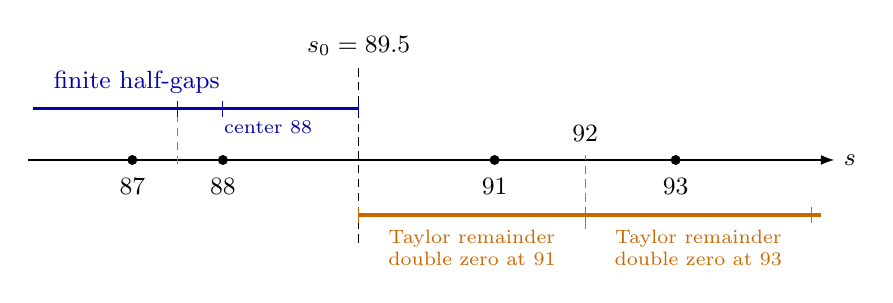
\begin{tikzpicture}[x=1.15cm,y=1cm,>=Latex,font=\small]
  \draw[->] (-.15,0) -- (8.75,0) node[right] {\(s\)};
  \foreach \a/\b in {1/87,2/88,5/91,7/93} {
    \fill (\a,0) circle (1.8pt);
    \node[below=3pt] at (\a,0) {\(\b\)};
  }
  \draw[densely dashed,gray] (1.5,-.05) -- (1.5,.72);
  \draw[densely dashed,gray] (6,-.88) -- (6,.06);
  \node[above=3pt] at (6,0) {\(92\)};
  \draw[densely dashed] (3.5,-1.05) -- (3.5,1.2);
  \node[above] at (3.5,1.2) {\(s_0=89.5\)};
  \draw[very thick,blue!65!black] (-.1,.65) -- (3.5,.65);
  \draw[blue!65!black] (1.5,.55) -- (1.5,.75);
  \draw[blue!65!black] (2,.55) -- (2,.75);
  \draw[blue!65!black] (3.5,.55) -- (3.5,.75);
  \node[above,text=blue!65!black] at (1.05,.72)
    {finite half-gaps};
  \node[below,text=blue!65!black,font=\scriptsize] at (2.5,.62)
    {center 88};
  \draw[very thick,orange!80!black] (3.5,-.7) -- (8.6,-.7);
  \draw[orange!80!black] (3.5,-.8) -- (3.5,-.6);
  \draw[orange!80!black] (6,-.8) -- (6,-.6);
  \draw[orange!80!black] (8.5,-.8) -- (8.5,-.6);
  \node[below,text=orange!80!black,font=\scriptsize,align=center]
    at (4.75,-.77) {Taylor remainder\\double zero at 91};
  \node[below,text=orange!80!black,font=\scriptsize,align=center]
    at (7.25,-.77) {Taylor remainder\\double zero at 93};
\end{tikzpicture}
\caption{The finite inequalities cover the half-gaps through \(s_0\).
In the tail, 91 is a nearest node on \([89.5,92]\), then 93 on
\([92,94.5]\), and so on.  A double zero at the chosen node turns the uniform
second-derivative estimate into a quadratic remainder bound.}
\label{fig:sign-junction}
\end{figure}

\subsection{Quotients after subtracting values and slopes}

Recall the quotient \(\mathcal D_{m,2}\) introduced before the finite
polynomial rows in Section~\ref{sec:finite}.  For a twice continuously
differentiable function \(u\), Taylor's formula gives
\[
 \mathcal D_{m,2}u(s)
 =\frac{u(s)-u(m)-(s-m)u'(m)}{(s-m)^2}
 =\int_0^1(1-v)u''\bigl(m+v(s-m)\bigr)\,\dd v.
\]
The integral also gives the removable value at \(s=m\).  As before,
\(\mathcal D_{0,0}u=u\) at the origin.  On a prescribed half-gap \(s=m+yx\),
\(0\le x\le1\), the relevant quotient is
\begin{equation}\label{eq:deleted-slack}
 \mathcal D_{m,\nu}F_i(s)
 =\sigma_i\mathcal D_{m,\nu}H_i(s)
  +\delta_i\mathcal D_{m,\nu}T_k(s).
\end{equation}
For \(m>0\), \eqref{eq:exact-slack-jets} makes this equal to
\(F_i(s)/(s-m)^2\) away from the center.  The deletion is performed on each
function before any approximation is made, so a nonzero constant or linear
approximation error is never divided by \((s-m)^2\).

\paragraph{Moving from the exact lists to the reference lists.}
Their combined \(\ell^1\) distance is less than \(2\cdot10^{-8}\).  A unit
list has spectral variation at most 36, direct frequency modulus at most one,
and transformed bounds \(|\lambda|<3\), \(|z|<3\).  The transformed damping
has positive exponent \(\pi\Ima z\), so there is no exponential growth at
nonnegative radii.  Taylor's integral formula and the derivative estimates of
Section~\ref{sec:fourier} therefore give the following bound.  Each
\(H_i-H_i^{\mathrm{ref}}\) contains a direct error from one list and a
transformed error from the other.  The \(\ell^1\) norms of the two list
differences add to less than \(2\cdot10^{-8}\), so the larger of the two
kernel bounds controls the sum:
\begin{align}
 \sup_{s\text{ in the half-gap}}
 \left|\mathcal D_{m,\nu}(H_i-H_i^{\mathrm{ref}})(s)\right|
 &\le\frac{36}{\nu!}(2\cdot10^{-8})
       \max\{\pi^\nu,3(3\pi)^\nu\}\notag\\
 &<.00011.\label{eq:deleted-list-error}
\end{align}
For \(\nu=0\), this is the zeroth-derivative estimate.  For \(\nu=2\), the
factor \(1/2\) is \(\int_0^1(1-v)\,\dd v\), and the last comparison is the
scalar bound in \eqref{eq:scalar-error-budgets}.  No zero jet is required of
the reference function; only the exact slack uses \eqref{eq:exact-slack-jets}.

\paragraph{Replacing the reference quotient by its finite polynomial.}
The entire Taylor series gives, in both cases \(\nu=0,2\),
\[
 \sigma_i\mathcal D_{m,\nu}H_i^{\mathrm{ref}}(m+yx)
 =\sum_{r=0}^{\infty}
   \sigma_i\frac{y^r}{(r+\nu)!}
     (H_i^{\mathrm{ref}})^{(r+\nu)}(m)x^r.
\]
The rows \(l_{i,r}\) in \eqref{eq:bernstein-rows} replace the included
derivatives by quadrature.  We claim
\begin{equation}\label{eq:half-gap-polynomial-error}
 \sup_{0\le x\le1}
 \left|\sigma_i\mathcal D_{m,\nu}H_i^{\mathrm{ref}}(m+yx)
       -\sum_{r=0}^{40}l_{i,r}q(k)x^r\right|<.000001.
\end{equation}
For the included coefficients, Lemma~\ref{lem:quadrature-error} controls the
scaled moment of order \(r+\nu\).  The row above has the additional multiplier
\(y^{-\nu}\), whose absolute value is at most 4.  By
\eqref{eq:reference-norm}, the combined reference-list norm is less than
\(4.8<5\).  Summing the 41 coefficient errors therefore gives at most
\(41\cdot4\cdot5\cdot10^{-31}\).

For the omitted powers, put \(Y=|y|\) and \(l=41+\nu\).  Their total is at
most
\begin{equation}\label{eq:half-gap-series-tail}
 \frac{Y^{-\nu}36\cdot5}
 {l!\bigl(1-3\pi Y/(l+1)\bigr)}
 \left((\pi Y)^l+
 3\max_{1\le j\le6}
 e^{-\pi\Ima z(t_j)m}
       \bigl(\pi|z(t_{j-1})|Y\bigr)^l\right).
\end{equation}
Indeed, each direct derivative contributes a factor \(i\pi t\), and each
transformed derivative a factor \(i\pi z(t)\).  On
\([t_{j-1},t_j]\), both \(\Ima z(t)\) and \(|z(t)|\) decrease.  Thus the
right endpoint maximizes \(e^{-\pi\Ima z(t)m}\), while the left endpoint
bounds the largest frequency modulus, including the endpoint atoms.  For each
fixed frequency, the ratio of successive terms in the absolute
exponential series is at most \(3\pi Y/(l+1)<1\).  Summing this geometric
majorant and then integrating against total variation gives the displayed
denominator.  The factor \(36\cdot5\) bounds the combined spectral
variation of the reference inputs.

The scalar calculation in Appendix~\ref{sec:arithmetic} replaces the maximum
in \eqref{eq:half-gap-series-tail} by the larger sum over all six intervals.
For
\[
 (m,Y,\nu)=(0,1/2,0),\quad(1,1,2),\quad(3,1,2),\quad(4,3/2,2),
\]
it gives, respectively, upper bounds \(1.8\cdot10^{-19}\), \(10^{-11}\),
\(3\cdot10^{-16}\), and \(2\cdot10^{-11}\), all below \(10^{-8}\).  These
four cases cover every half-gap.  The origin is the first case; the largest
half-lengths at 1 and 3 are one; and every later center is at least 4 with
half-length at most \(3/2\).  For fixed \(\nu\), the expression decreases as
\(m\) increases or \(Y\) decreases: its powers contain \(Y^{l-\nu}=Y^{41}\),
and the positive geometric denominator also improves when \(Y\) decreases.
Adding the included quadrature error proves
\eqref{eq:half-gap-polynomial-error}.

\subsection{Lower supports for every target regime}

\begin{lemma}[Exponential supports]\label{lem:exponential-support}
Let \(K,J\) be consecutive endpoints of the parameter partition in
Section~\ref{sec:finite}, and let \(K\le k\le J\), with no upper restriction
when \(J=\infty\).  On every prescribed half-gap, the coefficients \(a_r^*\)
from \eqref{eq:target-support} satisfy
\[
 \mathcal D_{m,\nu}T_k(m+yx)
 \ge\sum_{r=0}^{40}a_r^*x^r-.000001\qquad(0\le x\le1).
\]
\end{lemma}

\begin{proof}
At the origin, \(0\le s\le1/2\), and
\[
 \frac{\partial T_k(s)}{\partial k}
 =T_k(s)\left(1-s-\frac1k\right)>0
\]
because \(k\ge2.36>2\).  Replacing \(k\) by \(K\) therefore lowers the
target.  The Taylor polynomial of \(T_K(yx)\) through degree 40 has
coefficients \((e^K/K)(-Ky)^r/r!\), exactly the first case in
\eqref{eq:target-support}.

At the first positive node, write \(u=s-1\).  The deleted quotient is
\[
 \mathcal D_{1,2}T_k(1+u)=\frac{e^{-ku}-1+ku}{ku^2},
\]
with value \(k/2\) at \(u=0\).  For \(u\ne0\), its derivative with respect to
\(k\) is
\[
 \frac{1-(1+ku)e^{-ku}}{k^2u^2}\ge0,
\]
by \(e^{ku}\ge1+ku\).  The same monotonicity holds at the removable value.
This works for both signed half-gaps, including negative \(u\).  Replacing
\(k\) by \(K\) again lowers the quotient, and its Taylor coefficients are
\(K(-Ky)^r/(r+2)!\), the second case in \eqref{eq:target-support}.

In both cases the left endpoint satisfies \(K\le6\), even for the last,
unbounded parameter interval.  At the origin \(K|y|\le3\), and at node 1
\(K|y|\le6\).  Also \(e^K/K\) increases for \(K>1\), so its value is at most
\(e^6/6\).  The absolute tails after degree 40 are bounded by
\[
 \frac{e^6}{6}\frac{3^{41}}{41!(1-3/42)}<8\cdot10^{-29}<10^{-6},
 \qquad
 \frac{6\cdot6^{41}}{43!(1-6/44)}<10^{-20}<10^{-6},
\]
using the scalar comparisons in Appendix~\ref{sec:arithmetic}.  Thus no
Taylor estimate with unbounded \(k\) is needed.

At every positive node, Taylor's integral formula also gives the general
nonnegative support
\begin{equation}\label{eq:target-integral-quotient}
 \mathcal D_{m,2}T_k(m+u)
 =k\int_0^1(1-v)e^{-k(m-1+vu)}\,\dd v\ge0.
\end{equation}
This handles all cases in which \eqref{eq:target-support} prescribes zero.
It remains to justify the stronger constant at \(m=3\) for finite \(J\).
Here \(-1\le u\le1/2\), so \(a=2+vu\ge1\).  The function \(k e^{-ak}\)
decreases for \(k\ge2.36\), and \eqref{eq:target-integral-quotient} is at least
\[
 J\int_0^1(1-v)e^{-J(2+vu)}\,\dd v.
\]
The probability density \(2(1-v)\) on \([0,1]\) has mean \(1/3\).  Jensen's
inequality for the exponential therefore bounds this expression below by
\[
 \frac J2e^{-J(2+u/3)}\ge\frac J2e^{-13J/6},
\]
which is the third case of \eqref{eq:target-support}.  When \(J=\infty\), the
prescribed support is zero and \eqref{eq:target-integral-quotient} applies.
\end{proof}

\subsection{The bounded radial range}

\begin{lemma}[Signs on the finite half-gaps]\label{lem:half-gap-signs}
For every real \(k\ge2.36\), the exact slacks satisfy \(F_i(s)\ge0\) for
\(0\le s\le s_0\), \(i=1,2\).
\end{lemma}

\begin{proof}
Choose a half-gap and a parameter interval containing \(k\).  Combine the
finite rows and the target support into
\[
 \Phi_i(x;k)=\sum_{r=0}^{40}
       \bigl(l_{i,r}q(k)+\delta_i a_r^*\bigr)x^r.
\]
By the Bernstein conversion defining \eqref{eq:bernstein-rows}, the
coefficient of the \(d\)-th degree-40 Bernstein basis function is
\[
 L_{i,d}q(k)+\delta_i\sum_{r=0}^d\omega_{dr}a_r^*.
\]
The containing-box lower evaluation \eqref{eq:box-lower} applies to the
physical vector \(q(k)\).  Together with
Proposition~\ref{prop:finite-certificate}, it makes every coefficient above
strictly greater than \(.001\).  The Bernstein basis functions are
nonnegative and sum to one on \([0,1]\), so \(\Phi_i(x;k)>.001\) on that
entire interval.

Apply \eqref{eq:deleted-list-error},
\eqref{eq:half-gap-polynomial-error}, and
Lemma~\ref{lem:exponential-support} to \eqref{eq:deleted-slack}.  The result is
the strict quotient margin
\[
 \mathcal D_{m,\nu}F_i(m+yx)
 >.001-.00011-.000001-.000001=.000888>0.
\]
At the origin this is the desired inequality.  At a positive center,
multiplication by \((s-m)^2\) proves the inequality away from the center, and
\eqref{eq:exact-slack-jets} supplies equality at the center.  The half-gaps
cover \([0,s_0]\), while the five parameter intervals cover every finite
\(k\ge2.36\).
\end{proof}

\subsection{The tail and its quadratic scale}

Beyond \(s_0\), the low-node rational part of each direct cardinal function
has a positive signed value.  We will group the high-node terms, the
transformed function, and the target into a single remainder.  That sum has
a small second derivative and exact double zeros; its individual terms need
not have zero jets.  The following geometric bound lets us compare the
positive part and the remainder on the same squared-distance scale.

\begin{lemma}[Quadratic barrier for the sine product]
\label{lem:sine-product-barrier}
For every real \(s\), let \(m\in\mathcal Z\) be any nearest point of the full
periodic zero set, so \(|s-m|=\min_{n\in\mathcal Z}|s-n|\).  Then
\begin{equation}\label{eq:P-quadratic-lower}
 P(s)\ge .68(s-m)^2.
\end{equation}
\end{lemma}

\begin{proof}
The set \(\mathcal Z\) is discrete and periodic, so a nearest point exists.
Between a zero \(m\) and either adjacent midpoint, the quotient
\(P(s)/(s-m)^2\) is positive after its removable value is filled in.  Its
logarithm is concave.  For the factor vanishing at \(m\), with \(u=s-m\),
\[
 \frac{\dd^2}{\dd u^2}
 \log\left(\frac{\sin^2(\pi u/12)}{u^2}\right)
 =\frac2{u^2}-2\left(\frac\pi{12}\right)^2
                \csc^2\left(\frac{\pi u}{12}\right)\le0
\]
for \(u\ne0\), by \(|\sin x|\le|x|\), and the inequality extends through
the removable value.  Every other sine factor has nonpositive logarithmic
second derivative on this half-gap.  A concave function is bounded below by
the smaller of its endpoint values, so the quotient is bounded below by its
smaller value at the center and the midpoint.

At the center, the periodicity of \(P\) reduces the removable value to the
corresponding node value \(Q_n>1.75\) in \eqref{eq:node-constant-bounds}.  At
the midpoints, the exact values are
\[
\begin{array}{c|c}
 \text{gap modulo }12&P(s)/(s-m)^2\text{ at its midpoint}\\ \hline
 {[0,1],\ [3,4]}&12-8\sqrt2\\
 {[1,3]}&1\\
 {[4,7],\ [9,12]}&\dfrac89(3+\sqrt2+\sqrt3+\sqrt6)\\
 {[7,9]}&9
\end{array}
\]
Here the denominator is the square of the half-gap length, independent of
which endpoint is chosen at a tie.  For clarity, the smallest entry can be
derived directly.  At \(s=1/2\), put \(\theta=\pi/24\) and pair the unsquared
factors for residues \((1,7)\), \((3,9)\), and \((0,4)\).  Product-to-sum
gives
\begin{align*}
 (2\sin(-\theta))(2\sin(-13\theta))&=2\sin(\pi/12),\\
 (2\sin(-5\theta))(2\sin(-17\theta))&=2\sin(5\pi/12),\\
 (2\sin\theta)(2\sin(-7\theta))&=1-\sqrt2.
\end{align*}
The product of the first two right sides is one.  Thus
\(P(1/2)/(1/2)^2=4(1-\sqrt2)^2=12-8\sqrt2\).  The same product-to-sum
calculation at the other midpoints gives the remaining entries.  The identity
\(P(4-s)=P(s)\), which follows from invariance of \(L\) under
\(a\mapsto4-a\) modulo 12, accounts for the paired gap types in the table.
The smallest entry satisfies \(12-8\sqrt2>.6862>.68\), as recorded in
Appendix~\ref{sec:arithmetic}; every other entry is larger than \(.68\) as
well.  The half-gaps cover the real line, proving the claim, including the
zero values themselves.
\end{proof}

\begin{lemma}[Signs in the tail]\label{lem:tail-signs}
For every real \(k\ge2.36\), the exact slacks satisfy \(F_i(s)\ge0\) for
\(s\ge s_0\), \(i=1,2\).
\end{lemma}

\begin{proof}
We first bound the low-node rational contribution, then compare the remaining
term on the same quadratic scale.

\paragraph{The low-node rational part.}
Separate each direct cardinal function as
\begin{align*}
 R_{i,0}(s)
 &=C_i+\sum_{\substack{n\in\mathcal N_0\\n\le88}}
       \left(\frac{c_{in}}{(s-n)^2}+\frac{d_{in}}{s-n}\right),\\
 p_i(s)&=P(s)R_{i,0}(s)+p_{i,\mathrm{high}}(s).
\end{align*}
The high function contains precisely the node columns beginning at 91 and no
constant column.  Every denominator in \(R_{i,0}\) is positive for
\(s\ge s_0\).  We claim
\begin{equation}\label{eq:tail-rational-positive}
 \sigma_iR_{i,0}(s)>.002\qquad(s\ge s_0).
\end{equation}
For the reference lists, use the decomposition preceding
\eqref{eq:tail-certificate}, which groups the simple-pole rows into their
common \(1/s\) numerator before taking negative parts.  In the parameter
box containing \(k\), each numerator row \(l\) has the nonpositive lower
bound \(\eta_{K,J}(l)=\min(0,[l]_{K,J})\).  The reciprocal factors are
nonnegative and nonincreasing for \(s\ge s_0\), so their products with these
lower bounds give a value
at least as large as at \(s_0\); the constant row retains its full lower
bound \([C_i^*]_{K,J}\).  Thus \eqref{eq:tail-certificate} gives
\(\sigma_iR_{i,0}^{\mathrm{ref}}(s)>.0021\).

The passage to the exact list changes this rational function by less than
\(2\cdot10^{-8}\).  Indeed, \(s-n\ge1.5\) for every low node, so both
reciprocal coefficient factors have modulus at most one, as does the constant
factor; apply the full-list correction in \eqref{eq:exact-list-bounds}.
Since \(.0021-2\cdot10^{-8}>.002\), this proves
\eqref{eq:tail-rational-positive}.

\paragraph{The high-node list and the remainder.}
For the exact pair define the coupled input sizes
\[
 w=\sum_{i=1}^2\sum_{n\in\mathcal N_0}(|c_{in}|+|d_{in}|),\qquad
 c=\sum_{i=1}^2|C_i|.
\]
The full-list norm and the fixed extras give \(w+c<5\) and \(c<.02\), by
\eqref{eq:exact-list-bounds} and \eqref{eq:extra-constant-bound}.  At every
node \(n\ge91\), the exact equations
\eqref{eq:infinite-interpolation-system} read
\[
 (c_{1n},d_{1n})=(S\ell_2)_n+(\mathcal JT_k)_n,
 \qquad
 (c_{2n},d_{2n})=(S\ell_1)_n.
\]
Here \(S\ell_i=-\mathcal JK_{p_i}\) includes all input coordinates,
including the extras.  Applying Lemma~\ref{lem:kernel-bounds} to both lists
with their summed input bounds \(w,c\), the combined high-node norm is at
most \(U_{91}(w,c)\) plus the target geometric majorant
\[
 \frac{1+(1+2.12)/2.36}{1.75}
       \frac{e^{-2.36\cdot90}}{1-e^{-2.36}}<10^{-89}.
\]
This follows from \eqref{eq:target-jet-bound} by overcounting with all integers
from 91; the last comparison is the local calculation
\eqref{eq:target-tail-91}.  The finer scalar bound in
\eqref{eq:scalar-error-budgets} is \(U_{91}(5,.02)<2.2711\cdot10^{-7}\).
Since \(U_{91}\) is increasing in both input bounds, we obtain
\[
 \sum_{i=1}^2\sum_{\substack{n\in\mathcal N\\n\ge91}}
       (|c_{in}|+|d_{in}|)
 <2.2711\cdot10^{-7}+10^{-89}<2.4\cdot10^{-7}.
\]
The difference between \(2.2711\cdot10^{-7}\) and
\(2.4\cdot10^{-7}\) leaves room for this target contribution.

Define
\[
 Z_i(s)=\sigma_i\bigl(p_{i,\mathrm{high}}(s)+K_{p_{3-i}}(s)\bigr)
                  +\delta_iT_k(s).
\]
Then
\begin{equation}\label{eq:tail-decomposition}
 F_i(s)=\sigma_iP(s)R_{i,0}(s)+Z_i(s).
\end{equation}
We have the uniform bound
\begin{equation}\label{eq:tail-second-derivative}
 \sup_{s\ge s_0}|Z_i''(s)|<.0002.
\end{equation}
To verify it, the direct high columns contribute at most
\(36\pi^2(2.4\cdot10^{-7})\).  For the low-frequency transformed term, the
actual coupled full-list norm gives the important estimate
\[
 25c+36w\le36(c+w)<180.
\]
Thus the \([0,5/6]\) variation in \eqref{eq:refined-derivative-bound}, which
includes the atom at \(5/6\), is bounded by \(36\cdot5\).  On \((5/6,1]\),
we may separately use \(w<5\) and \(c<.02\); the only atom there is at 1 and
contributes \(2c<.04\).  Finally, \(T_k''(s)=k e^{-k(s-1)}\).  Its supremum
over \(s\ge s_0\), \(k\ge2.36\), occurs at \(s=s_0\), \(k=2.36\), since
\(s_0-1>1/2.36\).  The resulting four-term bound is
\begin{align*}
 &36\pi^2(2.4\cdot10^{-7})
  +3(3\pi)^2\,36\cdot5\,e^{-.70s_0}\\
 &\quad+1.25(1.32\pi)^2
       \left(\frac{2.54\cdot5}{s_0}+.04\right)e^{-.187s_0}
  +2.36e^{-2.36(s_0-1)}
 <8.5485\cdot10^{-5}<.0002,
\end{align*}
by the scalar comparison in Appendix~\ref{sec:arithmetic}.  This proves
\eqref{eq:tail-second-derivative}.

At every node \(m\in\mathcal N\) with \(m\ge91\), \(R_{i,0}\) is regular and
\(P\) has a double zero.  Subtracting its product from the exact slack jets
in \eqref{eq:tail-decomposition} therefore gives
\begin{equation}\label{eq:tail-remainder-jets}
 Z_i(m)=Z_i'(m)=0\qquad(m\in\mathcal N,\ m\ge91).
\end{equation}
These zeros use the exact interpolation equations, not merely the small norm
of the high list.

\paragraph{Comparison at a nearest zero.}
For \(s\ge s_0\), choose a nearest point \(m\in\mathcal Z\) with \(m\ge91\).
Such a choice is possible throughout the tail; at \(s=s_0\), choose 91 from
the tied points 88 and 91.  The segment joining \(s\) and \(m\) stays in
\([s_0,\infty)\).  Taylor's integral formula, using
\eqref{eq:tail-second-derivative} and \eqref{eq:tail-remainder-jets}, gives
\[
 |Z_i(s)|\le .0001(s-m)^2.
\]
On the other hand, \eqref{eq:tail-rational-positive} and
Lemma~\ref{lem:sine-product-barrier} imply
\[
 \sigma_iP(s)R_{i,0}(s)\ge .68\cdot.002(s-m)^2.
\]
Since \(.68\cdot.002>.0001\), \eqref{eq:tail-decomposition} gives
\(F_i(s)\ge0\).  At a node the exact zero value gives the same conclusion,
without division by a vanishing factor.
\end{proof}

\begin{proof}[Proof of Theorem~\ref{thm:normalized-pair}]
For every real \(k\ge2.36\), Proposition~\ref{prop:exact-interpolation}
supplies real summable lists with the prescribed extras.  Section~\ref{sec:fourier}
makes \(H_1,H_2\) entire and real on the real axis, and
Lemma~\ref{lem:fourier-pair} gives the real radial Schwartz Fourier pair
\[
 f(x)=e^{-\pi hb|x|^2}H_1(b|x|^2),\qquad
 \widehat f(\xi)=e^{-\pi hb|\xi|^2}H_2(b|\xi|^2).
\]
Lemmas~\ref{lem:half-gap-signs} and \ref{lem:tail-signs} cover all \(s\ge0\),
so \(H_1(s)\le T_k(s)\) and \(H_2(s)\ge0\).  The exact jets are
\[
 H_1(n)=T_k(n),\qquad H_1'(n)=T_k'(n),\qquad
 H_2(n)=H_2'(n)=0\qquad(n\in\mathcal N).
\]
This proves the theorem.
\end{proof}

\section{From Gaussian pairs to energy comparisons}
\label{sec:energy}

The preceding sections construct the Fourier pair in
Theorem~\ref{thm:normalized-pair}.  We now turn that pair into a sharp energy
bound for every Gaussian.  Two steps are needed.  First, Fourier nonnegativity
gives a lower bound for any locally finite configuration with the stated
centered density.  Second, scaling and Fourier complementation turn the
normalized pair into a minorant for every positive Gaussian parameter.
Section~\ref{sec:mixtures} then completes the universal-energy theorem by
positive mixtures. The renormalized and jellium consequences are treated
separately in Section~\ref{sec:renormalized}.

\subsection{An area comparison under centered density}

Recall that $B_R$ is the centered closed disk,
$\mathcal C_R=\mathcal C\cap B_R$, and $N_R=\#\mathcal C_R$.
The only geometric limit used below is $N_R/(\pi R^2)\to1$.
The density-only linear-programming argument is due to
Cohn and de~Courcy-Ireland~\citep[Proposition~2.2]{CohnDeCourcyIreland2018}, whose background-measure
comparison follows Cohn and Zhao~\citep[Theorem~3.3]{CohnZhao2014}.  The latter is a packing
theorem; its exclusion-distance hypothesis is not an assumption here.
We give the argument for the exact auxiliary class used in this paper.

\begin{proposition}[Linear programming with centered disk density]
\label{prop:density-lp}
Let $f$ be a real even Schwartz function on $\R^2$ whose Fourier transform is
nonnegative.  Every locally finite configuration $\mathcal C\subset\R^2$
with centered disk density one satisfies
\begin{equation}\label{eq:density-lp}
 \liminf_{R\to\infty}\frac1{N_R}
 \sum_{\substack{x,y\in\mathcal C_R\\x\ne y}}f(x-y)
 \ge \widehat f(0)-f(0).
\end{equation}
The same lower bound holds if $f(x-y)$ is replaced by $\Phi(x-y)$, where
$\Phi:\R^2\setminus\{0\}\to[0,\infty)$ satisfies $\Phi(z)\ge f(z)$.
\end{proposition}

\begin{proof}
For finite real signed measures $\mu,\nu$ on $\R^2$, define
\[
 Q(\mu,\nu)=\iint f(x-y)\,\dd\mu(x)\,\dd\nu(y),
 \qquad
 \widehat\mu(\xi)=\int e^{-2\pi i x\cdot\xi}\,\dd\mu(x).
\]
Fourier inversion and Fubini's theorem give
\[
 Q(\mu,\nu)=\int_{\R^2}\widehat f(\xi)
       \overline{\widehat\mu(\xi)}\widehat\nu(\xi)\,\dd\xi.
\]
Indeed, $\widehat f$ is integrable and the transforms of finite measures are
bounded.  Since $\widehat f\ge0$, this is a positive-semidefinite form and
therefore satisfies Cauchy--Schwarz.

Put $a=\widehat f(0)=\int f\ge0$ and
$\mu_R=\sum_{x\in\mathcal C_R}\delta_x$.  If $a=0$, positivity gives
$Q(\mu_R,\mu_R)/N_R\ge a$ whenever $N_R>0$.  Suppose now that $a>0$.
Fix $\varepsilon>0$ and let
\[
 \nu_R=1_{B_{(1+\varepsilon)R}}\,\dd x,
 \qquad V_R=\pi(1+\varepsilon)^2R^2.
\]
For every $x\in B_R$, the disk $B_{(1+\varepsilon)R}-x$ contains
$B_{\varepsilon R}$.  Thus
\begin{equation}\label{eq:uniform-cross-term}
 \bigl|Q(\mu_R,\nu_R)-N_Ra\bigr|
 \le N_R\int_{|z|\ge\varepsilon R}|f(z)|\,\dd z=o(N_R).
\end{equation}
The estimate is uniform in the locations of all points of $\mathcal C_R$;
it does not use a bound on their number in any smaller disk.

\begin{figure}[tb]
\centering
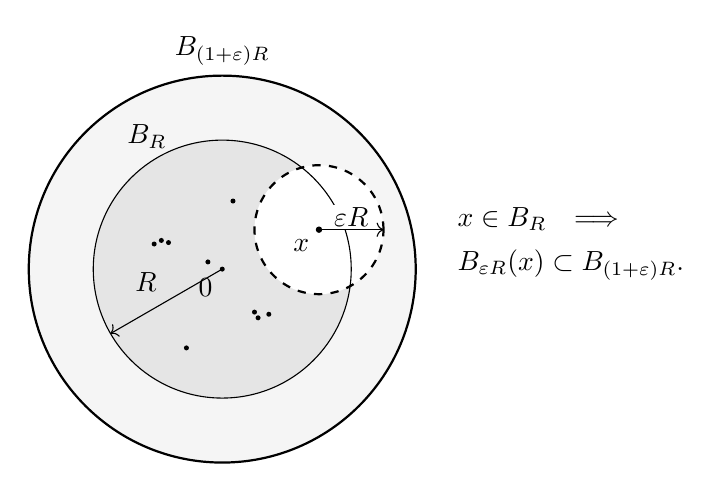
\begin{tikzpicture}[scale=.91]
 \fill[black!4] (0,0) circle (2.7);
 \fill[black!10] (0,0) circle (1.8);
 \fill[white] (1.35,.55) circle (.9);
 \draw[thick] (0,0) circle (2.7);
 \draw (0,0) circle (1.8);
 \draw[dashed,thick] (1.35,.55) circle (.9);
 \foreach \p in {(-.95,.35),(-.85,.4),(-.75,.37),(-.5,-1.1),
                  (.15,.95),(.45,-.6),(.5,-.68),(.65,-.63),(-.2,.1)}
   \fill \p circle (.035);
 \fill (0,0) circle (.035) node[below left] {$0$};
 \fill (1.35,.55) circle (.045) node[below left] {$x$};
 \draw[->] (0,0)--(-1.56,-.9)
   node[midway,above left] {$R$};
 \draw[->] (1.35,.55)--(2.25,.55)
   node[midway,above,fill=white,inner sep=1pt] {$\varepsilon R$};
 \node at (0,3.04) {$B_{(1+\varepsilon)R}$};
 \node at (-1.05,1.85) {$B_R$};
 \node[align=left,anchor=west] at (3.15,.35)
   {$x\in B_R$\quad$\Longrightarrow$\\[4pt]
    $B_{\varepsilon R}(x)\subset B_{(1+\varepsilon)R}$.};
\end{tikzpicture}
\caption{The comparison disk contains a disk of radius $\varepsilon R$
 around every $x\in\mathcal C_R$.  This containment gives the uniform tail
 error in \eqref{eq:uniform-cross-term}, including for clustered points.}
\label{fig:larger-disk}
\end{figure}

\Needspace{12\baselineskip}
The area self-term has the limit
\[
 \frac{Q(\nu_R,\nu_R)}{V_R}
 =\int_{\R^2}f(z)
   \frac{|B_{(1+\varepsilon)R}\cap(B_{(1+\varepsilon)R}-z)|}{V_R}
   \,\dd z
 \longrightarrow a.
\]
For each fixed $z$, the overlap fraction tends to one and is between zero
and one.  Dominated convergence therefore applies with dominator $|f|$.
In particular, $Q(\nu_R,\nu_R)>0$ for all sufficiently large $R$.
Cauchy--Schwarz and \eqref{eq:uniform-cross-term} now yield
\[
 \frac{Q(\mu_R,\mu_R)}{N_R}
 \ge\frac{|Q(\mu_R,\nu_R)|^2}{N_RQ(\nu_R,\nu_R)}
 =\frac{N_R}{V_R}\frac{(a+o(1))^2}{a+o(1)}.
\]
Since $N_R/V_R\to(1+\varepsilon)^{-2}$, taking the lower limit in $R$
and then letting $\varepsilon\downarrow0$ proves
\[
 \liminf_{R\to\infty}\frac{Q(\mu_R,\mu_R)}{N_R}\ge a.
\]
There are exactly $N_R$ diagonal terms, each equal to $f(0)$, so removing
them proves \eqref{eq:density-lp}.  The assertion for $\Phi$ follows by
termwise comparison of each finite off-diagonal sum.
\end{proof}

\FloatBarrier

\subsection{Sharp pairs for every Gaussian parameter}

The normalized theorem directly covers $\alpha\ge1$.
Fourier complementation supplies $0<\alpha<1$.  This is the Gaussian form
of the duality in Cohn and Miller~\citep[Section~6]{CohnMiller2016}; we give the calculation
to fix the dimension-two factor and the two contact sets.

\begin{lemma}[Gaussian duality]\label{lem:gaussian-duality}
For every $\alpha>0$, let $G_\alpha(x)=e^{-\pi\alpha|x|^2}$.
There is a real radial Schwartz function $f_\alpha$ such that, pointwise,
\begin{equation}\label{eq:gaussian-sharp-pair}
 \begin{gathered}
 f_\alpha\le G_\alpha,\qquad \widehat f_\alpha\ge0,\\
 f_\alpha(a)=G_\alpha(a)\quad(a\in A\setminus\{0\}),\qquad
 \widehat f_\alpha(w)=0\quad(w\in A^*\setminus\{0\}).
 \end{gathered}
\end{equation}
\end{lemma}

\begin{proof}
For $\alpha\ge1$, take
\[
 k=\pi(\alpha/b-h)\ge\pi(2/\sqrt3-2/5)>2.36.
\]
The elementary comparison is proved in Appendix~\ref{sec:arithmetic}.
Let $f$ be the function supplied by Theorem~\ref{thm:normalized-pair}
for this $k$, and define $f_\alpha=ke^{-k}f$.  The multiplier is positive,
so $\widehat f_\alpha\ge0$.  With $s=b|x|^2$, the upper bound for
$f_\alpha$ becomes
\[
 ke^{-k}e^{-\pi hs}T_k(s)
 =e^{-(\pi h+k)s}=e^{-\pi\alpha|x|^2}.
\]
The shell containment and $A^*=JA$ from Section~\ref{sec:fourier} place every
nonzero direct and dual shell in $\mathcal N$.  The value contacts in
\eqref{eq:normalized-jets} therefore give \eqref{eq:gaussian-sharp-pair}.

For $0<\alpha<1$, put $\beta=1/\alpha$ and use the function already
constructed for $\beta>1$.  Define its nonnegative radial Schwartz slacks
\[
 q_\beta=G_\beta-f_\beta,\qquad r_\beta=\widehat f_\beta.
\]
The Fourier transform applied twice is reflection, which is immaterial for
these radial functions.  Thus $G_\beta=q_\beta+\widehat r_\beta$.
The dimension-two Gaussian transform from
\eqref{eq:complex-gaussian-transform} gives
\[
 \beta^{-1}G_\alpha=\widehat G_\beta
 =\widehat q_\beta+r_\beta.
\]
Set
\begin{equation}\label{eq:reciprocal-minorant}
 f_\alpha=\beta\widehat q_\beta.
\end{equation}
Then $G_\alpha-f_\alpha=\beta r_\beta\ge0$ and
$\widehat f_\alpha=\beta q_\beta\ge0$.  The known contacts say that
$q_\beta$ vanishes on $A\setminus\{0\}$ and $r_\beta$ vanishes on
$A^*\setminus\{0\}$.  Since $A^*$ is a rotation of $A$ and both functions
are radial, $q_\beta$ also vanishes on the nonzero dual shells and
$r_\beta$ on the nonzero direct shells.  The two displayed slack identities
give the required contacts for $f_\alpha$.
\end{proof}

It remains to identify the lower bound with the Gaussian lattice sum.
Periodize the fixed Schwartz function $f_\alpha$ over $A$.  Schwartz decay
makes the periodization smooth, and termwise integration over a unit-area
fundamental cell gives Fourier coefficients $\widehat f_\alpha(w)$ for
$w\in A^*$.  These coefficients are absolutely summable.  Evaluating the
Fourier series at zero gives
$\sum_{a\in A}f_\alpha(a)=\sum_{w\in A^*}\widehat f_\alpha(w)$.
Using \eqref{eq:gaussian-sharp-pair} and removing the origin yields
\begin{equation}\label{eq:gaussian-lattice-value}
 \sum_{a\in A\setminus\{0\}}G_\alpha(a)
 =\widehat f_\alpha(0)-f_\alpha(0).
\end{equation}
Only the lattice has been periodized; no periodicity is assumed of the
competitor.  Proposition~\ref{prop:density-lp} with $\Phi=G_\alpha$ therefore
proves, for every locally finite $\mathcal C$ of centered disk density one
and every $\alpha>0$,
\begin{equation}\label{eq:gaussian-energy}
 \liminf_{R\to\infty}\frac1{N_R}
 \sum_{\substack{x,y\in\mathcal C_R\\x\ne y}}
 e^{-\pi\alpha|x-y|^2}
 \ge\sum_{a\in A\setminus\{0\}}e^{-\pi\alpha|a|^2}.
\end{equation}
This scalar inequality is the input for the positive-mixture argument in the
next section.  No measurable choice of the functions $f_\alpha$ will be
needed there.

\section{Shifted moments and positive mixtures}
\label{sec:mixtures}

Equation~\eqref{eq:gaussian-energy} compares the configuration with the
triangular lattice for every kernel $e^{-\pi\alpha t}$.  To pass to a
completely monotone interaction, we represent it by positive mixtures of
these kernels.  A potential may be singular at zero, so a finite representing
measure need not be available for the unshifted function.  We instead
construct one for each positive shift and remove the shift only after taking
the lattice sum.

\subsection{A finite moment representation}

The representation belongs to the classical Hausdorff--Bernstein--Widder
theory \citep{Hausdorff1921,Bernstein1929,Widder1931}.  We prove precisely the
finite-measure form needed here.  The construction first solves a discrete
moment problem using finite differences, then passes to all positive real
exponents.  It also identifies the endpoint masses that enter the energy
argument.

\begin{lemma}[Positive mixtures]\label{lem:positive-mixture}
Let $F:[0,\infty)\to[0,\infty)$ be smooth, with one-sided derivatives at
zero, and suppose $(-1)^jF^{(j)}(t)\ge0$ for every integer $j\ge0$ and every
$t\ge0$.  There is a finite positive Borel measure $\rho$ on $[0,1]$ of
total mass $F(0)$ such that
\begin{equation}\label{eq:positive-mixture}
 F(t)=\int_{[0,1]}v^t\,\dd\rho(v)\qquad(t>0).
\end{equation}
Moreover, $\rho(\{0\})=0$.  An atom at $1$ is allowed and contributes a
constant function.
\end{lemma}

\begin{proof}
\emph{Compactness of the measures.}
We first record an elementary compactness argument that preserves the limiting
total mass without discarding possible endpoint atoms.  Let $(\mu_n)$ be any
sequence of positive measures on $[0,1]$ with
uniformly bounded masses.  By a diagonal subsequence, arrange that the masses
converge to $m$ and that $\mu_n([0,q])$ converges to $a(q)$ for every rational
$q\in(0,1)$.  For $0\le x<1$, set
\[
 H(x)=\inf_{\substack{x<q<1\\q\text{ rational}}}a(q),
 \qquad H(1)=m.
\]
The function $H$ is nondecreasing and right-continuous.  Its associated
positive Borel measure $\mu$ has distribution $\mu([0,x])=H(x)$, including
mass $H(0)$ at zero and mass $m-H(1-)$ at one.  At every continuity point
$x\in(0,1)$ of $H$, rational points on either side of $x$ bracket
$\mu_n([0,x])$ and give convergence to $H(x)$.  Step-function approximations
on partitions with such internal endpoints, together with convergence of
the total masses and uniform continuity, then give
\[
 \int\varphi\,\dd\mu_n\longrightarrow\int\varphi\,\dd\mu
 \quad\text{for every continuous }\varphi:[0,1]\to\R.
\]
Thus the subsequence converges weakly.  The endpoint atoms have not been
discarded in this construction.

\emph{Discrete moments.}
Fix $d>0$ and put $m_j=F(jd)$ for integers $j\ge0$.
Writing $\Delta m_j=m_{j+1}-m_j$, repeated integration gives, for $r\ge1$,
\[
 (-1)^r\Delta^r m_j
 =\int_{[0,d]^r}(-1)^r F^{(r)}(jd+u_1+\cdots+u_r)
       \,\dd u_1\cdots\dd u_r\ge0.
\]
Define a linear functional on polynomials by $\Lambda(x^j)=m_j$.
For every integer $M\ge1$, place at $p/M$, $0\le p\le M$, the mass
\[
 w_{M,p}=\Lambda\!\left(\binom Mp x^p(1-x)^{M-p}\right)
 =\binom Mp(-1)^{M-p}\Delta^{M-p}m_p\ge0.
\]
Let $\mu_{M,d}=\sum_{p=0}^M w_{M,p}\delta_{p/M}$.  Its total mass is
$m_0$, because the Bernstein basis sums to one.  For fixed
$0\le j\le M$, the identity
$\binom Mp\binom pj=\binom Mj\binom{M-j}{p-j}$ gives
\[
 \sum_{p=0}^M\frac{\binom pj}{\binom Mj}
       \binom Mp x^p(1-x)^{M-p}=x^j.
\]
Applying $\Lambda$ shows that
$\sum_p w_{M,p}\binom pj/\binom Mj=m_j$.
For fixed $j$ and $M\ge\max\{1,j\}$, put
\[
 P_{M,j}(x)=\prod_{r=0}^{j-1}\frac{Mx-r}{M-r}.
\]
These polynomials converge uniformly to $x^j$ on $[0,1]$ as $M\to\infty$:
each of their finitely many factors converges uniformly to $x$.  At
$x=p/M$ their values are exactly $\binom pj/\binom Mj$, so the identity
above says $\int P_{M,j}\,\dd\mu_{M,d}=m_j$.  Since $\mu_{M,d}$ is
positive with mass $m_0$,
\[
 \left|\int x^j\,\dd\mu_{M,d}-m_j\right|
 \le m_0\|x^j-P_{M,j}\|_\infty\longrightarrow0.
\]
The compactness argument supplies one weakly convergent subsequence of
$(\mu_{M,d})_{M\ge1}$.  Since the moment convergence holds for every
fixed $j$ along the full sequence, its limit $\eta_d$ satisfies all the moment identities
\[
 F(jd)=\int_{[0,1]}x^j\,\dd\eta_d(x)
 \qquad(j=0,1,2,\ldots).
\]
In particular, $\eta_d$ has mass $F(0)$.

\emph{Positive real exponents.}
For each positive integer $l$, push $\eta_{1/l}$ forward by $x\mapsto x^l$
and call the resulting measure $\rho_l$.  It has mass $F(0)$ and
\[
 \int_{[0,1]}v^{j/l}\,\dd\rho_l(v)=F(j/l)
 \qquad(j=1,2,\ldots).
\]
Choose one weakly convergent subsequence $\rho_{l_n}\to\rho$; necessarily
$l_n\to\infty$, and the limit still has mass $F(0)$.
Now fix any $t>0$ and set $t_n=\lceil l_nt\rceil/l_n$.  Since
$0\le t_n-t<1/l_n$ and
$\sup_{0<v\le1}v^t|\log v|=1/(et)$, the mean value theorem in the exponent
gives the following bound; at $v=0$ both powers are zero because their
exponents are positive:
\[
 \sup_{0\le v\le1}|v^{t_n}-v^t|
 \le\frac{t_n-t}{et}\longrightarrow0.
\]
Continuity of $F$ and weak convergence against the continuous function $v^t$
now imply
\[
 F(t)=\lim_nF(t_n)
 =\lim_n\int v^{t_n}\,\dd\rho_{l_n}
 =\int v^t\,\dd\rho.
\]
The subsequence was chosen before $t$, so the same $\rho$ works for every
$t>0$.  Finally, as $t\downarrow0$, the functions $v^t$ increase to
$1_{(0,1]}(v)$.  Monotone convergence and continuity of $F$ at zero give
$\rho((0,1])=F(0)=\rho([0,1])$, proving $\rho(\{0\})=0$.
\end{proof}

\subsection{Lower limits and singular interactions}

The next proposition isolates the positive-mixture step.  Its Gaussian
hypothesis has already been proved for every configuration considered here
in \eqref{eq:gaussian-energy}.

\begin{proposition}[Positive-mixture transfer]\label{prop:energy-reduction}
Let $\mathcal C\subset\R^2$ be locally finite with centered disk density one.
Suppose that, for every $\alpha>0$,
\[
 \liminf_{R\to\infty}\frac1{N_R}
 \sum_{\substack{x,y\in\mathcal C_R\\x\ne y}}e^{-\pi\alpha|x-y|^2}
 \ge\sum_{a\in A\setminus\{0\}}e^{-\pi\alpha|a|^2}.
\]
Then every smooth completely monotone $g:(0,\infty)\to[0,\infty)$ satisfies
\begin{equation}\label{eq:full-energy-bound}
 E_g(\mathcal C)\ge\sum_{a\in A\setminus\{0\}}g(|a|^2)
\end{equation}
in the extended nonnegative reals, with the ordered-pair energy defined in
\eqref{eq:energy-definition}.
\end{proposition}

\begin{proof}
Fix $\varepsilon>0$ and set $F_\varepsilon(t)=g(\varepsilon+t)$ for $t\ge0$.
It satisfies Lemma~\ref{lem:positive-mixture}, with a finite representing
measure $\rho_\varepsilon$ of mass $g(\varepsilon)$.
Choose any real sequence $R_n\to\infty$, discarding finitely many terms so
that $N_{R_n}>0$, and define
\[
 A_n(v)=\frac1{N_{R_n}}
 \sum_{\substack{x,y\in\mathcal C_{R_n}\\x\ne y}}v^{|x-y|^2}
 \qquad(0\le v\le1).
\]
Every exponent is positive, so $A_n$ is continuous and nonnegative on
$[0,1]$, with $0^t=0$ for $t>0$.  Define the nonnegative extended-valued
function
\[
 L(v)=\sum_{a\in A\setminus\{0\}}v^{|a|^2}\qquad(0\le v\le1).
\]
For $0<v<1$, the Gaussian hypothesis with $\alpha=-\log(v)/\pi$ gives
\[
 \liminf_n A_n(v)\ge L(v).
\]
A full-radius lower-limit inequality holds along every sequence tending to
infinity.  The same comparison holds at the endpoints:
$A_n(0)=L(0)=0$, while
$A_n(1)=N_{R_n}-1\to\infty=L(1)$.

The finite-sum representation, Fatou's lemma, and Tonelli's theorem now give
\begin{align*}
 &\liminf_n\frac1{N_{R_n}}
   \sum_{\substack{x,y\in\mathcal C_{R_n}\\x\ne y}}
        F_\varepsilon(|x-y|^2)\\
 &\qquad=\liminf_n\int A_n(v)\,\dd\rho_\varepsilon(v)\\
 &\qquad\ge\int\liminf_n A_n(v)\,\dd\rho_\varepsilon(v)
 \ge\int L(v)\,\dd\rho_\varepsilon(v)\\
 &\qquad=\sum_{a\in A\setminus\{0\}}F_\varepsilon(|a|^2).
\end{align*}
Every integrand and summand is nonnegative, so these steps remain valid when
the last sum is infinite.  Since the sequence $R_n$ was arbitrary, this is
the full-radius lower bound for $F_\varepsilon$.

Complete monotonicity gives $g'\le0$, hence $g(t)\ge F_\varepsilon(t)$ for
$t>0$.  Termwise comparison therefore yields
\[
 E_g(\mathcal C)\ge
 \sum_{a\in A\setminus\{0\}}g(\varepsilon+|a|^2)
 \qquad(\varepsilon>0).
\]
As $\varepsilon\downarrow0$, the summands increase to $g(|a|^2)$.
Monotone convergence in the lattice sum proves \eqref{eq:full-energy-bound}.
No limit in $\varepsilon$ has been interchanged with the configuration lower
limit, and no unshifted representing measure has been used.
\end{proof}

\begin{proof}[Completion of the proof of Theorem~\ref{thm:universal}]
Equation~\eqref{eq:gaussian-energy} verifies the proposition's hypothesis
for every locally finite configuration of centered disk density one.  This
proves the inequality in Theorem~\ref{thm:universal}.  We finish by checking
attainment, including the case of an infinite lattice sum.

Choose a bounded half-open fundamental cell of $A$ with vertex zero and area one, and let
$d$ bound the distance of its points from its lattice vertex.  Up to boundary
sets of area zero, for $R>d$ the union of cells whose vertices lie in $A\cap B_R$
contains $B_{R-d}$ and is contained in $B_{R+d}$.  Its area is
$\#(A\cap B_R)$, so $A$ has centered disk density one.  For each
$x\in A\cap B_R$, the differences $y-x$ with
$y\in A\cap B_R\setminus\{x\}$ form a subset of $A\setminus\{0\}$.
Nonnegativity gives
\[
 \sum_{\substack{y\in A\cap B_R\\y\ne x}}g(|x-y|^2)
 \le\sum_{a\in A\setminus\{0\}}g(|a|^2).
\]
If the lattice sum is finite, averaging gives the upper bound for $E_g(A)$,
and \eqref{eq:full-energy-bound} applied to $A$ gives the reverse bound.
If the lattice sum is infinite, the same lower bound gives $E_g(A)=\infty$.
Thus the equality in Theorem~\ref{thm:universal} holds in every case.
\end{proof}

\section{Renormalized and jellium energies}
\label{sec:renormalized}

The universal-energy theorem is now proved. For the nonsummable Riesz
kernels with $0<s<2$ and for the logarithm, the meaningful finite comparison
comes from neutralizing the points against a uniform background and removing
their self-energy. Petrache and Serfaty established the implication from
universal optimality to these crystallization conclusions
\citep[Theorem~2]{PetracheSerfaty2020}. We give the transfer for the field
normalization and order of limits specified below.

The decisive intermediate comparison allows arbitrary period lattices.
Consequently the square-periodic approximation of the field infimum in
Appendix~\ref{app:normalized-periodic-approximation} suffices, although the
minimizing lattice is triangular.

\subsection{Field and scalar energy conventions}

Following the field-first construction of Petrache and Serfaty
\citep[Definitions~1.2--1.3]{PetracheSerfaty2017}, we define the energy
with its full-space normalization fixed by the fundamental-solution
equation below.  The truncation limit and cubic approximation for this
convention are established in
Proposition~\ref{prop:normalized-cubic-approximation}.
For $0\le s<2$, put
\[
 g_s(X)=\begin{cases}-\log|X|,&s=0,\\ |X|^{-s},&0<s<2,\end{cases}
 \qquad
 (k,\gamma)=\begin{cases}(0,0),&s=0,\\(1,s-1),&0<s<2.\end{cases}
\]
Write $X=(x,y)\in\R^2\times\R^k$, with the extra coordinate omitted
when $k=0$, and let $w_s=|y|^\gamma$ for $k=1$ and $w_0=1$.
The full-space identity
\[
 -\operatorname{div}(w_s\nabla g_s)=\kappa_s\delta_0
\]
gives $\kappa_0=2\pi$ and, for $0<s<2$,
\[
 \kappa_s=s\int_{S^2}|\omega_y|^{s-1}\,d\sigma(\omega)=4\pi.
\]
Here $\omega_y$ is the vertical coordinate on the unit sphere, and
$\delta_{\R^2}$ denotes area measure on $\R^2\times\{0\}$.

Fix once and for all $p$ with $1<p<2$ if $s=0$, and
\[
 1<p<\min\left(2,\frac2s,\frac3{s+1}\right)
 \qquad\text{if }0<s<2.
\]
For a locally finite configuration $\mathcal C$, admissible fields are
gradients $E=\nabla h$ in $L^p_{\mathrm{loc}}(\R^{2+k};\R^{2+k})$
with $w_sE\in L^1_{\mathrm{loc}}$, satisfying
\[
 -\operatorname{div}(w_sE)
 =\kappa_s\left(\sum_{p\in\mathcal C}\delta_{(p,0)}
                      -\delta_{\R^2}\right).
\]
This is the local integrability range following
Petrache and Serfaty~\citep[Definition~1.2]{PetracheSerfaty2017}.  Set
\[
 f_{s,\eta}=(g_s-g_s(\eta))_+,
 \qquad E_\eta=E-\sum_{p\in\mathcal C}
                       \nabla f_{s,\eta}(X-(p,0)).
\]
Thus the scalar potential subtracts $f_{s,\eta}$ and its gradient
subtracts $\nabla f_{s,\eta}$.  For $K_R=[-R/2,R/2]^2$, define
\begin{align*}
 \mathcal W_{s,\eta}(E)&=\limsup_{R\to\infty}
 \left[\frac1{R^2}\int_{K_R\times\R^k}w_s|E_\eta|^2
                         -\kappa_sg_s(\eta)\right],\\
 \mathcal W_s(E)&=\lim_{\eta\downarrow0}\mathcal W_{s,\eta}(E),
 \qquad W_s(\mathcal C)=\inf_E\mathcal W_s(E).
\end{align*}
The truncation limit exists in $\R\cup\{+\infty\}$ by
Proposition~\ref{prop:normalized-cubic-approximation}; the infimum is over
compatible admissible fields and is $+\infty$ if there are none.
In particular, the configuration infimum is outside both limits.

The periodic energy has the same field normalization.  For a torus
$T=\R^2/L$ of area $N\in\N$ and distinct points $a_1,\ldots,a_N$,
let $H$ be the canonical potential with mean-zero trace satisfying
\[
 -\operatorname{div}(w_s\nabla H)
 =\kappa_s\left(\sum_{i=1}^N\delta_{(a_i,0)}-\delta_T\right),
\]
with finite truncated energy on $T\times\R^k$.  Truncations include
the periodic images of the charges.  Set
\[
 W_{s,L}(a_1,\ldots,a_N)=\lim_{\eta\downarrow0}
 \left[\frac1N\int_{T\times\R^k}w_s|\nabla H_\eta|^2
                                      -\kappa_sg_s(\eta)\right].
\]
If $\mathcal G_L$ is the mean-zero unit-source extension Green function,
\[
 -\operatorname{div}(w_s\nabla\mathcal G_L)
      =\delta_{(0,0)}-N^{-1}\delta_T,
\]
integration by parts gives
\[
 W_{s,L}=\kappa_s^2\left[
  \frac1N\sum_{i\ne j}\mathcal G_L(a_i-a_j,0)
  +\lim_{x\to0}\left(\mathcal G_L(x,0)-\frac{g_s(x)}{\kappa_s}\right)
 \right].
\]
This follows the integration-by-parts argument of
Petrache and Serfaty~\citep[Proposition~1.5]{PetracheSerfaty2017}, using the Green function
and coefficient determined by the displayed extension equation.

For $N\in\N$, set $R=\sqrt N$ and $K_R=[-R/2,R/2]^2$.
The finite ordered-pair jellium energy is
\begin{equation}
\label{eq:finite-ordered-jellium}
\begin{split}
 J_{s,R}(a_1,\ldots,a_N)
 ={}&\sum_{i\ne j}g_s(a_i-a_j)
       -2\sum_{i=1}^N\int_{K_R}g_s(a_i-x)\,\dd x\\
    &+\int_{K_R}\int_{K_R}g_s(x-x')\,\dd x\,\dd x'.
\end{split}
\end{equation}
Here the particles are distinct; collisions have energy $+\infty$.
We use the density-one thermodynamic minimum
\[
 e_{\mathrm{Jel}}^{(s)}
 =\lim_{N\to\infty}\frac1N
       \min_{a_1,\ldots,a_N\in K_{\sqrt N}}
                    J_{s,\sqrt N}(a_1,\ldots,a_N).
\]
Since $|K_{\sqrt N}|=N$, normalization per particle and per unit area
coincide.  The scalar thermodynamic results and finite confinement
argument below establish the existence of this limit.

\subsection{The triangular minimum}

\begin{corollary}[Planar renormalized and jellium energies]
\label{cor:riesz-jellium}
Let $0\le s<2$.  For every positive integer $n$, put $N=n^2$ and
enumerate $A/(nA)$ by $a_1^\triangle,\ldots,a_N^\triangle$.
Every configuration of $N$ distinct points in $\R^2/(nA)$ satisfies
\[
 W_{s,nA}(a_1,\ldots,a_N)
 \ge W_{s,nA}(a_1^\triangle,\ldots,a_N^\triangle).
\]
Moreover, $A$ minimizes $W_s$ among density-one planar configurations,
and $e_{\mathrm{Jel}}^{(s)}=\kappa_s^{-1}W_s(A)$.
\end{corollary}

For a density-one periodic configuration $\mathcal C=\bigcup_{i=1}^N(a_i+L)$,
write $V_s(\mathcal C)=W_{s,L}(a_1,\ldots,a_N)$ for its canonical
periodic value. The following identity compares these values without
requiring the configurations to share a period lattice.

\begin{lemma}[Heat comparison across period lattices]
\label{lem:periodic-heat-comparison}
Let $0\le s<2$, and let $\mathcal C$ and $\mathcal D$ be simple periodic
configurations of density one. Put
\[
 q_0=2\pi,\qquad
 q_s=\frac{2^{2-s}\pi\Gamma(1-s/2)}{\Gamma(s/2)}\quad(0<s<2),
 \qquad \Psi_t(x)=(4\pi t)^{-1}e^{-|x|^2/(4t)}.
\]
If $\mathcal C=\bigcup_{i=1}^N(a_i+L)$, where $|\R^2/L|=N$, define
\[
 P_{t,L}(x)=\sum_{v\in L}\Psi_t(x-v),\qquad
 H_{\mathcal C}(t)=\frac1N\sum_{i,j=1}^N P_{t,L}(a_i-a_j)-\Psi_t(0),
\]
and define $H_{\mathcal D}$ using its own period lattice and point count.
Then the following integral is absolutely convergent and satisfies
\[
 V_s(\mathcal C)-V_s(\mathcal D)
 =\frac{\kappa_s q_s}{\Gamma(1-s/2)}\int_0^\infty
       \bigl(H_{\mathcal C}(t)-H_{\mathcal D}(t)\bigr)t^{-s/2}\,\dd t.
\]
\end{lemma}

\begin{proof}
Put $\alpha=1-s/2$. We first identify the scalar Green function whose
heat representation has the field normalization used here.
On the base plane, $(-\Delta)^\alpha g_s(\cdot,0)=q_s\delta_0$,
with the extra coordinate omitted when $s=0$.  On $T=\R^2/L$,
the spectral operator $(-\Delta)^\alpha$ multiplies the Fourier mode
$e^{2\pi i\xi\cdot x}$, $\xi\in L^*$, by $\lambda_\xi^\alpha$,
where $\lambda_\xi=(2\pi|\xi|)^2$.
Its mean-zero unit-source Green function $G_L$ therefore has coefficient
$N^{-1}\lambda_\xi^{-\alpha}$ for each $\xi\ne0$.
To compare it with the full-space extension, suppose first that $0<s<2$.
For $\lambda>0$, the even profile
\[
 u_\lambda(y)=\frac1{\Gamma(\alpha)}\int_0^\infty
 t^{\alpha-1}e^{-\lambda t-y^2/(4t)}\,\dd t
\]
decays at infinity and satisfies
\[
 u_\lambda(0)=\lambda^{-\alpha},\qquad
 u_\lambda''+\frac{1-2\alpha}{y}u_\lambda'-\lambda u_\lambda=0
 \quad(y>0).
\]
Differentiation and the substitution $v=y^2/(4t)$ give its full,
two-sided weighted flux:
\[
 -2\lim_{y\downarrow0}y^{1-2\alpha}u_\lambda'(y)
 =2^{2-2\alpha}\frac{\Gamma(1-\alpha)}{\Gamma(\alpha)}
 =\frac{\kappa_s}{q_s}.
\]
Thus the unit-source extension mode is
$(q_s/(N\kappa_s))u_{\lambda_\xi}$, whose trace is
$(q_s/\kappa_s)N^{-1}\lambda_\xi^{-\alpha}$.
The zero mode has no source: finite tail energy forces it to be
constant, and the mean-zero trace sets that constant to zero.
For $s=0$ there is no extension coordinate; both Green functions solve
$-\Delta G=\delta_0-N^{-1}$ on $T$ with zero mean, and
$q_0/\kappa_0=1$.  Hence, throughout $0\le s<2$,
$\mathcal G_L(x,0)=(q_s/\kappa_s)G_L(x)$, with the trace notation
omitted at $s=0$.  The periodic formula above consequently becomes
\[
 W_{s,L}=\kappa_sq_s\left[
  \frac1N\sum_{i\ne j}G_L(a_i-a_j)
  +\lim_{x\to0}\left(G_L(x)-\frac{g_s(x)}{q_s}\right)\right].
\]

Set
\[
 B_{\mathcal C}(t,x)=\frac1N\sum_{i,j}P_{t,L}(a_i-a_j+x),
\]
so $B_{\mathcal C}(t,0)=H_{\mathcal C}(t)+\Psi_t(0)$.
The heat representation \citep[Lemma~1]{PetracheSerfaty2020} is
\[
 G_L(x)=\frac1{\Gamma(\alpha)}\int_0^\infty
       \left(P_{t,L}(x)-\frac1N\right)t^{\alpha-1}\,\dd t.
\]
Its spectral proof applies to any flat torus.  To compare two periodic
configurations $\mathcal C$ and $\mathcal D$, set
$S_{\mathcal C}(x)=N^{-1}\sum_{i,j}G_L(a_i-a_j+x)$, and define
$S_{\mathcal D}$ using its own period lattice and point count.
Each $S$ has singular part $g_s(x)/q_s$.  In their heat-integrand
difference the background terms are both $1$ and the diagonal terms
are both $\Psi_t(x)$, so these terms cancel.  Uniformly for $x$ near
zero, the remaining difference is bounded by $Ct^{-1}e^{-c/t}$ as
$t\downarrow0$, because the other image distances are positive, and
by $Ce^{-\lambda t}$ as $t\to\infty$, by the two torus spectral gaps.
Dominated convergence as $x\to0$ consequently gives
\[
 V_s(\mathcal C)-V_s(\mathcal D)
 =\frac{\kappa_sq_s}{\Gamma(1-s/2)}\int_0^\infty
       \big(H_{\mathcal C}(t)-H_{\mathcal D}(t)\big)t^{-s/2}\,\dd t.
\]
This calculation also covers $s=0$: the logarithmic singularity
cancels before either endpoint is integrated.
\end{proof}

\begin{proof}[Proof of Corollary~\ref{cor:riesz-jellium}]
\emph{Periodic configurations.}
The subtraction in $H_{\mathcal C}$ removes only the coincident point;
all other images, including images of the same point, remain.
Periodic counting gives
\[
 H_{\mathcal C}(t)=\frac1{4\pi t}E_{g_t}(\mathcal C),
 \qquad g_t(u)=e^{-u/(4t)}.
\]
Indeed, every fixed image displacement has its periodic frequency in large
disks, and the Gaussian tail is summable uniformly over the finitely many
point types.  The Gaussian estimate \eqref{eq:gaussian-energy}, with
Gaussian parameter $1/(4\pi t)$, multiplied by the positive factor
$(4\pi t)^{-1}$, therefore gives $H_{\mathcal C}(t)\ge H_A(t)$
for every $t>0$.

Applying Lemma~\ref{lem:periodic-heat-comparison} with $\mathcal D=A$
therefore proves $V_s(\mathcal C)\ge V_s(A)$ for every periodic
$\mathcal C$. Repetition on $nA$ preserves $H_A$ and hence $V_s(A)$,
which proves the stated torus inequality.

\emph{The infinite-system field infimum.}

Put $m_s=\inf_E\mathcal W_s(E)$, where the infimum runs over all
compatible gradients in the fixed-$p$ class with simple locally finite
configurations and unit background. No centered-density assumption is
added to this infimum.
Proposition~\ref{prop:normalized-cubic-approximation} supplies canonical
periodic gradients whose values tend to $m_s$.  Each value is at least
$V_s(A)$ by the preceding inequality, so $m_s\ge V_s(A)$.
Conversely the canonical field of $A$
is admissible, so $m_s\le V_s(A)$.  For the configuration infimum we now
have
\[
 m_s\le W_s(A)\le V_s(A)=m_s,
\]
and every configuration has $W_s(\mathcal C)\ge m_s$. This lower bound
uses inclusion in the field class, not a conversion between disk and square
density. The cubic sequence suffices because the heat comparison applies to every
period lattice.

\emph{The scalar jellium value.}
Let $G_L$ again denote the mean-zero unit-source Green function of
$(-\Delta)^{1-s/2}$ on $\R^2/L$, as in the heat-comparison lemma.
To identify the jellium value, use the physical periodic kernel
$v_L=q_sG_L$ and its regular part
$r_L=\lim_{x\to0}(v_L(x)-g_s(x))$.  The unordered scalar periodic
energy, including its self term, is
\[
 \mathcal E_{\mathrm{per},L}
 =\sum_{i<j}v_L(a_i-a_j)+\frac N2r_L,
 \qquad
 \frac{2\mathcal E_{\mathrm{per},L}}N
 =\frac{W_{s,L}}{\kappa_s}.
\]
The scalar thermodynamic input, in this notation, is
\begin{equation}
\label{eq:scalar-jellium-input}
 \lim_{N\to\infty}\frac1{2N}
    \min_{\mathbf a\in(\R^2)^N}J_{s,\sqrt N}(\mathbf a)
 =
 \liminf_{N\to\infty}\frac1N
    \min_{\mathbf a\in(\R^2/(\sqrt N\Z^2))^N}
                   \mathcal E_{\mathrm{per},\sqrt N\Z^2}(\mathbf a)
 =:e_{\mathrm{per}}^{(s)} .
\end{equation}
For $0<s<2$, this is
Lewin et~al.~\citep[Section~II, (3)--(4), and Section~VI, (25), (27)--(31), Theorem~2]{LewinLiebSeiringer2019};
for $s=0$, it is
Lauritsen~\citep[Section~II and Theorem~II.1]{Lauritsen2021}, who also proves
existence of the full periodic limit.
Both inputs use $N$ particles against a background of density one
and area $N$, with unrestricted particle positions on the left.
Their scalar energies count each pair once.  Their periodic kernels
have zero mean, and their self contribution is $Nr_L/2$, exactly as
in $\mathcal E_{\mathrm{per},L}$ above.

The approximating periods in
Proposition~\ref{prop:normalized-cubic-approximation} are cubic.
Every canonical periodic value is at least $m_s$, and the values
along that sequence tend to $m_s$.  The finite identity
$2\mathcal E_{\mathrm{per},L}/N=W_{s,L}/\kappa_s$ therefore identifies
the lower limit in \eqref{eq:scalar-jellium-input} as
$e_{\mathrm{per}}^{(s)}=m_s/(2\kappa_s)$.

\emph{Confinement to the background square.}
Finite minimization is unchanged by restricting the particles to
$K_R$.  Fix the other $N-1$ particles.  For $0<s<2$, their one-particle
potential extends to $X=(x,z)\in\R^3$ as
\[
 U(X)=\sum_{j\ne i}|X-(a_j,0)|^{-s}
             -\int_{K_R}|X-(y,0)|^{-s}\,\dd y .
\]
The background potential is continuous because $s<2$, the point
poles tend to $+\infty$, and
$U(X)=-|X|^{-s}+O(|X|^{-s-1})$ at infinity.  Hence $U$ attains
a negative global minimum away from its point poles.

We use the weighted strong minimum principle:
a continuous weak solution
$u\in H^1_{\mathrm{loc}}(D,|z|^\gamma\,\dd X)$ of
$\operatorname{div}(|z|^\gamma\nabla u)=0$ on a connected open set
$D$, with $-1<\gamma<1$, cannot attain an interior minimum unless
it is constant
\citep[Corollary~2.3.10, p.~98]{FabesKenigSerapioni1982}.
This follows from their Harnack inequality for $A_2$ weights,
Theorem~2.3.8; here $|z|^\gamma\in A_2$.

Apply this principle on
\[
 D=\R^3\setminus\bigl((K_R\times\{0\})
                    \cup\{(a_j,0):j\ne i\}\bigr),
 \qquad \gamma=s-1 .
\]
The function $U$ is smooth away from these sources and belongs to
$H^1_{\mathrm{loc}}(D,|z|^{s-1}\,\dd X)$.
It is weighted harmonic also across the source-free part of $z=0$:
there $\partial_zU=O(|z|)$, so
$|z|^{s-1}\partial_zU=O(|z|^s)\to0$ from both sides.
The set $D$ is connected.  Constancy there is incompatible with
the negative minimum and $U\to0$ at infinity, so a minimum lies
on $K_R\times\{0\}$.
For $s=0$, ordinary harmonicity outside the square and the point
poles, together with $U(x)=\log|x|+o(1)$ at infinity, gives the same
conclusion by the ordinary strong minimum principle.
Moving each exterior particle to such a minimum does not increase
the energy or create a collision.  On $K_R^N$, the extended energy is
lower semicontinuous, finite at a distinct tuple, and diverges at
collisions, so its infimum is attained.  The confined and unrestricted
minima therefore agree, and
\[
 e_{\mathrm{Jel}}^{(s)}
 =2e_{\mathrm{per}}^{(s)}
 =\frac{m_s}{\kappa_s}.
\]
\end{proof}

\appendix
\section{Scalar bounds for the Gaussian construction}
\label{sec:arithmetic}

The elementary inequalities and scalar error budgets below are the numerical
inputs to the interpolation and sign arguments in
Sections~\ref{sec:interpolation} and~\ref{sec:signs}.  We give rational
proofs of these bounds.  The supplied program
\path{verification/arithmetic_bounds.py} checks these scalar budgets and the
numerical error-propagation majorants in Appendix~\ref{app:floor-certificate}, using $512$-bit Arb balls, exact rational
arithmetic, and exact integer samples of the rounded exponential routine.
It does not implement the degree-$2000$ rational exponential enclosures described below.

The finite matrix certificate has a separate verification.  The program
\path{verification/numeric_balls.py} encloses the exact quadrature arrays at
$256$-bit precision and tests every strict comparison in
Tables~\ref{table:power-bounds}--\ref{table:sign-bounds}.  This is the finite
route used in Proposition~\ref{prop:finite-certificate}; its relation to the
exact spectral integrals is supplied by Lemma~\ref{lem:quadrature-error}.

Appendix~\ref{app:floor-certificate} gives a separate conditional
floor-rounded rational procedure, with all its error estimates and finite
loops.  That full matrix construction is not executed by the supplied
programs.  Commands and dependencies for the two programs are listed in
\path{verification/README.md}.

\subsection{Rational enclosures of elementary constants}

Every terminating decimal specifying a parameter or comparison threshold is
an exact rational number.  Set $\epsilon=10^{-80}$ and define
\begingroup\small
\begin{equation}\label{eq:rational-pi-b}
\begin{split}
 p_*={}&3.14159265358979323846264338327950288419716939937510582097494459230781640628620899,\\
 b_*={}&0.86602540378443864676372317075293618347140262690519031402790348972596650845440001.
\end{split}
\end{equation}
\endgroup

\begin{lemma}[Decimal enclosures]\label{lem:rational-pi-b}
For $b=\sqrt3/2$, these rationals satisfy
\begin{equation}\label{eq:rational-pi-b-error}
 p_*<\pi<p_*+\epsilon,\qquad b_*<b<b_*+\epsilon.
\end{equation}
\end{lemma}
\begin{proof}
Put
\[
 A(x)=\sum_{j=0}^{65}\frac{(-1)^jx^{2j+1}}{2j+1}.
\]
For $0<x<1$, integrate the finite geometric expansion of $1/(1+x^2)$.
Its remainder has the sign and magnitude giving
$A(x)<\arctan x<A(x)+x^{133}/133$.  The tangent addition formula gives
$\tan(4\arctan(1/5))=120/119$; subtracting an angle with tangent $1/239$
gives tangent one, and the resulting angle is in $(0,\pi/2)$.  Therefore
$\pi/4=4\arctan(1/5)-\arctan(1/239)$.  The two required rational comparisons
are
\[
\begin{split}
 p_*&<16A(1/5)-4\bigl(A(1/239)+239^{-133}/133\bigr),\\
 16\bigl(A(1/5)+5^{-133}/133\bigr)-4A(1/239)&<p_*+\epsilon.
\end{split}
\]
They follow by clearing positive denominators.  Likewise, the second bracket
is exactly the pair of integer-square comparisons
$b_*^2<3/4<(b_*+\epsilon)^2$.
\end{proof}

The threshold in Lemma~\ref{lem:gaussian-duality} needs only a shorter
rational comparison.  Squaring gives $\sqrt3<1733/1000$.  Using the
Machin identity proved above, the alternating arctangent series gives
\[
 \pi>16\left(\frac15-\frac1{3\cdot5^3}\right)-\frac4{239}
 =\frac{281476}{89625}>\frac{157}{50}.
\]
Consequently
\[
 \pi(2/\sqrt3-2/5)
 >\frac{157}{50}\left(\frac{2000}{1733}-\frac25\right)
 =\frac{1025838}{433250}>\frac{59}{25}=2.36.
\]

We will also use a rational enclosure of a real exponential.  For rational
$a\ge0$ and an integer $q\ge0$, put $P_q(a)=\sum_{j=0}^qa^j/j!$.
If $a>0$ and $q+2>a$, comparison of successive terms in the positive tail
gives
\begin{equation}\label{eq:scalar-rational-enclosure}
\begin{gathered}
 P_q(a)<e^a<
 P_q(a)+\frac{a^{q+1}}{(q+1)!}\frac1{1-a/(q+2)},\\
 \frac1{P_q(a)+\frac{a^{q+1}}{(q+1)!}\frac1{1-a/(q+2)}}
 <e^{-a}<\frac1{P_q(a)}.
\end{gathered}
\end{equation}
Indeed, the first omitted term is $a^{q+1}/(q+1)!$, and every subsequent
ratio is at most $a/(q+2)<1$.  The lower bound is the positive partial sum,
and reciprocation reverses the two positive bounds.  At $a=0$ both
exponentials equal one.  Lemma~\ref{lem:quadrature-error} uses only the
$a=1,q=6$ instance to prove $e<2719/1000$; its three final numerical
allowances have already been established there.

\subsection{Scalar bounds for interpolation and signs}

We now evaluate the scalar majorants derived in
Sections~\ref{sec:interpolation} and~\ref{sec:signs}.  The first is the tail
bound from Lemma~\ref{lem:kernel-bounds}, for a positive integer $r$:
\[
 U_r(w,c)=
 \frac{800(w+c)e^{-.70r}}{1-e^{-.70}}
 +\frac{5.3(2.54w/r+2c)e^{-.187r}}{1-e^{-.187}}.
\]
In each application, $w$ bounds the sum of the absolute node coefficients
and $c$ bounds the absolute constant coordinate, summed over the input lists
when there are two.  Lemma~\ref{lem:kernel-bounds} then bounds the sum of
the absolute transformed jet coordinates over all output nodes $n\ge r$
by $U_r(w,c)$.

\Needspace{8\baselineskip}
The following strict outward bounds collect the numerical inputs for
interpolation and the first sign estimates:
\begin{equation}\label{eq:scalar-error-budgets}
\begin{array}{c|c|c}
\text{quantity}&\text{outward upper bound}&\text{allowance used}\\ \hline
 U_{168}(1,0)&1.0670\cdot10^{-14}&1.1\cdot10^{-14}\\
 U_{168}(5,.02)&8.1575\cdot10^{-14}&8.3\cdot10^{-14}-10^{-170}\\
 U_{91}(5,.02)&2.2711\cdot10^{-7}&2.4\cdot10^{-7}\\
 \displaystyle\frac{1+(1+2.12)/2.36}{1.75}
       \frac{e^{-2.36\cdot11}}{1-e^{-2.36}}
       &7.7915\cdot10^{-12}&8\cdot10^{-12}\\[2pt]
 \displaystyle(2.3+5.6/2.36)
       \sum_{n\in\{1,3,4,7,9\}}e^{-2.36(n-1)}
       &4.7185&4.8\\[2pt]
 \displaystyle\frac{36}{2}(2\cdot10^{-8})3(3\pi)^2
       &9.5933\cdot10^{-5}&.00011
\end{array}
\end{equation}
The first tail residual has a deliberately finer margin:
$8.3\cdot10^{-14}-8.1575\cdot10^{-14}
=1.425\cdot10^{-15}>10^{-170}$.  For the high-node list, the finer
$2.2711\cdot10^{-7}$ bound is retained before the target jets are added.

\paragraph{Local target tails and interpolation arithmetic.}
Write
\[
 c_{\mathrm{jet}}=\frac{1+(1+2.12)/2.36}{1.75}
 =\frac{548}{413},\qquad \rho=e^{-2.36}.
\]
The target-jet estimate \eqref{eq:target-jet-bound}, monotonicity in
$k\ge2.36$, and overcounting by all integers show that the target cost
from nodes $n\ge r+1$ is at most
$c_{\mathrm{jet}}\rho^r/(1-\rho)$.  A small rational check suffices even
for the very distant tail:
\[
 P_7(59/25)>1+2.36+2.78+2.19+1.29+.61+.239+.08
 =10.549>21/2.
\]
Each termwise lower comparison is rational.  Thus
$\rho<2/21$.  Also
\[
 \frac{548}{413}\frac{21}{19}<\frac32,\qquad
 (21/20)^{168}>(21/20)^{160}>
 (3/2)^{16}>150.
\]
The middle inequality follows from
$(1+1/20)^{10}>1+10/20=3/2$, and the last follows by comparing
$3^{16}$ with $150\cdot2^{16}$.  Therefore the target tail above $168$
satisfies the explicit local bound
\begin{equation}\label{eq:target-tail-168}
 c_{\mathrm{jet}}\frac{\rho^{168}}{1-\rho}
 <\frac{548}{413}\frac{21}{19}(2/21)^{168}
 <\frac{3}{2}\frac{10^{-168}}{150}=10^{-170}.
\end{equation}
Combining this with the finer $U_{168}(5,.02)$ row of
\eqref{eq:scalar-error-budgets} proves the tail allowance
$U_{168}(5,.02)+10^{-170}<8.3\cdot10^{-14}$.
This direct rational bound handles the exponent
$2.36\cdot168=396.48$, outside the range of exponents used in the
degree-$2000$ comparisons below.

The same local estimate for the first high node $91$ gives
\begin{equation}\label{eq:target-tail-91}
 c_{\mathrm{jet}}\frac{e^{-2.36\cdot90}}{1-e^{-2.36}}
 <\frac32\,10^{-90}<10^{-89}.
\end{equation}
Thus the transformed and target contributions to the high-list norm obey
$U_{91}(5,.02)+10^{-89}<2.4\cdot10^{-7}$.  The finer $U_{91}$ bound
leaves the margin needed to include the target jets.

The same $\rho<2/21$ gives a direct bound for the first five target jets:
\[
 \frac{548}{413}\left(1+(2/21)^2+(2/21)^3+(2/21)^6+(2/21)^8\right)
 <1.35.
\]
The reference-list bound in \eqref{eq:scalar-error-budgets} includes the
extras, so their combined norm is below $4.8$.  Their constant coordinates
also retain a stronger bound.  For $k\ge2.36$, the first expression below
is negative and the second positive, whence
\[
 |-.0074+.0115/k|+|.0096-.017/k|
 =.017-.0285/k<.02.
\]
The first-five jet bound and the quadrature-operator bound imply
$1.35+(4000+2\cdot10^{-27})4.8<20000$ for the combined data norm
used in the geometric residual.

For clarity, the remaining local inverse and residual arithmetic is
\[
\begin{gathered}
 \frac{36}{1-.004^8}<37,\qquad
 \frac{37}{1-37(2\cdot10^{-27})}<40,\\
 (1.1\cdot10^{-14})(1+40\cdot4000)
 =1.760011\cdot10^{-9}<1,\\
 20000(.004)^8=1.31072\cdot10^{-15}<1.4\cdot10^{-15}.
\end{gathered}
\]
The finite residual is consequently bounded by
$8\cdot10^{-12}+10^{-24}+1.4\cdot10^{-15}<10^{-11}$ after its three
terms have been derived in Section~\ref{sec:interpolation}.
For the correction inequalities \eqref{eq:correction-system}, put
$\beta=1.1\cdot10^{-14}$.  Their rational solution is bounded by
\[
 u_{\mathcal T}\le
 \frac{8.3\cdot10^{-14}+40\beta\cdot10^{-11}}
 {1-\beta(1+40\cdot4000)},\qquad
 u_{\mathcal F}\le40(10^{-11}+4000u_{\mathcal T}).
\]
The denominator is positive by the preceding Schur bound, and the two
right sides give
$u_{\mathcal F}+u_{\mathcal T}<1.3681\cdot10^{-8}<2\cdot10^{-8}$.
Together with the operator-derived inequalities
\eqref{eq:correction-system}, this proves the correction bound.  The
reference norm then gives a combined
exact-list norm below $4.8+2\cdot10^{-8}<5$, with the fixed constant
coordinates still bounded by $.02$.

\paragraph{Half-gap and tail sign arithmetic.}
For the Taylor remainder in \eqref{eq:half-gap-series-tail}, put
\[
 \mathcal R(m,Y,\nu)=
 \frac{Y^{-\nu}36\cdot5}
 {(41+\nu)!\bigl(1-3\pi Y/(42+\nu)\bigr)}
 \left((\pi Y)^{41+\nu}
 +3\sum_{j=1}^6e^{-\pi\Ima z(t_j)m}
       (\pi|z(t_{j-1})|Y)^{41+\nu}\right).
\]
\begin{samepage}
The denominators are positive for the four tuples below; for example,
$3\pi Y/(42+\nu)\le(9\pi/2)/42<1$.  The sum of six nonnegative
candidates dominates the maximum in the analytic remainder.  The strict
outward bounds are
\[
\begin{array}{c|c}
(m,Y,\nu)&\mathcal R(m,Y,\nu)\text{ is below}\\ \hline
(0,1/2,0)&1.8\cdot10^{-19}\\
(1,1,2)&1.0\cdot10^{-11}\\
(3,1,2)&3.0\cdot10^{-16}\\
(4,3/2,2)&2.0\cdot10^{-11}.
\end{array}
\]
\end{samepage}
The included-moment quadrature cost is separately at most
$41\cdot4\cdot5\cdot10^{-31}=8.2\cdot10^{-29}$.
Adding it to each displayed remainder still gives less than $10^{-8}$.
As proved after \eqref{eq:half-gap-series-tail}, the bound decreases when
$m$ increases or $Y$ decreases, so these four tuples cover every half-gap.

The two target-support Taylor tails satisfy
\[
 \frac{e^6}{6}\frac{3^{41}}{41!}\frac1{1-3/42}
 <8\cdot10^{-29}<10^{-6},\qquad
 6\frac{6^{41}}{43!}\frac1{1-6/44}
 <10^{-20}<10^{-6}.
\]
These estimates are applied after the parameter monotonicity and signed
half-gap cases in Lemma~\ref{lem:exponential-support}; in particular,
$K\le6$ also in the final unbounded parameter box.

At $s_0=89.5$, the four terms in the tail second-derivative majorant obey
\begin{align*}
 &36\pi^2(2.4\cdot10^{-7})
 +3(3\pi)^2\,36\cdot5\,e^{-.70s_0}\\
 &\quad
 +1.25(1.32\pi)^2(2.54\cdot5/s_0+.04)e^{-.187s_0}
 +2.36e^{-2.36(s_0-1)}
 <8.5485\cdot10^{-5}<.0002.
\end{align*}
The last term is the supremum of $ke^{-k(s_0-1)}$ for $k\ge2.36$:
its logarithmic derivative is $1/k-(s_0-1)<0$ there.
The smallest endpoint ratio for the divided periodic product satisfies
$12-8\sqrt2>.6862>.68$.  The midpoint identities and logarithmic concavity in
Lemma~\ref{lem:sine-product-barrier} extend this endpoint bound to every
nearest-node half-gap.

The final numerical implications are elementary once their separate error
terms and barriers have been proved:
\[
 .001-.00011-.000001-.000001=.000888>0,\qquad
 .0021-2\cdot10^{-8}>.002,\qquad
 .68\cdot.002>.0001.
\]
These give, respectively, the bounded-range quotient margin, the exact
low-node rational margin, and the comparison with the tail remainder.

\paragraph{A nonmatrix rational route for these scalars.}
For the three $U_r$ evaluations and the reference-list, omitted-jet,
deleted-quotient, four half-gap-remainder, two target-support-tail,
second-derivative, and product
endpoint comparisons above, use \eqref{eq:scalar-rational-enclosure} with
$q=2000$.  Square roots, when present, are enclosed between positive
rationals of width $10^{-80}$ whose squares straddle the radicand.
Explicitly, write a radicand as $A_{\mathrm{num}}/A_{\mathrm{den}}$ with
positive integers $A_{\mathrm{num}},A_{\mathrm{den}}$.  Integer search over
$0\le m<3\cdot10^{80}$ finds $m$ with
$m^2A_{\mathrm{den}}\le10^{160}A_{\mathrm{num}}<(m+1)^2A_{\mathrm{den}}$.
Then $m/10^{80}\le\sqrt{A_{\mathrm{num}}/A_{\mathrm{den}}}<(m+1)/10^{80}$;
equality at the lower endpoint is kept exact.  The radicands used here exceed
one, so both bracket endpoints are positive.
The tail and interpolation comparisons need only rational arithmetic and
exponential enclosures, with positive geometric denominators.
The deleted-quotient, half-gap-remainder, and second-derivative comparisons
also use the $\pi$ output of Lemma~\ref{lem:rational-pi-b}; they do not
need its $b$ output.  For the half-gap remainders,
\[
 \Ima z(t)=\frac{Bh}{t^2+h^2}-h,\qquad
 |z(t)|^2=h^2+\frac{B(B-2h^2)}{t^2+h^2}
\]
at rational $t=t_j$, so only the latter positive rational radicand needs
a square-root bracket.  For $0\le t\le1$,
$1<4/25+304/261\le |z(t)|^2<9$, by this formula and $|z|<3$.
The endpoint ratio uses a bracket for $\sqrt2$, whose radicand also lies
between one and nine.
Thus each of these scalar comparisons requires no matrix construction.

All exponential magnitudes in this list are below $250$: the largest
explicit target phase is $2.36(s_0-1)=208.86$, the largest tail phase
is $.70\cdot168=117.6$, and the four half-gap phases are below
$\pi\cdot3\cdot4<38$ by $|z|<3$.  Finite rational evaluation with
$q=2000$ and the indicated root brackets gives the printed outward
margins.  The two more distant target-jet tails instead use the local
$P_7(59/25)$ calculation above; the quadrature proof uses $q=6$.

\section{Periodic approximation for the field energy}
\label{app:normalized-periodic-approximation}

Fix $s$ and the exponent $p$ as in Section~\ref{sec:renormalized}.
Throughout this appendix we suppress the subscript $s$ in
$g_s,w_s,\kappa_s,f_{s,\eta},\mathcal W_{s,\eta},\mathcal W_s$, and $V_s$,
retaining the same order of limits.
Thus $L=-\operatorname{div}(w\nabla\cdot)$,
$Lg=\kappa\delta_0$, and $\kappa=2\pi$ for the planar logarithm,
whereas $\kappa=4\pi$ for $g(X)=|X|^{-s}$, $0<s<2$, with
$k=1$, $\gamma=s-1$, and $w=|y|^\gamma$ on the full extension
space; for the logarithm set $k=0$, $\gamma=0$, and $w=1$.
A compatible field also
satisfies $wE\in L^1_{\rm loc}$; its equation is understood through
the finite weak integrals $\int wE\cdot\nabla\varphi$.
This requirement is automatic whenever a truncation has finite local
weighted energy.  Write $K_R=[-R/2,R/2]^2$ and
\[
 Q_\eta(E,R)=\int_{K_R\times\mathbb R^k}w|E_\eta|^2,
 \qquad
 F_\eta=\int_{\mathbb R^2}f_\eta(x,0)\,dx
 =\begin{cases}\pi\eta^2/2,&s=0,\\
 \pi s\eta^{2-s}/(2-s),&s>0.
 \end{cases}
\]

\begin{proposition}[Normalized cubic approximation]
\label{prop:normalized-cubic-approximation}
Let $0\le s<2$, and fix
$1<p<2$ for $s=0$, or
$1<p<\min(2,2/s,3/(s+1))$ for $s>0$.
Let $\mathcal A_1$ be the compatible gradient fields in this fixed
$L^p_{\rm loc}$ class, with simple locally finite configurations and
unit background.  Then the limit
\[
 \mathcal W(E)=\lim_{\eta\downarrow0}
 \left[\limsup_{R\to\infty}R^{-2}Q_\eta(E,R)
                    -\kappa g(\eta)\right]
\]
exists in $\mathbb R\cup\{+\infty\}$ and is bounded below uniformly
over $\mathcal A_1$.  Its infimum $m$ is finite.
There are integers $R_j\to\infty$ and simple configurations
$\mathcal C_j$, periodic under $2R_j\mathbb Z^2$, with
$4R_j^2$ points per period cell, whose canonical periodic values satisfy
\[
                   V(\mathcal C_j)\longrightarrow m.
\]
The approximating fields may therefore be chosen to be canonical
periodic gradients in the same fixed-$p$ class.
\end{proposition}

The proof has three inputs: cutoff control, a stationary minimizing law,
and a screening construction. The following lemmas establish them before
we reflect and project the screened fields to prove the proposition.

A cutoff-energy estimate alone does not control the renormalized energy:
removing the cutoff can expose arbitrarily close pairs.  We first obtain a
stationary law supported on minimizing fields whose expected close-pair
defect tends to zero with the cutoff.  We then screen one realization
without creating new close pairs, and reflect it to obtain a periodic
configuration.  The periodic defect identity below converts its cutoff
bound into a bound for the renormalized energy.

The screening fields need not be gradients.  At that stage we preserve
the divergence equation, obtain zero exterior normal flux, and bound the
cutoff energy.  After reflection, projection onto the canonical periodic
gradient preserves the charges and decreases that energy.
For cutoff estimates and compactness we temporarily allow integer
multiplicities; the stationary-law lemma will rule out collisions before
using the infimum over simple configurations.
Let $B_\eta$ be the ball of radius $\eta$ centered at zero in
$\R^{2+k}$. The positive unit sphere measure is
\[
 d\delta_0^{(\eta)}
   =\kappa^{-1}[-g'(\eta)]w\,d\sigma_{\partial B_\eta},
 \qquad Lf_\eta=\kappa(\delta_0-\delta_0^{(\eta)}).
\]
The measure $\delta_p^{(\eta)}$ is its translate to $(p,0)$.
The sign is fixed by the decreasing kernel. 
Write $\nu=\sum_pN_p\delta_p$, $\nu_\eta=\sum_pN_p\delta_p^{(\eta)}$,
and $N_B=\nu(B)$.
Fix the geometric constants
\[
 a_0=\frac14\sqrt{\frac23},\qquad a_1=4\sqrt2,
 \qquad \eta_0=\min\left\{\frac18,\frac{a_0}{16}\right\}.
\]
These constants are independent of the cutoffs, the realization,
$\varepsilon$, and $R$.  Indeed, the planar subdivision in
Petrache and Serfaty~\citep[Lemma~6.3]{PetracheSerfaty2017} gives sidelengths in
$[\frac14\widetilde m^{-1/2},4\widetilde m^{-1/2}]$;
for $\widetilde m\in[1/2,3/2]$ this interval is contained in
$[a_0,a_1]$.  Fix once and for all a dyadic auxiliary cutoff
$\eta'\in(0,\eta_0)$ for the local count estimates, and include it
among the cutoffs controlled by the stationary law.  The cutoffs used for
stationary approximation will run through dyadic values $0<\eta<\eta'$.


\subsection{Cutoff control and spatial density}

\begin{lemma}[Cutoff control]\label{lem:field-cutoff-control}
For compatible gradients in the prescribed fixed-$p$ class, allowing
integer multiplicities, the cutoff limit $\mathcal W(E)$ exists in
$\R\cup\{+\infty\}$. There is a constant $C_s$ independent of the field
such that
\[
 -C_s\le\mathcal W_\eta(E)\le\mathcal W(E)+2\kappa F_\eta
 \qquad(0<\eta<\eta_0).
\]
If $Q_\eta(E,R)=O(R^2)$ at one fixed cutoff, $Q_\rho(E,R)=O(R^2)$ holds at every
fixed cutoff $\rho$ and $\nu(K_R)/R^2\to1$. In particular, the infimum $m$ in
Proposition~\ref{prop:normalized-cubic-approximation} is a finite real number.
\end{lemma}

\begin{proof}
Testing the
smeared field equation against a nonnegative smooth function equal to
one near all spheres centered in a fixed unit cell gives
\begin{equation}
 N_B^2\le C_{B,\eta}\left(1+
          \int_{B'\times[-h,h]^k}w|E_\eta|^2\right).
 \label{eq:normalized-local-count}
\end{equation}
Here $B'$ and $h$ are fixed enlargements.  These enlargements have
bounded overlap over a unit-cell tiling.  Also
\[
 \int w|\nabla(f_\alpha-f_\eta)|^2
       =\kappa[g(\alpha)-g(\eta)],\qquad 0<\alpha<\eta.
\]
Consequently, if $Q_\alpha(E,R)=O(R^2)$ at one fixed cutoff, then
$Q_\eta(E,R)=O(R^2)$ at every fixed cutoff: apply
\eqref{eq:normalized-local-count} to the finite-range difference
$\sum_pN_p\nabla(f_\alpha-f_\eta)(\cdot-p)$.

The smeared Gauss equation also gives
$\nu(K_R)/R^2\to1$ whenever one cutoff has volume-order energy.
For completeness, choose a lateral boundary at distance at most one
from $\partial K_R$ with squared flux energy $O(R^2)$.
For $k=1$, choose height $L\in[1,\sqrt R]$ with top and bottom
squared energy $O(R^{3/2})$.  Weighted Cauchy--Schwarz bounds the
total flux by
\[
 C L^{(\gamma+1)/2}R^{3/2}
       +C L^{\gamma/2}R^{7/4}=o(R^2),
\]
since $-1<\gamma<1$ (for negative $\gamma$, use $L^{\gamma/2}\le1$).
The smeared count lies between the counts in squares whose sidelengths
differ from $R$ by a fixed constant.  Applying these inequalities at
the correspondingly shifted radii proves full-radius density
convergence.  In the logarithmic case only the lateral term is needed.
This is the argument of Petrache and Serfaty~\citep[Lemma~2.1]{PetracheSerfaty2017}, with
the actual flux in the weak equation.

Put $S=\sum_pN_p(f_\alpha-f_\eta)(\cdot-p)\le0$.
For a horizontal cutoff $\chi$, integration by parts gives
\begin{align*}
 \int\chi w(|E_\eta|^2-|E_\alpha|^2)
  &=\kappa\int\chi S(\nu_\eta+\nu_\alpha-2\delta_{\mathbb R^2})\\
  &\quad-\int S w(E_\alpha+E_\eta)\cdot\nabla\chi.
\end{align*}
Distinct-charge terms are nonpositive.  An interior self term is
$-\kappa[g(\alpha)-g(\eta)]N_p^2$, bounded above by the same
expression with $N_p$ in place of $N_p^2$.  The background contributes
at most $2\kappa F_\eta$ per particle.  The commutator and transition
terms are bounded by the sum of the two energies and the counts in a
fixed-width shell, using \eqref{eq:normalized-local-count}.

To remove that shell, choose $r_j$ realizing the $\eta$-limsup.
Averaging both fixed-cutoff shell energies over
$t\in[r_j+b_0,r_j+\sqrt{r_j}]$, where $b_0$ exceeds twice the
shell width, gives a radius $t_j$ at which their sum is
$O(r_j^{3/2})=o(r_j^2)$.
Since $t_j/r_j\to1$ and $Q_\eta$ is nonnegative and increasing,
\[
 \frac{Q_\eta(E,t_j)}{t_j^2}
   \ge\frac{r_j^2}{t_j^2}\frac{Q_\eta(E,r_j)}{r_j^2}.
\]
Thus these radii still realize the $\eta$-limsup.  Only an upper
limsup bound is needed for $Q_\alpha(E,t_j)/t_j^2$.
The count shell is $o(t_j^2)$ by the density conclusion.  Hence
\begin{equation}
 \mathcal W_\eta(E)\le\mathcal W_\alpha(E)+2\kappa F_\eta,
 \qquad 0<\alpha<\eta<\eta_0.
 \label{eq:normalized-almost-monotonicity}
\end{equation}
These selected radii suffice for the upper-limit comparison.
Comparing with one fixed cutoff proves a uniform lower bound;
then \eqref{eq:normalized-almost-monotonicity} proves existence of the
full cutoff limit and
\begin{equation}
 -C_s\le\mathcal W_\eta(E)\le\mathcal W(E)+2\kappa F_\eta.
 \label{eq:normalized-cutoff-bound}
\end{equation}
If every cutoff has infinite energy, the conclusion is immediate.
These arguments also hold with integer multiplicities.
A canonical unit-lattice field has finite renormalized value, so
$-\infty<m<\infty$.

\end{proof}

\subsection{A minimizing stationary law and its close-pair defect}

The cutoff estimate does not exclude rare clusters. We now use translation
averages to obtain a stationary law for which their contribution can be
measured exactly. Fix the unit square $Q=[-1/2,1/2)^2$ and a decreasing
dyadic sequence $\eta_\ell\downarrow0$ beginning with $\eta_1=\eta'$.
For distinct locations define the nonnegative kernel
\[
 q_\eta(p-q)=f_\eta(p-q,0)
             +\int f_\eta(X-(p,0))\,d\delta_q^{(\eta)}(X).
\]
It vanishes when $|p-q|\ge2\eta$.
Anchor each ordered pair at its first point and define the measure
\[
 \mu_\eta=\kappa\sum_{p\in\mathcal C}
          \left(\sum_{q\in\mathcal C\setminus\{p\}}q_\eta(p-q)\right)\delta_p.
\]

\begin{lemma}[Stationary minimizers with vanishing defect]
\label{lem:stationary-field-minimizers}
There is a horizontally stationary probability law $P$ on compatible
simple gradient fields in the fixed-$p$ class, supported on
$\mathcal W(E)=m$. For the selected dyadic cutoffs, put
\[
 a_\eta=\mathbb E_P\mathcal W_\eta(E),\qquad
 D_\eta=\mathbb E_P\mu_\eta(Q).
\]
Then $a_\eta\to m$ and $0\le D_\eta\le m-a_\eta+2\kappa F_\eta\to0$.
For each selected $\eta$, one can choose a realization for which the
spatial averages of every selected cutoff energy have finite limits, the density
$d_\eta=\lim_{R\to\infty}R^{-2}\mu_\eta(K_R)$ satisfies
$d_\eta\le2D_\eta$, and, when $k=1$, for every fixed $\varepsilon>0$,
\[
 \frac1{\varepsilon^4R^2}
 \int_{K_R\times\{|y|>\varepsilon^2R/4\}}w|E|^2\longrightarrow0.
\]
\end{lemma}

\begin{proof}
Choose simple fields $E^j$ with $\mathcal W(E^j)\le m+1/j$.
For each $j$ choose one radius $S_j$, with $S_j/j\to\infty$,
large enough that the upper limsup estimates for $E^j$ hold
simultaneously at $\eta_1,\ldots,\eta_j$ on $K_{S_j+2j}$.
This enlargement handles all observation windows contained in the
centered exhaustion square $K_{2j}$.
This is possible because there are only finitely many estimates at
each stage.  Let $P_j$ be the law of
$(E^j(\cdot+(x,0)),\nu_j(\cdot+x))$ when $x$ is uniform in $K_{S_j}$.
For the unit square $Q$ fixed above, Tonelli's theorem and the
enlargement by $2j$ give the limiting bounds
\begin{equation}
 \limsup_j\int\Gamma_{\eta_\ell}\,dP_j
 \le m+2\kappa F_{\eta_\ell}+\kappa g(\eta_\ell),
 \qquad
 \Gamma_\eta(E)=\int_{Q\times\mathbb R^k}w|E_\eta|^2.
 \label{eq:normalized-orbit-bound}
\end{equation}
The analogous bounds hold on every fixed base square.

Here are the compactness details.  Use $H^{-r}_{\rm loc}$ for $E$,
with $r>(2+k)/2+1$, together with the vague topology for
the positive charge measure.  Bounded local $L^p$ sets are relatively
compact in the first space.  Equation
\eqref{eq:normalized-local-count} bounds second moments of local
counts.  Weighted H\"older bounds $E_\eta$ in local unweighted $L^p$
when $p<\min(2,2/s)$; the singular correction belongs to local $L^p$
when $p<3/(s+1)$.  For the logarithm both requirements reduce to
$p<2$.  Thus Markov's inequality and a countable exhaustion give
tightness.  Allow multiplicities in the resulting integer point
measure.

On sets with bounded local counts, vague convergence identifies every
fixed singular correction distributionally (indeed in the permitted
local $L^p$ topology).  On bounded-energy subsequences, the truncated
fields have weak $L^2(w)$ limits, identified by that correction.
It is this weighted convergence that passes the smeared divergence
equation, since test gradients belong to $L^2(w)$.
Adding back the singular correction recovers the unsmeared equation;
weighted Cauchy--Schwarz and the locally integrable singular flux give
$wE\in L^1_{\rm loc}$.  Distributional curl remains zero and the local
$L^p$ bounds persist, so the limit is a gradient in the prescribed
class.  These statements hold on compact sets of arbitrarily large
probability, by a summable allocation of the Markov bounds.
They therefore apply to the limiting law, not merely to a deterministic
subsequence of configurations.

Weighted quadratic energy is lower semicontinuous in this topology.
On a bounded cylinder this follows also from
\[
 \int w|F|^2
 =\sup_{\psi\in C_c^\infty}
       \left(2\langle F,\psi\rangle-\int w^{-1}|\psi|^2\right).
\]
Take the increasing supremum over cylinder heights for the full
extension integral.  Consequently a subsequential law $P$ satisfies
\eqref{eq:normalized-orbit-bound} with $P$ in place of $P_j$.
At this point the limit law is supported on compatible gradients and has
the required energy bounds; it may still have multiple charges.
It is horizontally stationary: for a fixed translation $z$, the
total variation discrepancy of an orbit law and its translate is at
most $|K_{S_j}\mathbin\triangle(K_{S_j}+z)|/S_j^2\to0$.

The $L^1$ pointwise and mean ergodic theorems along tempered
F\o lner sequences \citep[Section~1]{Lindenstrauss1999}, applied to
the centered square sequence in $\mathbb Z^2$, apply to each
integrable observable $\Gamma_{\eta_\ell}$.
The tiled sums of this observable are exactly the raw energies on integer squares;
positivity and nested squares extend the limits to every real radius.
Each limit is the conditional expectation of its observable on the
$\mathbb Z^2$-invariant sigma-algebra. It may depend on the realization;
no ergodicity of $P$ is assumed. Its expectation equals the mean of the
observable. Thus, on one event of full probability for all selected cutoffs,
\[
 a_{\eta_\ell}:=\mathbb E_P\mathcal W_{\eta_\ell}
       =\mathbb E_P\Gamma_{\eta_\ell}-\kappa g(\eta_\ell)
       \le m+2\kappa F_{\eta_\ell}.
\]
Fatou and the uniform lower bound give $\mathbb E_P\mathcal W\le m$.
This does not yet use minimality, because the limit could have
multiplicities.  It shows that $\mathcal W$ is finite and integrable.
Equation \eqref{eq:normalized-cutoff-bound} then gives dominated
convergence $a_{\eta_\ell}\to\mathbb E_P\mathcal W$.

\emph{Unit intensity and simplicity.}
The local count bound gives finite point intensity $\rho$.
In the logarithmic case the expected smeared PDE immediately gives
$\rho=1$ by horizontal stationarity.  In the extension case, let
$b_\eta(y)=\mathbb E_P(E_\eta)_y$ and let $\mu_{\eta,y}$ be the
vertical probability marginal of one smeared charge.  Jensen gives
$\int |y|^\gamma|b_\eta|^2<\infty$, and the mean PDE is
\[
 -\partial_y(|y|^\gamma b_\eta)
       =\kappa(\rho\mu_{\eta,y}-\delta_0).
\]
Outside $[-\eta,\eta]$ the weighted flux is constant on each tail.
They must vanish, since $\int_1^\infty y^{-\gamma}\,dy=\infty$.
Integrating the equation proves $\rho=1$.

For cutoffs $0<\alpha<\eta$ from the selected dyadic sequence, put
$d=\sum_p(f_\eta-f_\alpha)(\cdot-p)$, counting labeled particles.  Then
\begin{equation}
 w(|E_\alpha|^2-|E_\eta|^2)
  =\operatorname{div}[wd(E_\alpha+E_\eta)]
     +\kappa d(\nu_\alpha+\nu_\eta-2\delta_{\mathbb R^2}).
 \label{eq:normalized-two-cutoff-local}
\end{equation}
At positive cutoffs the kernels in $d$ are bounded and have finite
range.  The second count moment and Cauchy--Schwarz justify all local
expected products.  Test with a smooth horizontal function of integral
one and, if needed, a vertical cutoff equal to one on $|y|\le\eta$.
Stationarity annihilates the expected horizontal divergence; the
vertical cutoff varies outside the support of $d$.  Separating self,
distinct-labeled-pair, and background terms gives exactly
\begin{equation}
 D_{\alpha,\eta}=a_\alpha-a_\eta+2\kappa(F_\eta-F_\alpha),
 \qquad D_{\alpha,\eta}\ge0.
 \label{eq:normalized-two-cutoff-mean}
\end{equation}
Here $D_{\alpha,\eta}$ is the ordered-pair intensity of the kernel
\[
 \kappa\int(f_\eta-f_\alpha)(X-(p,0))
                (d\delta_q^{(\alpha)}+d\delta_q^{(\eta)})(X),
 \qquad p\ne q\text{ as labeled particles}.
\]
A coincident pair contributes $\kappa[g(\alpha)-g(\eta)]$.
If $c_{\rm coll}=\mathbb E_P\sum_{p\in Q}N_p(N_p-1)$, then
\[
 0\le\kappa[g(\alpha)-g(\eta)]c_{\rm coll}
       \le D_{\alpha,\eta}.
\]
The right side stays bounded as $\alpha\downarrow0$, whereas
$g(\alpha)\to\infty$.  Hence $c_{\rm coll}=0$; stationarity and a
countable tiling show simplicity almost surely.  Only now do we use
$\mathcal W\ge m$, proving $\mathcal W=m$ almost surely and
$a_{\eta_\ell}\to m$.

We have obtained simple minimizing fields. The remaining task is to select
one whose close pairs and vertical tail remain controlled during screening.

\emph{Vanishing defect and selection of a realization.}
Fatou in \eqref{eq:normalized-two-cutoff-mean}, with only
$\alpha\downarrow0$, gives
\begin{equation}
 0\le D_\eta:=\kappa\mathbb E_P
           \sum_{p\in Q}\sum_{q\ne p}q_\eta(p-q)
       \le m-a_\eta+2\kappa F_\eta\longrightarrow0.
 \label{eq:normalized-defect-small}
\end{equation}
The measure $\mu_\eta$ thus has finite mean intensity $D_\eta$.
The ergodic theorem therefore gives its spatial density
\[
 d_\eta(E)=\lim_{R\to\infty}\frac{\mu_\eta(K_R)}{R^2},
 \qquad \mathbb E_Pd_\eta=D_\eta
\]
almost surely.  For $k=1$, apply the same ergodic theorem
to the raw energy over each fixed integer height $|y|>z>1$.
These integrable observables decrease to zero, so their spatial
densities decrease to zero almost surely.  Intersect all the energy,
tail, and selected defect events, a countable family of full-measure
events. For each selected $\eta$, choose a realization $(E,\mathcal C)$
in this intersection with $d_\eta\le2D_\eta$; if $D_\eta=0$, choose
$d_\eta=0$.  This realization may depend on $\eta$.
For every fixed $\varepsilon>0$, define
\begin{equation}
 e_{\varepsilon,R}:=\frac1{\varepsilon^4R^2}
 \int_{K_R\times\{|y|>\frac14\varepsilon^2R\}}w|E|^2
                         \longrightarrow0.
 \label{eq:normalized-moving-tail}
\end{equation}
The coefficient $\frac14$ in this threshold is fixed independently of
the cutoffs and the realization.
Indeed, compare the moving height with each fixed integer height and
then let that fixed height tend to infinity.  No uniform rate in
$\varepsilon$ is needed.

\end{proof}

\subsection{Screening at a fixed cutoff}

We use the rectangular shell construction of
Petrache and Serfaty~\citep[Section~6.2]{PetracheSerfaty2017}. The next lemma records the
precise input and output needed here; the proof supplies the local field
equations and their constants in the present normalization.

\begin{lemma}[Screening without new close pairs]\label{lem:field-screening}
Fix the auxiliary cutoff $\eta'$ chosen above and $0<\eta<\eta'$.
Let $E$ be a compatible simple gradient field for which
\[
 M_{R,\rho}:=R^{-2}Q_\rho(E,R)
\]
has a finite limit for $\rho=\eta,\eta'$. If $k=1$, suppose also that
$e_{\varepsilon,R}$ defined in \eqref{eq:normalized-moving-tail} tends to
zero for every fixed $\varepsilon>0$; set $e_{\varepsilon,R}=0$ if $k=0$.
For every $0<\varepsilon<1/8$ and every sufficiently large integer $R$,
there are exactly $R^2$ distinct points $\widehat\Lambda\subset K_R$
and a field $\widehat E$ with zero exterior normal flux satisfying
\[
 -\operatorname{div}(w\widehat E)
 =\kappa\left(\sum_{p\in\widehat\Lambda}\delta_{(p,0)}
                 -\mathbf1_{K_R}\delta_{\R^2}\right).
\]
Its truncation has finite weighted energy and obeys
\begin{align*}
 R^{-2}\int_{K_R\times\R^k}w|\widehat E_\eta|^2
 &\le M_{R,\eta}
 +C_{s,\eta'}\varepsilon(1+g(\eta))
                     (1+M_{R,\eta}+M_{R,\eta'})+o_R(1)\\
 &\quad+C_s e_{\varepsilon,R}
                     \varepsilon^{1+\min(2\gamma,0)}.
\end{align*}
Every pair in $\widehat\Lambda$ at distance below $2\eta$ is a retained
pair of the original configuration in $K_R$, and every point has distance
at least $a_0/2$ from $\partial K_R$. The field $\widehat E$ need not be
a gradient. All constants are independent of $R$ and the realization;
$R$ is chosen after $\eta',\eta$, the field, and $\varepsilon$.
\end{lemma}

\begin{proof}
Keep the field and both cutoffs fixed. We first choose the inner cylinder
where its truncated field is retained, then construct the shell and caps.
Coarea supplies an inner rectangle $K'_R$ whose corresponding faces
are at distances between $\varepsilon R$ and $2\varepsilon R$ from
the outer boundary, with
\[
 \int_{\partial K'_R\times\mathbb R^k}w|E_\eta|^2
       \le C M_{R,\eta}\varepsilon^{-1}R,
 \quad
 \int_{(\partial K'_R)_b\times\mathbb R^k}w|E_{\eta'}|^2
       \le C M_{R,\eta'}\varepsilon^{-1}R,
\]
where $b$ is a fixed sufficiently large shell width and
$M_{R,\rho}=R^{-2}Q_\rho(E,R)$.
For $k=1$, choose
$\ell\in[\frac12\varepsilon^2R,\varepsilon^2R]$.
Such a height with the required trace bound exists because
\begin{align*}
 \int_{\frac12\varepsilon^2R}^{\varepsilon^2R}
   \left(\int_{K'_R\times\{\pm t\}}w|E|^2\right)\,dt
 &\le \int_{K_R\times\{|y|>\frac14\varepsilon^2R\}}w|E|^2\\
 &=\varepsilon^4R^2e_{\varepsilon,R}.
\end{align*}
Dividing by the interval length $\frac12\varepsilon^2R$ gives
\[
 \int_{K'_R\times\{\pm\ell\}}w|E|^2
                    \le2\varepsilon^2R e_{\varepsilon,R}.
\]
For $k=0$, retain the choice $\ell=\varepsilon^2R$.
In both cases $R$ is then taken large enough that $\ell>2\sqrt2$.
The fixed-cutoff energy limits bound both $M$'s as $R\to\infty$.

Let $D_0=K'_R\times[-\ell,\ell]^k$, $A_{\rm sh}=|K_R|-|K'_R|$, and,
when $k=1$,
let $T_\pm$ be the outward weighted flux of the old field through the
top and bottom of $D_0$.  The cap constants must be
\begin{equation}
 C^\pm=-\frac{T_\pm}{A_{\rm sh}\ell^\gamma}.
 \label{eq:normalized-two-caps}
\end{equation}
They impose separate compatibility in the disconnected upper and
lower caps $K_R\times(\ell,R)$ and $K_R\times(-R,-\ell)$.
For $k=0$ all $T_\pm,C^\pm$ and cap terms are omitted.
Let $\Lambda_0=\{p\in\mathcal C:\operatorname{dist}(p,\partial K'_R)\le\eta\}$
be the retained crossing centers and
$\rho_0=\sum_{p\in\Lambda_0}N_p\delta_p^{(\eta)}$ their full
smeared measure.  The retained old centers are
$\Lambda_{\rm old}=(\mathcal C\cap K'_R)\cup\Lambda_0$;
$N_{\rm old}$ counts all of them, including multiplicity if present.
All pieces assembled below are finite-energy components of the
\emph{truncated} field.  In particular the new-charge component uses
smeared sources; the point singularities are restored only after the
pieces have been assembled.
On a shell cell $H_i$, denote the old side flux by
$B_i=\int_{(\partial K'_R\cap\partial H_i)\times[-\ell,\ell]^k}wE_\eta\cdot\nu_0$,
where $\nu_0$ points outward from $D_0$.
The truncated shell field is the sum of five components, constructed below:
\begin{center}
\begin{tabular}{@{}ll@{}}
\toprule
Field & Role in the shell\\
\midrule
$E_{\rm cross}$ & Complete the retained smeared charges across the inner boundary.\\
$E_{\rm vert}$ & Match the upper and lower cap data.\\
$E_{\rm side}$ & Match the old lateral flux and the ideal background density.\\
$E_{\rm round}$ & Correct the density when cell masses are rounded to integers.\\
$E_{\rm new}$ & Place new smeared charges against the rounded background.\\
\bottomrule
\end{tabular}
\end{center}
For $k=0$, $E_{\rm vert}=0$ and there are no caps.
We use two independent fixed partitions of the shell, so that corner
completion and integer charge counts do not require moving its faces.

For the large cells, include the coordinates of every inner and outer
face as breakpoints in each coordinate axis.  Subdivide each resulting
interval into lengths in $[\ell,2\ell]$, and remove the product cells
inside $K'_R$.  The remaining rectangles $H_i$ form a connected annular
grid.  Adjacent rectangles share full edges of length at least $\ell$,
and there are $O_\varepsilon(1)$ rectangles at fixed $\varepsilon$.
All the one-dimensional intervals exceed $\ell$ for sufficiently large
$R$ and the chosen small $\varepsilon$.

We spell out the field estimates needed in this construction.
First consider a fixed cell $\Omega=S\times[-1,1]^k$, where $S$ is a
rectangle with sidelengths in $[1,2]$; when $k=0$, take $\Omega=S$.
Suppose the cell carries a restriction $\nu$ of smeared charges, of total
mass $Q$. A constant outward normal component $b_F$ on a chosen lateral
face $F$ is compatible with $Lh=\kappa\nu$ precisely when
\[
                 b_F\int_Fw=-\kappa Q.
\]
Use the representative $u$ of weighted cell mean zero; compatibility
allows this choice because the Neumann functional annihilates constants.
The weighted Poincar\'e and trace estimates on these cells can be seen
directly. Apply ordinary Poincar\'e and trace in the horizontal variables,
then integrate against $|y|^\gamma$. In the vertical variable use
\[
 |v(y)-v(z)|^2
 \le\left(\int_{-1}^1|t|^\gamma|v'(t)|^2\,dt\right)
     \left(\int_{-1}^1|t|^{-\gamma}\,dt\right).
\]
Both $w$ and $w^{-1}$ are integrable on this interval because
$-1<\gamma<1$. Averaging this inequality proves weighted Poincar\'e
and the trace bound at $y=0$; horizontal trace gives the lateral-face
bound. The constants are uniform over the stated sidelengths.

For the extension, reflect across the coordinate faces of the base rectangle $S$, which
preserves $w$. If $k=1$, extend in $y$ only to $[-3/2,3/2]$, reflecting
each added collar into $1/2<|y|<1$, where the original and reflected
weights are comparable. Multiply by a smooth cutoff equal to one on
$\Omega$ and supported in this fixed enlargement. Poincar\'e controls
the term $u\nabla\chi$ from that multiplication, giving an extension
$Tu$ with
\[
 \|\nabla Tu\|_{L^2(w)}
       \le C_\gamma\|\nabla u\|_{L^2(w;\Omega)}.
\]
When $k=0$, the same construction uses only the horizontal reflections.

Put $g_\eta=g-f_\eta$, the fundamental solution capped at $g(\eta)$.
The retained centers contributing to this cell lie in a fixed enlargement
of it. On the support of $Tu$, radial integration of the fundamental
solution's flux gives
\[
 \int_{\operatorname{supp}(Tu)}w
                  |\nabla g_\eta(X-(p,0))|^2\,dX
       \le C_s(1+g(\eta)).
\]
For $s>0$ the full-space integral is $\kappa g(\eta)$; for the
logarithm the integral over a ball of fixed radius is
$\kappa\log(1/\eta)+O(1)$. Only this local integral is used.
Positivity of the smearing measure then gives
\[
 \left|\int_\Omega u\,d\delta_p^{(\eta)}\right|
 \le\int |Tu|\,d\delta_p^{(\eta)}
 =\kappa^{-1}\left|\int w\nabla g_\eta(\cdot-p)
                                      \cdot\nabla|Tu|\right|
 \le C\sqrt{1+g(\eta)}\,\|\nabla u\|_{L^2(w)}.
\]
The Neumann functional annihilates constants.  Lax--Milgram therefore
gives energy at most $C N^2(1+g(\eta))$ when at most $N$ labeled
charges contribute and the sum of the absolute prescribed face fluxes
is at most $C\kappa N$.  The same proof allows several constant face
data whose total is $-\kappa Q$: apply the trace bound to each face.
This proves the local estimate needed from
Petrache and Serfaty~\citep[Lemma~6.6]{PetracheSerfaty2017}, with the outward flux fixed by
$Lh=\kappa\nu$.

For crossing-charge completion, form a separate tensor grid with
sidelengths in $[1,2]$, again containing all inner and outer face
coordinates.  Restrict $\rho_0$ to its exterior cells times
$[-1,1]^k$.  Its exterior support lies within distance $2\eta$ of
$\partial K'_R$.  With $2\eta<1/2$, every such cell either lies in
the first layer outside exactly one inner coordinate face, and shares
a full face with $K'_R$, or is one of the four diagonal corner cells.
Route each corner cell to an adjacent first-layer cell through their
full shared face.  These are trees of uniformly bounded size; cells
not receiving a corner contribution are single-cell trees.

All face data in the following construction are constant normal
derivatives: a prescribed integrated weighted flux $F_0$ means the value
$F_0/\int_Fw$ on that face. On a leaf, prescribe outward weighted flux $-\kappa$ times its
restricted source mass through the face leading to the root.  At a
root, prescribe the opposite incoming flux through each child face,
and export $-\kappa$ times the total tree mass through its full inner
face.  All other face data are zero.  More generally the outgoing
flux of a tree vertex is $-\kappa$ times the mass in its subtree.
The sum of its outward fluxes is exactly $-\kappa$ times its own
source mass, so the cell problems are compatible.  Internal normal
fluxes cancel.  This gives one global completion field $E_{\rm cross}$
with source $\kappa\rho_0$ on the exterior part, and a nonnegative
outlet density
\[
 j=-E_{\rm cross}\cdot\nu_{\rm shell}
   =\sum_{F\ {\rm outlet}}\mathbf1_F
                   \frac{\kappa Q_F}{\int_Fw}
       \quad\hbox{on the inner shell boundary}.
\]
Here $Q_F$ is the total tree mass and $\nu_{\rm shell}=-\nu_0$.
Figure~\ref{fig:normalized-corner-routing} shows the local corner relay.

\begin{figure}[tb]
\centering
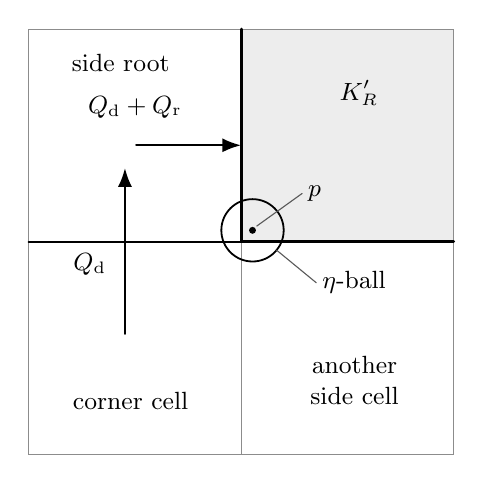
\begin{tikzpicture}[
  x=1.8cm,y=1.8cm,
  >=Latex,
  line cap=round,
  font=\small
]
  \fill[black!7] (0,0) rectangle (1.5,1.5);
  \draw[black!45,line width=.4pt] (-1.5,-1.5) rectangle (1.5,1.5);
  \draw[black!45,line width=.4pt] (0,-1.5) -- (0,0);
  \draw[line width=.65pt] (-1.5,0) -- (0,0);
  \draw[line width=1pt] (0,1.5) -- (0,0) -- (1.5,0);

  \node at (.83,1.05) {$K'_R$};
  \node at (-.85,1.26) {side root};
  \node at (-.78,-1.12) {corner cell};
  \node[align=center] at (.80,-.98) {another\\side cell};

  \draw[->,line width=.85pt] (-.82,-.65) -- (-.82,.52)
    node[pos=.42,left=3pt] {$Q_{\rm d}$};
  \draw[->,line width=.85pt] (-.74,.68) -- (0,.68);
  \node at (-.75,.95) {$Q_{\rm d}+Q_{\rm r}$};

  \draw[line width=.65pt] (.08,.08) circle[radius=.22];
  \fill (.08,.08) circle[radius=1.25pt];
  \draw[black!65,line width=.4pt] (.11,.11) -- (.43,.34);
  \node[anchor=west,inner sep=2pt] at (.43,.34) {$p$};
  \draw[black!65,line width=.4pt] (.25,-.06) -- (.53,-.29);
  \node[anchor=west,inner sep=2pt] at (.53,-.29) {$\eta$-ball};
\end{tikzpicture}
\caption{Auxiliary-cell routing near an inner corner (base-plane view).
The corner cell has no full face on $K'_R$, so its restricted
smeared mass $Q_{\rm d}$ is routed to the side root, whose own restricted
mass is $Q_{\rm r}$. The arrows indicate mass routing. On each outgoing
face, the assigned integrated outward flux is $-\kappa$ times the indicated
mass; the internal face fluxes cancel.
One retained center and the section of its $\eta$-ball are illustrated.
These auxiliary cells are independent of the large cells $H_i$ and of
the rectangles used for new particles. The completion field
$E_{\rm cross}$ is added to the other shell fields.}
\label{fig:normalized-corner-routing}
\end{figure}

The completion field is not cut at the boundaries of the large cells
$H_i$; thus no trace on an arbitrary such cut is required.
The local count estimate and bounded overlap of the unit trees give
\[
 \int w|E_{\rm cross}|^2
       \le C(1+g(\eta))\sum_{\rm trees}N_{\rm tree}^2,
 \qquad
 \int_{\partial K'_R\times\mathbb R^k}w j^2
       \le C\sum_{\rm trees}N_{\rm tree}^2
       \le C(1+M_{R,\eta'})\varepsilon^{-1}R.
\]
The additive $1$ in the count-square bound is required.

The crossing field now completes every retained smeared charge and provides
its actual outlet flux on the inner boundary. We next balance that flux
against the background, then choose an integer number of new particles.

For each large cell set
$Q_i=\int_{(\partial K'_R\cap\partial H_i)\times[-\ell,\ell]^k}w j$,
its actual inner-face outlet flux.  This need not equal the restricted
source mass $\kappa\rho_0(H_i\times[-\ell,\ell]^k)$, because the
completion field may transport that source across a large-cell boundary.
Define the ideal density by
\begin{equation}
 \kappa(m_i-1)|H_i|
       =B_i-\ell^\gamma(C^++C^-)|H_i|-Q_i.
 \label{eq:normalized-shell-density}
\end{equation}
Since $\sum_iQ_i=\kappa\rho_0(D_0^c)$, Gauss' equation and
\eqref{eq:normalized-two-caps} give
$\sum_i m_i|H_i|=R^2-N_{\rm old}=:N_{\rm new}\in\mathbb N$.
At fixed parameters the lateral-flux, cap-flux and outlet bounds make
$\max_i|m_i-1|\to0$ as $R\to\infty$; choose this maximum below $1/4$.
For example the outlet term divided by $|H_i|$ is bounded by
$C(1+M_{R,\eta'})\varepsilon^{-5}R^{-1}$.

Set $r_i=m_i|H_i|$.  Round the $r_i$ down, and increase the required
number of entries by one, obtaining integers $n_i$ with
$\sum_i n_i=N_{\rm new}$ and $|n_i-r_i|\le1$.
Put $\widetilde m_i=n_i/|H_i|$.  For large $R$ these densities lie
in $[1/2,3/2]$.  To compensate this rounding, write
$\delta_i=n_i-r_i$, whose sum is zero, and choose a rooted spanning
tree of the large-cell adjacency graph.  On the face from a child
cell $i$ to its parent prescribe outward weighted flux
$-\kappa\sum_{a\text{ in the subtree of }i}\delta_a$, with opposite
flux on the adjacent cell.  The total outward flux of cell $i$ is
$-\kappa\delta_i$.  There is therefore a compatible Neumann field
$E_{{\rm round},i}$ with source
$\kappa\delta_i|H_i|^{-1}\delta_{\mathbb R^2}$, these face fluxes,
and zero flux on all other faces, including the caps.
The paired fluxes make the union $E_{\rm round}$ a global field.
It has no flux through the inner or outer shell boundary.
After dilation by $\ell$, weighted trace and Poincar\'e on rectangles
of bounded aspect ratio give
\[
 \int w|E_{\rm round}|^2\le
 \begin{cases}C_{s,\varepsilon}\ell^{-s},&s>0,\\
 C_\varepsilon,&s=0.
 \end{cases}
\]
Indeed there are $O_\varepsilon(1)$ cells and each tree flux is
$O_\varepsilon(1)$; the unit-scale variational problem has bounded
energy, and dilation scales it by $\ell^{-s}$ for Riesz kernels and
by one for the logarithm.  This is $o(R^2)$ at fixed parameters.
For sufficiently large $R$, every sidelength of $H_i$ is at least
$\ell>2\sqrt2\ge2\widetilde m_i^{-1/2}$, and
$\widetilde m_i|H_i|=n_i\in\mathbb N$.
Thus Petrache and Serfaty~\citep[Lemma~6.3]{PetracheSerfaty2017} partitions $H_i$ into
$n_i$ rectangles of area $1/\widetilde m_i$, with every sidelength
in
\[
 \left[\frac14\widetilde m_i^{-1/2},
                      4\widetilde m_i^{-1/2}\right]
                  \subset[a_0,a_1].
\]
In particular, the lower bound $a_0$ fixed at the start applies to
every new-charge rectangle, independently of all later choices.

The vertical correction on each shell cell is the gradient of
\[
 h_2(y)=\frac{\ell^\gamma}{1-\gamma}
 \begin{cases}C^+y^{1-\gamma},&y\ge0,\\
 C^-|y|^{1-\gamma},&y\le0.
 \end{cases}
\]
It has source $-\ell^\gamma(C^++C^-)\delta_{\mathbb R^2}$.
The side-flux correction has the opposite cap source plus
$\kappa(m_i-1)\delta_{\mathbb R^2}$ and datum
$-E_\eta\cdot\nu_0+j$ on the
inner side, with zero data elsewhere.  Equation
\eqref{eq:normalized-shell-density} is exactly its compatibility.

The large-cell estimate used for this correction is as follows.
Let $H$ have sidelengths in $[\ell,2\ell]$, set
$\Omega=H\times[-\ell,\ell]$ and
$\Sigma=\partial H\times[-\ell,\ell]$, and let $-1<\gamma<1$.
For a constant $a$ and $b\in L^2(\Sigma,|y|^\gamma)$ satisfying
\[
              a|H|=-\int_\Sigma |y|^\gamma b,
\]
the weak Neumann problem
\[
 -\operatorname{div}(|y|^\gamma\nabla h)
                  =a\delta_{\mathbb R^2}\quad\hbox{in }\Omega,
 \qquad \partial_\nu h=b\quad\hbox{on }\Sigma,
 \qquad \partial_\nu h=0\quad\hbox{on }H\times\{\pm\ell\}
\]
has a solution modulo constants and obeys
\begin{equation}
 \int_\Omega |y|^\gamma|\nabla h|^2
 \le C_\gamma\left(a^2\ell^{3-\gamma}
              +\ell\int_\Sigma |y|^\gamma|b|^2\right)
 \le C_\gamma\ell\int_\Sigma |y|^\gamma|b|^2.
 \label{eq:large-cell-side-estimate}
\end{equation}
The constants depend only on $\gamma$ and the stated aspect-ratio
bounds.  To see the scaling, choose the weighted-mean-zero
representative.  Weighted Poincar\'e and the one-dimensional trace
inequalities, after dilation by $\ell$, give
\[
 \int_H|h(x,0)|^2\le C_\gamma\ell^{1-\gamma}
                              \int_\Omega |y|^\gamma|\nabla h|^2,
 \qquad
 \int_\Sigma |y|^\gamma|h|^2
          \le C_\gamma\ell\int_\Omega |y|^\gamma|\nabla h|^2.
\]
Testing the weak equation gives the first inequality in
\eqref{eq:large-cell-side-estimate}.
Compatibility, $|H|\asymp\ell^2$, and
$\int_\Sigma|y|^\gamma\asymp\ell^{\gamma+2}$ give
$a^2\ell^{3-\gamma}\le C_\gamma\ell\int_\Sigma|y|^\gamma|b|^2$,
which proves the second.  This is the constant-source case of
Petrache and Serfaty~\citep[Lemma~6.4]{PetracheSerfaty2017}, with the source coefficient
written explicitly.  For the logarithm use $\Omega=H$,
$-\Delta h=a$, and $\partial_\nu h=b$ on $\partial H$;
ordinary Poincar\'e, trace, and compatibility give the same final
bound $C\ell\int_{\partial H}|b|^2$.

For the side field on $H_i$, take
\[
 a_i=\kappa(m_i-1)+\ell^\gamma(C^++C^-),\qquad
 b_i=-E_\eta\cdot\nu_0+j
       \quad\hbox{on its inner face,}
\]
with $b_i=0$ on its other lateral faces.  The cap term is omitted
when $k=0$.  The density equation gives
$a_i|H_i|=B_i-Q_i=-\int_{\Sigma_i}w b_i$ exactly, so the cap
contribution to the constant source is included in the compatibility
estimate.  The inner faces partition the old lateral boundary.
Consequently the old-field coarea bound and the outlet bound yield
\begin{align*}
 \int w|E_{\rm side}|^2
 &\le C_s\ell\sum_i\int_{\Sigma_i}w|b_i|^2\\
 &\le C_s\ell\left(
      \int_{\partial K'_R\times[-\ell,\ell]^k}w|E_\eta|^2
          +\int_{\partial K'_R\times\mathbb R^k}wj^2\right)\\
 &\le C_{s,\eta'}(\varepsilon^2R)(\varepsilon^{-1}R)
                    (M_{R,\eta}+1+M_{R,\eta'})\\
 &=C_{s,\eta'}\varepsilon R^2(M_{R,\eta}+1+M_{R,\eta'}).
\end{align*}
Here $\Sigma_i=\partial H_i\times[-\ell,\ell]^k$.
This calculation supplies the length factor in the side-field row
of the shell-energy estimate.  Its constant may depend on the single
fixed auxiliary cutoff $\eta'$, but not on $\eta$, $\varepsilon$,
$R$, or the realization.

Finally, let $S\subset H_i$ be one of the area-$1/\widetilde m_i$
rectangles, with barycenter $p$, and work on the fixed cylinder
$\Omega_S=S\times(-1,1)^k$ (or $\Omega_S=S$ when $k=0$).
Take the $\eta$-truncation of the neutral Neumann field with source
$\kappa(\delta_{(p,0)}-\widetilde m_i\mathbf1_S\delta_{\mathbb R^2})$
and zero normal component on its entire boundary.  The truncated source is
$\kappa(\delta_p^{(\eta)}-\widetilde m_i\mathbf1_S\delta_{\mathbb R^2})$.
Extend this truncated field by zero into $H_i\times[-\ell,\ell]^k$
and the shell.  The sidelength bounds $[a_0,a_1]$, fixed height, and
$\eta<a_0/16$ keep the charge uniformly away from the cell boundary.
To verify its energy, write the point-source potential as
$g(\cdot-(p,0))+v$. The correction solves
\[
 Lv=-\kappa\widetilde m_i\mathbf1_S\delta_{\R^2},\qquad
 \partial_\nu v=-\partial_\nu g(\cdot-(p,0))
                       \quad\hbox{on }\partial\Omega_S.
\]
The weighted trace and Poincar\'e estimates give a uniform bound on
$\int_{\Omega_S}w|\nabla v|^2$; no smoothness across $y=0$ is needed.
Test this compatible weak equation against $g_\eta(\cdot-(p,0))$.
The resulting plane integral is uniformly bounded because $s<2$, and
the boundary terms are uniformly bounded by the clearance from the pole.
Hence $\int_{\Omega_S}w\nabla v\cdot\nabla g_\eta=O_s(1)$.
The capped fundamental solution itself has energy
$\kappa g(\eta)+O_s(1)$ in $\Omega_S$, so the truncated cell field has
the same energy, uniformly over the allowed rectangles.
In addition to the preceding $o(R^2)$ bound for $E_{\rm round}$,
the shell fields satisfy
\begin{align*}
 \int w|E_{\rm cross}|^2
   &\le C(1+g(\eta))(1+M_{R,\eta'})\varepsilon^{-1}R,\\
 \int w|E_{\rm vert}|^2
   &\le C e_{\varepsilon,R}\varepsilon^3R^2,\\
 \int w|E_{\rm side}|^2
   &\le C_{s,\eta'}\varepsilon(M_{R,\eta}+1+M_{R,\eta'})R^2,\\
 \int w|E_{\rm new}|^2
   &\le C(1+g(\eta))N_{\rm new},
\end{align*}
where $N_{\rm new}=O(\varepsilon R^2)+o(R^2)$ at fixed parameters.
The first bound uses the sum of squared tree counts; the third
uses the weighted rectangle trace estimate with height $\ell$.
Write $\nu_{{\rm new},\eta}=\sum_{p\ {\rm new}}\delta_p^{(\eta)}$.
The five shell fields have combined source
\[
 \kappa\rho_0
 -\ell^\gamma(C^++C^-)\delta_{\mathbb R^2}
 +\bigl[\kappa(m_i-1)+\ell^\gamma(C^++C^-)\bigr]\delta_{\mathbb R^2}
 +\kappa(\widetilde m_i-m_i)\delta_{\mathbb R^2}
 +\kappa(\nu_{{\rm new},\eta}-\widetilde m_i\delta_{\mathbb R^2}),
\]
which is $\kappa(\rho_0+\nu_{{\rm new},\eta}-\delta_{\mathbb R^2})$.
On the inner shell boundary the crossing and side data sum to
$-j+(-E_\eta\cdot\nu_0+j)=-E_\eta\cdot\nu_0$.
The rounding field has zero inner data and paired internal data;
the completion field remains global across the large-cell boundaries.
Thus all interface fluxes cancel.  We sum squared energies only in
the shell, where a fixed factor of five is harmless.  The old field
inside $D_0$ is retained exactly, with coefficient one in the energy
bound; no global factor multiplying its energy is introduced.

The shell now has the required source and lateral flux. It remains to close
the two vertical ends without changing these sources.

The upper and lower weighted harmonic caps are solved separately.
On the inner horizontal face of the upper or lower cap, prescribe the
outward normal derivative $-E_\eta(x,\pm\ell)\cdot(\pm e_y)$ for
$x\in K'_R$, and $-C^\pm$ for $x\in K_R\setminus K'_R$; here $e_y$
is the positive vertical unit vector.  Prescribe zero normal derivative
on every other face.  By \eqref{eq:normalized-two-caps}, the weighted
integral of these data is
$-T_\pm-A_{\rm sh}\ell^\gamma C^\pm=0$, so each cap problem is
compatible.  If $u$ is adjusted by its ordinary mean on one cap,
ordinary trace and Poincar\'e, followed by weight comparison, give
\[
 \int_{K_R\times\{\ell\}}w|u|^2
   \le CR\max\{1,(\ell/R)^\gamma\}
                              \int_{\rm cap}w|\nabla u|^2.
\]
Testing the compatible cap problem yields total cap energy at most
\[
       C e_{\varepsilon,R}
                     \varepsilon^{1+\min(2\gamma,0)}R^2.
\]
The extra factor for $\gamma<0$ is retained.  It vanishes at fixed
$\varepsilon$ by \eqref{eq:normalized-moving-tail}.
There are no cap terms for $k=0$.

Retain $E_\eta$ in $D_0$, use the sum of the five finite-energy
components in the shell, and use the two harmonic cap fields above
and below.  Extend this assembled field $\widehat F_\eta$ by zero past the
outer square and the cap heights.  It has zero exterior normal flux
and source $\kappa(\sum_{p\in\widehat\Lambda}\delta_p^{(\eta)}
-\mathbf1_{K_R}\delta_{\mathbb R^2})$, where
$\widehat\Lambda$ consists of the retained old and new barycenter
charges, exactly $R^2$ points.  Now define
\[
 \widehat E=\widehat F_\eta+
               \sum_{p\in\widehat\Lambda}\nabla f_\eta(\cdot-(p,0)).
\]
The singular corrections lie inside the outer square by its clearance.
Thus $\widehat E_\eta=\widehat F_\eta$ exactly, and the fundamental-solution
identity proves the required unsmeared divergence equation, with
zero exterior normal flux.  At fixed cutoffs the preceding bounds
give
\begin{align}
 R^{-2}\int_{K_R\times\mathbb R^k}w|\widehat E_\eta|^2
 &\le M_{R,\eta}
   +C_{s,\eta'}\varepsilon(1+g(\eta))
                 (1+M_{R,\eta}+M_{R,\eta'})+o_R(1)\notag\\
 &\quad+C_s e_{\varepsilon,R}
                       \varepsilon^{1+\min(2\gamma,0)}.
 \label{eq:normalized-screen-estimate}
\end{align}
Here $R$ is chosen after $\eta,\eta',\varepsilon$.
For example, the count estimate is controlled once $R\gg(1+M_{R,\eta'})\varepsilon^{-5}$.

Every new barycenter is at least $a_0/2$ from each face of its
rectangle.  Retained old points lie inside $K'_R$ or within $\eta$
of its boundary.  Since $\eta<\eta_0\le a_0/16$ was fixed before
the realization was selected, every new--old distance is at least
$a_0/2-\eta>2\eta$.
Choose the integer radius large enough that
$\varepsilon R-\eta\ge a_0/2$; this gives the same clearance at
the outer boundary and hence at every reflected seam.
New--new distances and all reflection-seam distances exceed $2\eta$.
Thus every close pair after screening was already an old close pair.

\end{proof}

\subsection{Reflection, projection, and removal of the cutoff}

\begin{proof}[Proof of Proposition~\ref{prop:normalized-cubic-approximation}]
Lemma~\ref{lem:field-cutoff-control} proves existence and the uniform lower
bound of the cutoff limit, as well as finiteness of $m$. To approximate $m$,
choose a selected dyadic cutoff $\eta$ and a realization supplied by
Lemma~\ref{lem:stationary-field-minimizers}. Apply
Lemma~\ref{lem:field-screening} after choosing $\varepsilon$, and then
choose its integer radius $R$. We now convert that screened field into a
canonical periodic gradient and estimate its energy after removing the
cutoff.

Reflect the screened square in both coordinate directions and repeat
with period $2R\mathbb Z^2$.  The reflected vector components have
matching zero normal flux, so there are no interface charges.  The
period cell has $4R^2$ points and area $4R^2$.
Reflection multiplies both energy and defect by four.  The nonnegative
defect of the resulting configuration is at most the old anchored
defect in $K_R$, divided by $R^2$, and hence tends to at most
$d_\eta(E)\le2D_\eta$.

Write $E^{\rm per}$ for the reflected field, which need not be curl free,
and let $E^{\rm can}$ be the canonical periodic gradient with exactly
its charges and background. At fixed cutoff,
$D=E^{\rm per}-E^{\rm can}=E^{\rm per}_\eta-E^{\rm can}_\eta$
belongs to $L^2(w)$ on the full period cylinder and has zero weighted
divergence.  Test against the canonical truncated potential, with
vertical cutoffs tending to infinity; its nonconstant Fourier modes
decay vertically and its zero mode has compactly supported derivative.
The cross term vanishes, so
\[
 \int_{T\times\mathbb R^k}w|E^{\rm per}_\eta|^2
  =\int_{T\times\mathbb R^k}w|E^{\rm can}_\eta|^2
                       +\int_{T\times\mathbb R^k}w|D|^2.
\]
Canonical projection therefore decreases the cutoff energy and leaves
the configuration defect unchanged. It also returns to the prescribed
admissible class. For $s>0$, finite truncated $L^2(w)$ energy gives local
unweighted $L^p$ by weighted H\"older when $p<\min(2,2/s)$, and each of
the finitely many local singular corrections belongs to $L^p$ when
$p<3/(s+1)$.
For the logarithm both bounds reduce to $p<2$. Weighted Cauchy--Schwarz
and the locally integrable singular flux give $wE^{\rm can}\in
L^1_{\rm loc}$. Thus the canonical gradient is a member of
$\mathcal A_1$ with the exponent fixed at the beginning, even though the
intermediate screened field was not required to be a gradient.

For a finite simple periodic configuration, integrate
\eqref{eq:normalized-two-cutoff-local} over its period cell and let the
auxiliary cutoff tend to zero. This gives
\begin{equation}
 V(\mathcal C)-\mathcal W_\eta(E^{\rm can}_{\mathcal C})
   =\frac{\kappa}{|T|}\sum_{p\in T}\sum_{q\ne p}q_\eta(p-q)
                        -2\kappa F_\eta.
 \label{eq:normalized-periodic-defect}
\end{equation}
The second sum includes periodic images; the self image at zero is
the only omitted particle.

Keep the auxiliary cutoff $\eta'$ fixed at its initial value as $\eta$
tends to zero.  For each selected $\eta$, take the realization chosen
above, and choose $\varepsilon$ so the middle
term of \eqref{eq:normalized-screen-estimate} is as small as desired;
then choose an arbitrarily large integer $R$ so that all energy and
defect limits, the moving-tail estimate, the size conditions, and the
seam clearance hold simultaneously.  Subtract $\kappa g(\eta)$,
project canonically, and apply \eqref{eq:normalized-periodic-defect}.
Equations \eqref{eq:normalized-cutoff-bound} and
\eqref{eq:normalized-defect-small} give
\[
 V(\mathcal C_{\eta,R})
   \le m+2\kappa F_\eta+o(1)+2D_\eta-2\kappa F_\eta
   =m+2D_\eta+o(1).
\]
Let the chosen cutoffs tend to zero, taking the screening thickness
and integer radius in that order for each cutoff.  The canonical
periodic gradients belong to $\mathcal A_1$, so their values are also
at least $m$.  This proves the asserted cubic minimizing sequence.
Every use of the box limit preceded removal of the cutoff; no
interchange of the two limits has been made.
\end{proof}

\section{An alternative rational verification procedure}
\label{app:floor-certificate}

This appendix proves a conditional alternative to the exact-array interval
verification used in Proposition~\ref{prop:finite-certificate}.  If the
rational procedure below passes the stronger tables of
Section~\ref{sec:finite}, its roundoff allowances leave the exact quadrature
arrays within the proposition's looser bounds.  The complete floor-rounded
matrix procedure is not executed by the supplied programs; the selected
finite certificate uses direct Arb enclosures of the exact arrays.

We use $\epsilon=10^{-80}$ and the decimal brackets $p_*,b_*$ from
\eqref{eq:rational-pi-b} in Appendix~\ref{sec:arithmetic}.  We first define
the rounding and prove its error bounds.  The complete listings then specify
each finite loop, keeping all arithmetic not explicitly rounded exact.

\subsection{Componentwise rounding and its error}

For real $x$, let $R(x)=\epsilon\lfloor x/\epsilon\rfloor$.  Apply $R$
separately to the real and imaginary components of a complex number and
entrywise to a matrix.  For complex rational $w$, define
\begin{equation}\label{eq:rational-exponential}
\begin{gathered}
 u=R(w/4096),\qquad d_0=1,\qquad
 d_j=R(d_{j-1}u/j)\quad(1\le j\le60),\\
 x_0=\sum_{j=0}^{60}d_j,\qquad
 x_{j+1}=R(x_j^2)\quad(0\le j<12),\qquad e_*(w)=x_{12}.
\end{gathered}
\end{equation}
This uses a degree-$60$ polynomial with $61$ terms followed by twelve
squarings.  Every quantity is rational.  In the floor prescription,
$\pi,b,\sqrt3$ are replaced by $p_*,b_*,2b_*$, cosine is evaluated as
$\Rea e_*(iw)$ at the corresponding rational phase $w$, and $B,h$ remain
exact.

In addition to the floors internal to $e_*$, the prescription rounds the
quadrature points and weights, mass entries, and values of $z$ and $\lambda$.
It rounds the transformed zeroth moment factor and every higher moment
factor after its divided-power update.  It also rounds the projected jet
entries, the entries of $Y$, every product in the power and partial-sum
updates, and both final positive-node coefficient matrices.  The extra
coordinates and all other operations are exact rational arithmetic; in
particular, the products used to form the Bernstein and tail rows incur no
further floors.  The listings below fix the order of these operations.

A superscript $\#$ denotes the output of this floor prescription.  Its
error is measured against the corresponding exact quadrature array of
Section~\ref{sec:finite}: for example,
$S^\#_{\mathcal F\mathcal F}$ is compared with
$\widetilde S_{\mathcal F\mathcal F}$, $S^\#_{\mathcal F e}$ with
$\widetilde S_{\mathcal F e}$, and $Y^\#,X_i^\#$ with $Y,X_i$.
The error from quadrature to the exact spectral integrals is a different
quantity, already bounded in Lemma~\ref{lem:quadrature-error}.

\Needspace{6\baselineskip}
\begin{lemma}[Roundoff bounds for rational verification]
\label{lem:rational-roundoff}
The floor prescription below has the following properties.
\begin{enumerate}
\item If $|w|<1700$ and $\Rea w<7$, then $|e_*(w)-e^w|<10^{-68}$.
Every exponential argument in the prescription lies in this domain.
\item A computed single-column quadrature moment of order at most $42$,
scaled by $y^a/a!$ with $|y|\le3/2$, differs from the exact quadrature
moment by less than $10^{-48}$.  The initial operator-norm errors in
$S^\#_{\mathcal F\mathcal F}$, $S^\#_{\mathcal F e}$, and $Y^\#$ are
less than $10^{-44}$.
\item Suppose that either the exact or the rounded computation satisfies
the following envelopes: every pre-update power in the nine steps has norm
below $3$, each intermediate partial-sum matrix has norm below $34$, and
every combined pair of corresponding $X_1,X_2$ columns has norm below $5.6$.
Then the combined error in a pair of corresponding columns of
$X_1^\#,X_2^\#$ is less than $10^{-29}$.
Every entry of the Bernstein rows $L_{i,d}^\#$ differs from the
corresponding entry of $L_{i,d}$ in \eqref{eq:bernstein-rows} by less than
$10^{-16}$.  Every lower evaluation in \eqref{eq:bernstein-certificate}
and every tail expression in \eqref{eq:tail-certificate} has error less
than $10^{-6}$.
\end{enumerate}
The stagewise envelopes in the last item follow from the stronger power and
column tables, whether those tests are established on the exact arrays by
intervals or on the rounded arrays by the prescription below.
\end{lemma}

\begin{proof}
We control elementary functions first, then a single moment, then the
matrix products, and finally the scalar lower evaluations.  This order
keeps the error due to the coefficient lists separate from the error in
the primitive moments.

\paragraph{Exponential approximation.}
A componentwise floor changes a complex number by less than $2\epsilon$.
For $r=w/4096$, both $|r|$ and $|u|$ are below $.416$.  If $\delta_j$
bounds $|d_j-r^j/j!|$, then
\[
 \delta_0=0,\qquad
 \delta_j\le\frac{.416}{j}\delta_{j-1}
 +\frac{2\epsilon\,.416^{j-1}}{j!}+2\epsilon.
\]
The first term propagates the previous error, the second changes $r$ to
$u$, and the last is the new floor.  Summing through $j=60$ and adding
the exponential tail gives
\[
 |x_0-e^{w/4096}|
 \le\sum_{j=0}^{60}\delta_j+\frac{e^{.416}.416^{61}}{61!}
 <1.263\cdot10^{-78}<4\cdot10^{-78}.
\]
The factorial tail alone is less than $4\cdot10^{-107}$.  These are finite
rational comparisons after using $e^{.416}<e<2719/1000$.

At squaring step $j$, the exact value has modulus at most
$e^{7/2^{12-j}}$.  While the accumulated error is below one, its
amplification factor is at most $2e^{7/2^{12-j}}+1$.
Since $2e^a+1\le3e^a$ for $a\ge0$, the product of all twelve factors
is at most $3^{12}e^7$.  Including all twelve new floors gives
\begin{equation}\label{eq:exponential-roundoff-budget}
 (4\cdot10^{-78}+24\epsilon)3^{12}e^7
 <2.472\cdot10^{-69}<10^{-68}.
\end{equation}
The same bound is below one at every earlier stage, closing the hypothesis
used in the amplification estimate.

The arguments used by the prescription have ample room in the stated domain.
Density phases have modulus at most $\pi\cdot168$ before the rational
perturbations.  The weight cosines have phase modulus less than
$2\pi\cdot191$.  Transformed phases have modulus at most
$\pi(44/15)168<1549$ and nonpositive real part by
Lemma~\ref{lem:kernel-bounds}.  They remain in the left half-plane after
substitution: on the real integration interval, $\Ima z>.187/\pi$,
whereas the perturbation of $z$ below is less than $10^{-65}$.
The only positive real scalar phases are $K\le6$ in the support at $m=0$.
Every other finite scalar phase is nonpositive with modulus at most $48$.
Infinite endpoints are evaluated by their limits, not passed to $e_*$.
Thus every call satisfies $|w|<1700$ and $\Rea w<7$.

\paragraph{Primitive masses and moments.}
The intermediate absolute error allowances are
\begin{equation}\label{eq:primitive-roundoff-budgets}
\begin{array}{c|c}
\text{quantity}&\text{absolute error bound}\\ \hline
 \tau_{jv}&10^{-67}\\
 o_v&10^{-65}/384\\
 z(t),\ \lambda(t)&10^{-65}\\
 \text{one density value}&10^{-60}\\
 \text{one mass column, summed absolute error}&10^{-59}\\
 F_0(t),\ G_0(t)&10^{-60}\\
 F_a(t),\ G_a(t),\quad0\le a\le42&10^{-52}\\
 Q_n,\ D_n&10^{-75}.
\end{array}
\end{equation}
The comparison values here use the exact quadrature points and the exact
constants $\pi,b$.  We justify each stage rather than infer it from decimal
agreement.

For a weight phase, replacing $\pi$ changes the phase by less than
$382\epsilon$.  Add the $10^{-68}$ exponential error, and use
$2\sum_{a=1}^{191}(4a^2-1)^{-1}<1$.  Including the final floor gives
the stated bounds for $\tau$ and $o$.  On the real line, $|t+ih|\ge h$;
the derivative bounds
\[
 |z'(t)|\le B/h^2<9,\qquad
 |\partial_t\lambda(t)|<8,\qquad |\partial_b\lambda(t)|<4
\]
then give the errors for $z$ and $\lambda$.  The density phase errors
are below $10^{-63}$ because $n\le168$.  Inserting them in the six-term
density formulas, using $\sum_{l>0}|P_l|=10$, gives the density allowance
$10^{-60}$. The weighted density errors sum to at most $10^{-60}$ because
the six positive quadrature rules have total weight one. Weight errors,
density errors, the $2311$ componentwise mass floors, and atom coefficient
errors together contribute less than $10^{-59}$
to the sum of absolute errors in one mass column.

Each exact mass column has sum of absolute values less than $230$.  Indeed,
the pointwise real-interval density bounds are
$2\pi^2\sum_{l>0}t_l|P_l|<106$ for a $c_n$ column and $20\pi<63$ for a
$d_n$ column; the constant column has atomic variation $25$.  Positivity
and total density weight one from \eqref{eq:positive-quadrature-weights}
make $230$ a common bound.

The direct zeroth kernel phase error is below $10^{-63}$.  The transformed
zeroth phase error is below $6\cdot10^{-63}$, and multiplication by
$|\lambda|<3$ still leaves error below $10^{-60}$.  The divided-power
arguments $i\pi yt$ and $i\pi yz$ have modulus below $15$ and error below
$10^{-63}$.  To see explicitly how these errors enter a higher moment, write
either exact factor as $H_a=H_0v^a/a!$ and its rounded update as
$H_a^\#=R(H_{a-1}^\#v^\#/a)$.  Here
\[
 |H_0|<3,\qquad |H_0^\#-H_0|<10^{-60},\qquad
 |v|,|v^\#|<15,\qquad |v^\#-v|<10^{-63}.
\]
Changing the initial value costs at most $e^{15}10^{-60}$, and changing
$v$ costs at most $3e^{15}10^{-63}$, by the derivative of $v^a/a!$.
A floor introduced at step $j$ is multiplied by
$(v^\#)^{a-j}j!/a!$.  Since $j!/a!\le1/(a-j)!$, all the floors together
cost at most
\[
 2\epsilon\sum_{j=1}^a15^{a-j}\frac{j!}{a!}\le2\epsilon e^{15}.
\]
Thus for $0\le a\le42$ the total factor error is bounded by
\[
 |H_a^\#-H_a|
 <e^{15}\bigl(10^{-60}+3\cdot10^{-63}+2\epsilon\bigr)<10^{-52}.
\]
The last comparison follows already from $e<3$.
Expanding the moment difference against the rounded mass column, whose norm
is below $230+10^{-59}$,
also retains the product of the two primitive errors.  The total is at most
\[
 (230+10^{-59})10^{-52}+3e^{15}\cdot10^{-59}<10^{-48}.
\]
Finally, \eqref{eq:node-constants} and \eqref{eq:rational-pi-b-error}
give errors below $10^{-75}$ in $Q_n,D_n$.  Jet projection uses
$Q_n>1.75$, $|D_n|<2.12$, and $168$ output coordinates.  Including its
floors, the resulting initial operator errors are less than $10^{-44}$;
the same estimate applies to $Y^\#$.

\paragraph{Powers and coefficient columns.}
A floor on a real matrix with $168$ rows contributes at most
$168\epsilon<10^{-77}$ in operator norm.  Let $e_r$ bound the error in
$U$ before step $r$, and let $v_r$ bound the error in either partial-sum
matrix after $r$ steps, with $v_0=0$.  The assumed stagewise envelopes give
$\norm{U}<3$ and partial-sum norms below $34$.  Comparing products and
then adding the floor gives
\begin{equation}\label{eq:matrix-roundoff-recurrence}
 e_0<10^{-44},\qquad
 e_{r+1}\le7e_r+10^{-77},\qquad
 v_{r+1}\le5v_r+34e_r+10^{-77}.
\end{equation}
More precisely, the square error is at most $(6+e_r)e_r+10^{-77}$,
and the partial-sum coefficient of $v_r$ is at most $4+e_r$.
Induction gives $e_r<1$ and validates the displayed recurrence.  Its
finite rational solution yields
\[
 \max_{0\le r\le8}e_r<5.765\cdot10^{-38}<10^{-36},
 \qquad v_9<6.529\cdot10^{-36}<10^{-34}.
\]
If the coarse norms are known for the rounded rather than exact factors,
exchange their roles in the product difference.  The same two inequalities
follow.  This is why the argument is not circular and does not require a
rounded matrix inverse.

The largest combined column norm of $E_1,E_2$ is $3.3505$.
The formulas for $Y$ give $\norm{Y}<2$, and the transform bound gives
the sharper data estimate
$2+(4000+2\cdot10^{-27})3.3505<13405$.
Its rational perturbation is less than $10^{-43}$. Thus, for every column $j$,
$\norm{(g_1)_j}_1+\norm{(g_2)_j}_1<20000$ for both the exact and rounded data.
Applying the two sum/difference formulas in
\eqref{eq:finite-columns}, including the $168$ real floors in each of
the two final columns, gives the complete bound
\[
 40000v_9+72\cdot10^{-43}+336\epsilon
 <2.612\cdot10^{-31}<10^{-29}.
\]
The appended extras are exact.  In particular, the term $336\epsilon$ is
part of the column error even though it is negligible numerically.

\paragraph{Bernstein and lower-evaluation errors.}
A scaled moment against a unit list column has absolute value at most
$230\cdot3e^{15}$.  Also $|y|^{-\nu}\le4$ and
$0\le\omega_{dr}\le1$.  The contribution from the coefficient-list error
to one Bernstein row entry is therefore at most
\[
 41\cdot4\cdot230\cdot3e^{15}\cdot10^{-29}
 <3.700\cdot10^{-18}.
\]
For this decomposition the list difference is evaluated with exact moments;
the primitive difference is evaluated against the rounded columns.
The primitive moments therefore contribute separately.  The relevant combined
column norm is below $6$, either directly from the rounded cutoffs or
from the exact cutoff $5.6$ and the column error.  Thus their contribution
is at most
\[
 41\cdot4\cdot6\cdot10^{-48}<10^{-44}.
\]
The sum of these two contributions is below $10^{-16}$, as claimed.
This explicitly includes the primitive-moment addition.

For completeness, the subsequent minimizations do not amplify that bound
to anything close to $10^{-6}$.  The same moment bound with combined
column norm $6$ shows that each exact Bernstein row entry is below $10^{14}$
in modulus.  If its entry error is $\delta=10^{-16}$, then for
$x\in\{1/K,1/J\}\subset[0,1]$ the error in $a_j+xb_j$ is below $2\delta$.
A finite endpoint exponential has error below $10^{-68}$ and modulus at
most one; the infinite-endpoint values are exact.  Each product in
\eqref{eq:box-lower} consequently has error below
$2\delta+(2\cdot10^{14}+2\delta)10^{-68}$.  There are four such products
and one unmultiplied term.  A minimum is nonexpansive in the maximum norm,
so the total row lower-evaluation error is less than $2\cdot10^{-15}$.

Only the target supports at $m=0$ and $m=3$ use a rounded exponential.
At $m=0$, $|Ky|\le3$, $1/K<1$, and
$\sum_{r=0}^{40}3^r/r!<e^3<27$, so their total weighted error is below
$27\cdot10^{-68}$.  At $m=3$, $J/2\le3$ gives error below
$3\cdot10^{-68}$.  The $m=1$ support is rational and exact.  These
additions still leave a bound far below $10^{-6}$.

For a tail row from $X_i$, the entry error is below $10^{-29}$ and its
entry modulus is below $6$.  The same is true for the row obtained by
summing the low $d_n$ rows, because the combined column norm controls that
sum.  The preceding five-term argument gives lower-evaluation error below
$2\cdot10^{-28}$ for each such row.  Taking $\min(0,\cdot)$ does not
increase it.  In \eqref{eq:tail-certificate} there are one constant row,
one summed row, and two rows for each of $46$ low nodes, hence $94$ terms.
Their nonnegative reciprocal factors are at most one since $s_0-n\ge1.5$.
The tail error is therefore below $94(2\cdot10^{-28})<2\cdot10^{-26}$,
in particular below $10^{-6}$.
\end{proof}

\subsection{The complete floor-rounded finite prescription}

We now specify the alternative rational computation.  Every loop has a
finite inclusive range.  The five shell and two list indices are one-based;
quadrature and derivative indices start at zero as indicated.  Products
are ordinary matrix or row products, without conjugation.  An operation
not marked $R$ is exact rational arithmetic.  The imaginary unit is
\texttt{i}; a list subscript never denotes that unit.  The symbols
$P_l,Q_n,D_n$ mean the formulas in \eqref{eq:periodic-coefficients} and
\eqref{eq:node-constants} after the rational substitutions above.

The input order is all $c_n$ for increasing $n\in\mathcal F$, then all
$d_n$, then $c_0,d_0,C$.  The $2311$ mass rows are the $6\cdot384$
quadrature points in lexicographic order followed by the seven atoms.

\Needspace{12\baselineskip}
\begin{lstlisting}[basicstyle=\ttfamily\footnotesize,columns=fullflexible,
breaklines=true,frame=single,caption={Floor-rounded verification: masses and moment factors},label=alg:finite-verification]
eps = 1/10^80
R(x) = eps * floor(x/eps)  # separately on complex components
# pstar,bStar are the two printed 80-digit decimal rationals.
# e_star uses the degree-60 Taylor polynomial and 12 squarings above.

F_nodes = [n for n=1..168 if n mod 12 in {0,1,3,4,7,9}]
t_l = l/6 for l=0..6
for v=0..383:
    a0 = (v+1/2)/384
    o[v] = R((1-2*sum(Re(e_star(2*d*i*pstar*a0))/(4*d*d-1)
                          for d=1..191))/384)
    for j=1..6:
        tau[j,v] = R((2*j-1+Re(e_star(i*pstar*a0)))/12)

W = zero complex matrix with 2311 rows and 171 columns
for j=1..6:
  for v=0..383:
    t = tau[j,v]
    for n in F_nodes followed by [0]:
      for l=j..6:
        A[l] = (o[v]/6)*2*pstar*e_star(-i*pstar*t*n)
                            *P[l]*e_star(i*pstar*t_l*n)
      W[(j,v),c(n)] = R(-pstar*sum((t_l-t)*A[l] for l=j..6))
      W[(j,v),d(n)] = R(i*sum(A[l] for l=j..6))
for j=0..6:
    W[atom(j),C] = R((1 if j==0 else 2)*P[j])

function factors(m,y,end_degree):
    points = all tau[j,v], followed by t_0,...,t_6
    for each point t:
        z[t] = R(-B/(t+i*h)-i*h)
        lam[t] = R(i/(bStar*(t+i*h)))
        F[0,t] = e_star(i*pstar*t*m)
        G[0,t] = R(lam[t]*e_star(i*pstar*z[t]*m))
        for a=1..end_degree:
            F[a,t] = R(F[a-1,t]*i*pstar*t*y/a)
            G[a,t] = R(G[a-1,t]*i*pstar*z[t]*y/a)
    return F,G
\end{lstlisting}

These moments are scaled by $y^a/a!$, which explains the division by
$y^\nu$ in the later half-gap rows.  The floor convention can itself be
implemented with integers.  Put $S=10^{80}$.  For $w=w_r+iw_i$, initialize
$u_r=\lfloor Sw_r/4096\rfloor$ and
$u_i=\lfloor Sw_i/4096\rfloor$.  Represent a rounded complex number by
the two integers obtained after multiplication by $S$.  The Taylor update is
\[
 (d_r,d_i)\longmapsto
 \left(
 \left\lfloor\frac{d_ru_r-d_iu_i}{Sj}\right\rfloor,
 \left\lfloor\frac{d_ru_i+d_iu_r}{Sj}\right\rfloor
 \right),
\]
with both right sides evaluated before replacement.  The squaring update is
\[
 (x_r,x_i)\longmapsto
 \left(
 \left\lfloor\frac{x_r^2-x_i^2}{S}\right\rfloor,
 \left\lfloor\frac{2x_rx_i}{S}\right\rfloor
 \right).
\]
Every floor is toward negative infinity, including for negative numerators.
These formulas are exactly \eqref{eq:rational-exponential}.

\Needspace{12\baselineskip}
\begin{lstlisting}[basicstyle=\ttfamily\footnotesize,columns=fullflexible,
breaklines=true,frame=single,caption={Floor-rounded verification: projected matrices and columns},label=alg:finite-columns]
Ssharp = zero matrix with 168 rows and 171 columns
Ysharp = zero matrix with 168 rows and 10 columns
for m in F_nodes:
    F,G = factors(m,1,1)
    a = Re(G[0,:] * W)
    d = Re(G[1,:] * W)
    Ssharp[c(m),:] = R(-a/Q_m)
    Ssharp[d(m),:] = R((D_m*a-d)/Q_m)
for j=1..5:
    n = [1,3,4,7,9][j]
    Ysharp[d(n),j]   = R(-1/Q_n)
    Ysharp[c(n),j+5] = R(1/Q_n)
    Ysharp[d(n),j+5] = R(-D_n/Q_n)

E = zero matrix with 6 rows and 10 columns
E[:,1] = [.567,.250,-.0074,0,-.209,.0096]
E[:,6] = [-.976,.408,.0115,1,.938,-.017]
E1 = first three rows of E
E2 = last three rows of E
U = positive-coordinate columns of Ssharp
vp = identity matrix of size 168
vm = identity matrix of size 168
for r=0..8:
    vp = vp + R(vp*U)
    vm = vm + R((-1 if r==0 else 1)*vm*U)
    record the maximum absolute column sums of U,vp,vm
    if r<8: U = R(U*U)
# Compare every recorded value with the power table, row r.

Se = last three columns of Ssharp
g1 = Ysharp + Se*E2
g2 = Se*E1
X[1] = stack(R((vp*(g1+g2)+vm*(g1-g2))/2), E1)
X[2] = stack(R((vp*(g1+g2)-vm*(g1-g2))/2), E2)
# Test every individual and same-column combined absolute column sum
# against the corresponding bound in the column table.
\end{lstlisting}

The product identities in the proof of
Proposition~\ref{prop:finite-certificate} give the prescribed $512$-term
series.  At each stage, the entries of \texttt{vp} and \texttt{vm} are
integer multiples of $\epsilon$.  Hence
$V+R(VU)=R(V(I+U))$, with the analogous identity for the initial minus
sign.  The listing and the rounded product update used in
\eqref{eq:matrix-roundoff-recurrence} are therefore the same operation.

\Needspace{12\baselineskip}
\begin{lstlisting}[basicstyle=\ttfamily\footnotesize,columns=fullflexible,
breaklines=true,frame=single,caption={Floor-rounded verification: every half-gap and tail inequality},label=alg:finite-signs]
nodes5 = [1,3,4,7,9]
endpoints = [2.36,2.65,3.2,4,6,infinity]
sigma = [-1,1]

function low(row,K,J):
    exK = [e_star(-K*(n-1)) for n in nodes5]
    exJ = ([e_star(-J*(n-1)) for n in nodes5]
                   if J<infinity else [1,0,0,0,0])
    answers = []
    for x in [1/K, (1/J if J<infinity else 0)]:
        v = row[1..5] + x*row[6..10]
        answers.append(v[1] + sum(min(v[a]*exK[a],v[a]*exJ[a])
                                                     for a=2..5))
    return min(answers)

low_nodes = [0] followed by all n in F_nodes with n<=88
for m in low_nodes:
    # Successor and predecessor are in {0} union the positive nodes.
    ys = [(successor(m)-m)/2]
    if m>0: append (predecessor(m)-m)/2 to ys
    for y in ys:
        nu = (0 if m==0 else 2)
        F,G = factors(m,y,40+nu)
        for fn=1..2:
            for a=0..40:
                l[a] = sigma[fn]/y^nu * Re(
                    F[a+nu,:]*(W*X[fn])
                    +G[a+nu,:]*(W*X[3-fn]))
            for consecutive K,J in endpoints:
                tc = zero row of length 41
                if m==0:
                    tc[r] = e_star(K)/K * (-K*y)^r/r! for r=0..40
                if m==1:
                    tc[r] = K*(-K*y)^r/(r+2)! for r=0..40
                if m==3 and J<infinity:
                    tc[0] = (J/2)*e_star(-13*J/6)
                for d=0..40:
                    lsum = zero row of length 10
                    tsum = 0
                    w = 1
                    for r=0..d:
                        lsum = lsum + w*l[r]
                        if fn==1: tsum = tsum + w*tc[r]
                        if r<d: w = w*(d-r)/(40-r)
                    value = low(lsum,K,J) + tsum
                    # Strictly compare with the m-group and K row
                    # of the half-gap table, for every value.

s0 = 89.5
for consecutive K,J in endpoints:
    for fn=1..2:
        signedX = sigma[fn]*X[fn]
        neg(row) = min(0,low(row,K,J))
        value = low(signedX[C,:],K,J)
        value += neg(sum(signedX[d(n),:] for n in low_nodes))/s0
        for n in low_nodes:
            value += neg(signedX[c(n),:])/(s0-n)^2
            value += n*neg(signedX[d(n),:])/(s0*(s0-n))
        # Strictly compare with the tail column for this K row.
\end{lstlisting}

The three references to tables in these listings mean, respectively,
Tables~\ref{table:power-bounds}, \ref{table:column-bounds}, and
\ref{table:sign-bounds}.  Every comparison is strict and
rational.  There are $37310$ half-gap comparisons and ten tail comparisons;
a reported extremum is not a substitute for testing each index.

If the floor computation passes all these tests, the roundoff lemma transfers
them to the looser exact-array bounds in
Proposition~\ref{prop:finite-certificate}.  For example,
$.00116-10^{-6}>.001$ and $.0022-10^{-6}>.0021$.
The column cutoffs $2.20,5.40$ remain below $2.3,5.6$ after the column
error, and the power errors are much smaller than the gaps from $.0031$
to $.004$ and from $32.12+1.85$ to $36$.


\bibliographystyle{plain}
\setlength{\bibsep}{4pt plus 1pt minus 1pt}
\bibliography{references}
\end{document}
